\documentclass[twoside]{book}

% Packages required by doxygen
\usepackage{calc}
\usepackage{doxygen}
\usepackage{graphicx}
\usepackage[utf8]{inputenc}
\usepackage{makeidx}
\usepackage{multicol}
\usepackage{multirow}
\usepackage{textcomp}
\usepackage[table]{xcolor}

% NLS support packages
\usepackage[T2A]{fontenc}
\usepackage[russian]{babel}

% Font selection
\usepackage[T1]{fontenc}
\usepackage{mathptmx}
\usepackage[scaled=.90]{helvet}
\usepackage{courier}
\usepackage{amssymb}
\usepackage{sectsty}
\renewcommand{\familydefault}{\sfdefault}
\allsectionsfont{%
  \fontseries{bc}\selectfont%
  \color{darkgray}%
}
\renewcommand{\DoxyLabelFont}{%
  \fontseries{bc}\selectfont%
  \color{darkgray}%
}

% Page & text layout
\usepackage{geometry}
\geometry{%
  a4paper,%
  top=2.5cm,%
  bottom=2.5cm,%
  left=2.5cm,%
  right=2.5cm%
}
\tolerance=750
\hfuzz=15pt
\hbadness=750
\setlength{\emergencystretch}{15pt}
\setlength{\parindent}{0cm}
\setlength{\parskip}{0.2cm}
\makeatletter
\renewcommand{\paragraph}{%
  \@startsection{paragraph}{4}{0ex}{-1.0ex}{1.0ex}{%
    \normalfont\normalsize\bfseries\SS@parafont%
  }%
}
\renewcommand{\subparagraph}{%
  \@startsection{subparagraph}{5}{0ex}{-1.0ex}{1.0ex}{%
    \normalfont\normalsize\bfseries\SS@subparafont%
  }%
}
\makeatother

% Headers & footers
\usepackage{fancyhdr}
\pagestyle{fancyplain}
\fancyhead[LE]{\fancyplain{}{\bfseries\thepage}}
\fancyhead[CE]{\fancyplain{}{}}
\fancyhead[RE]{\fancyplain{}{\bfseries\leftmark}}
\fancyhead[LO]{\fancyplain{}{\bfseries\rightmark}}
\fancyhead[CO]{\fancyplain{}{}}
\fancyhead[RO]{\fancyplain{}{\bfseries\thepage}}
\fancyfoot[LE]{\fancyplain{}{}}
\fancyfoot[CE]{\fancyplain{}{}}
\fancyfoot[RE]{\fancyplain{}{\bfseries\scriptsize Документация по user\-\_\-test. Последние изменения\-: Пн 6 Июн 2016 18\-:37\-:54. Создано системой Doxygen }}
\fancyfoot[LO]{\fancyplain{}{\bfseries\scriptsize Документация по user\-\_\-test. Последние изменения\-: Пн 6 Июн 2016 18\-:37\-:54. Создано системой Doxygen }}
\fancyfoot[CO]{\fancyplain{}{}}
\fancyfoot[RO]{\fancyplain{}{}}
\renewcommand{\footrulewidth}{0.4pt}
\renewcommand{\chaptermark}[1]{%
  \markboth{#1}{}%
}
\renewcommand{\sectionmark}[1]{%
  \markright{\thesection\ #1}%
}

% Indices & bibliography
\usepackage{natbib}
\usepackage[titles]{tocloft}
\setcounter{tocdepth}{3}
\setcounter{secnumdepth}{5}
\makeindex

% Hyperlinks (required, but should be loaded last)
\usepackage{ifpdf}
\ifpdf
  \usepackage[pdftex,pagebackref=true]{hyperref}
\else
  \usepackage[ps2pdf,pagebackref=true]{hyperref}
\fi
\hypersetup{%
  colorlinks=true,%
  linkcolor=blue,%
  citecolor=blue,%
  unicode%
}

% Custom commands
\newcommand{\clearemptydoublepage}{%
  \newpage{\pagestyle{empty}\cleardoublepage}%
}


%===== C O N T E N T S =====

\begin{document}

% Titlepage & ToC
\hypersetup{pageanchor=false}
\pagenumbering{roman}
\begin{titlepage}
\vspace*{7cm}
\begin{center}%
{\Large user\-\_\-test }\\
\vspace*{1cm}
{\large Создано системой Doxygen 1.8.6}\\
\vspace*{0.5cm}
{\small Пн 6 Июн 2016 18:37:54}\\
\end{center}
\end{titlepage}
\clearemptydoublepage
\tableofcontents
\clearemptydoublepage
\pagenumbering{arabic}
\hypersetup{pageanchor=true}

%--- Begin generated contents ---
\chapter{Список задач}
\label{todo}
\hypertarget{todo}{}

\begin{DoxyRefList}
\item[\label{todo__todo000001}%
\hypertarget{todo__todo000001}{}%
Глобальный \hyperlink{class_connect___s_n_m_p_a8a4beac9f8314f8e4f86f29b4cf619a0}{Connect\-\_\-\-S\-N\-M\-P\-:\-:\-\_\-\-\_\-construct} (\$switch\-\_\-ip, \$wr\-\_\-rd= 'r')]Сделать получение комьюнити на запись из базы данных, аналогично комьюнити на чтение
\end{DoxyRefList}
\chapter{Алфавитный указатель групп}
\section{Группы}
Полный список групп.\begin{DoxyCompactList}
\item \contentsline{section}{Конфигурационные настройки для dev версии приложения}{\pageref{group__config}}{}
\begin{DoxyCompactList}
\item \contentsline{section}{Базовые настройки приложения}{\pageref{group__basic__config}}{}
\item \contentsline{section}{D\-B\-\_\-1 Connect}{\pageref{group___d_b__1}}{}
\item \contentsline{section}{D\-B\-\_\-2 Connect}{\pageref{group___d_b__2}}{}
\item \contentsline{section}{D\-B\-\_\-3 Connect}{\pageref{group___d_b__3}}{}
\item \contentsline{section}{S\-N\-M\-P}{\pageref{group__snmp}}{}
\item \contentsline{section}{Время жизни истории}{\pageref{group__time__clean}}{}
\item \contentsline{section}{Задержка времени после запуска кабель-\/теста}{\pageref{group__timeout__cabletest}}{}
\item \contentsline{section}{Включение-\/выключение кабельтеста}{\pageref{group__on__off__cabletest}}{}
\item \contentsline{section}{Режимы работы приложения \char`\"{}test\char`\"{}, \char`\"{}prod\char`\"{}}{\pageref{group__mode}}{}
\item \contentsline{section}{Дельта длинны кабеля}{\pageref{group__cable__length}}{}
\item \contentsline{section}{Время отработки скрипта}{\pageref{group__code__time}}{}
\item \contentsline{section}{Форма отображения некоторых данных}{\pageref{group__data__view}}{}
\item \contentsline{section}{Производители свичей}{\pageref{group__switch__manufacturer}}{}
\item \contentsline{section}{Имя хостинга для ссылок}{\pageref{group__host__for__link}}{}
\item \contentsline{section}{Стили для подсветки сообщений}{\pageref{group__styles}}{}
\end{DoxyCompactList}
\item \contentsline{section}{Конфигурационные настройки для P\-R\-O\-D версии приложения}{\pageref{group__config__prod}}{}
\begin{DoxyCompactList}
\item \contentsline{section}{Базовые настройки приложения}{\pageref{group__basic__config}}{}
\item \contentsline{section}{D\-B\-\_\-1 Connect}{\pageref{group___d_b__1}}{}
\item \contentsline{section}{D\-B\-\_\-2 Connect}{\pageref{group___d_b__2}}{}
\item \contentsline{section}{D\-B\-\_\-3 Connect}{\pageref{group___d_b__3}}{}
\item \contentsline{section}{S\-N\-M\-P}{\pageref{group__snmp}}{}
\item \contentsline{section}{Время жизни истории}{\pageref{group__time__clean}}{}
\item \contentsline{section}{Задержка времени после запуска кабель-\/теста}{\pageref{group__timeout__cabletest}}{}
\item \contentsline{section}{Включение-\/выключение кабельтеста}{\pageref{group__on__off__cabletest}}{}
\item \contentsline{section}{Режимы работы приложения \char`\"{}test\char`\"{}, \char`\"{}prod\char`\"{}}{\pageref{group__mode}}{}
\item \contentsline{section}{Дельта длинны кабеля}{\pageref{group__cable__length}}{}
\item \contentsline{section}{Время отработки скрипта}{\pageref{group__code__time}}{}
\item \contentsline{section}{Форма отображения некоторых данных}{\pageref{group__data__view}}{}
\item \contentsline{section}{Производители свичей}{\pageref{group__switch__manufacturer}}{}
\item \contentsline{section}{Имя хостинга для ссылок}{\pageref{group__host__for__link}}{}
\item \contentsline{section}{Стили для подсветки сообщений}{\pageref{group__styles}}{}
\end{DoxyCompactList}
\end{DoxyCompactList}

\chapter{Иерархический список классов}
\section{Class Hierarchy}
This inheritance list is sorted roughly, but not completely, alphabetically\-:\begin{DoxyCompactList}
\item \contentsline{section}{Admin\-Controller}{\pageref{class_admin_controller}}{}
\item \contentsline{section}{admin\-Model}{\pageref{classadmin_model}}{}
\item \contentsline{section}{Config}{\pageref{class_config}}{}
\item \contentsline{section}{Connect\-\_\-db}{\pageref{class_connect__db}}{}
\item \contentsline{section}{Connect\-\_\-\-S\-N\-M\-P}{\pageref{class_connect___s_n_m_p}}{}
\item \contentsline{section}{Controller}{\pageref{class_controller}}{}
\begin{DoxyCompactList}
\item \contentsline{section}{Index\-Controller}{\pageref{class_index_controller}}{}
\item \contentsline{section}{Node\-Controller}{\pageref{class_node_controller}}{}
\end{DoxyCompactList}
\item \contentsline{section}{Debugger}{\pageref{class_debugger}}{}
\item \contentsline{section}{error\-Model}{\pageref{classerror_model}}{}
\item \contentsline{section}{helper\-Model}{\pageref{classhelper_model}}{}
\item \contentsline{section}{history\-Model}{\pageref{classhistory_model}}{}
\item \contentsline{section}{Index\-Model}{\pageref{class_index_model}}{}
\item \contentsline{section}{Node\-Model}{\pageref{class_node_model}}{}
\item \contentsline{section}{pattern\-Model}{\pageref{classpattern_model}}{}
\item \contentsline{section}{Request}{\pageref{class_request}}{}
\item \contentsline{section}{Router}{\pageref{class_router}}{}
\item \contentsline{section}{Session}{\pageref{class_session}}{}
\end{DoxyCompactList}

\chapter{Алфавитный указатель структур данных}
\section{Data Structures}
Here are the data structures with brief descriptions\-:\begin{DoxyCompactList}
\item\contentsline{section}{\hyperlink{class_admin_controller}{Admin\-Controller} }{\pageref{class_admin_controller}}{}
\item\contentsline{section}{\hyperlink{classadmin_model}{admin\-Model} }{\pageref{classadmin_model}}{}
\item\contentsline{section}{\hyperlink{class_config}{Config} }{\pageref{class_config}}{}
\item\contentsline{section}{\hyperlink{class_connect__db}{Connect\-\_\-db} }{\pageref{class_connect__db}}{}
\item\contentsline{section}{\hyperlink{class_connect___s_n_m_p}{Connect\-\_\-\-S\-N\-M\-P} }{\pageref{class_connect___s_n_m_p}}{}
\item\contentsline{section}{\hyperlink{class_controller}{Controller} \\*Тестовый коментарий }{\pageref{class_controller}}{}
\item\contentsline{section}{\hyperlink{class_debugger}{Debugger} }{\pageref{class_debugger}}{}
\item\contentsline{section}{\hyperlink{classerror_model}{error\-Model} }{\pageref{classerror_model}}{}
\item\contentsline{section}{\hyperlink{classhelper_model}{helper\-Model} }{\pageref{classhelper_model}}{}
\item\contentsline{section}{\hyperlink{classhistory_model}{history\-Model} }{\pageref{classhistory_model}}{}
\item\contentsline{section}{\hyperlink{class_index_controller}{Index\-Controller} }{\pageref{class_index_controller}}{}
\item\contentsline{section}{\hyperlink{class_index_model}{Index\-Model} }{\pageref{class_index_model}}{}
\item\contentsline{section}{\hyperlink{class_node_controller}{Node\-Controller} }{\pageref{class_node_controller}}{}
\item\contentsline{section}{\hyperlink{class_node_model}{Node\-Model} }{\pageref{class_node_model}}{}
\item\contentsline{section}{\hyperlink{classpattern_model}{pattern\-Model} }{\pageref{classpattern_model}}{}
\item\contentsline{section}{\hyperlink{class_request}{Request} }{\pageref{class_request}}{}
\item\contentsline{section}{\hyperlink{class_router}{Router} }{\pageref{class_router}}{}
\item\contentsline{section}{\hyperlink{class_session}{Session} }{\pageref{class_session}}{}
\end{DoxyCompactList}

\chapter{Список файлов}
\section{Файлы}
Полный список файлов.\begin{DoxyCompactList}
\item\contentsline{section}{/home/artem/public\-\_\-html/test01/\-Applicationroot/\hyperlink{index_8php}{index.\-php} \\*Основной файл запуска приложения }{\pageref{index_8php}}{}
\item\contentsline{section}{/home/artem/public\-\_\-html/test01/\-Applicationroot/\hyperlink{init_8php}{init.\-php} \\*Файл содержит автозагрузчик классов и подключает конфиги }{\pageref{init_8php}}{}
\item\contentsline{section}{/home/artem/public\-\_\-html/test01/\-Config/\hyperlink{conf_8php}{conf.\-php} \\*Конфигурационные нстройки приложения для dev версии }{\pageref{conf_8php}}{}
\item\contentsline{section}{/home/artem/public\-\_\-html/test01/\-Config/\hyperlink{conf___8php}{conf\-\_\-.\-php} \\*Конфигурационные нстройки приложения для prod версии }{\pageref{conf___8php}}{}
\item\contentsline{section}{/home/artem/public\-\_\-html/test01/\-Controller/\hyperlink{_admin_controller_8php}{Admin\-Controller.\-php} }{\pageref{_admin_controller_8php}}{}
\item\contentsline{section}{/home/artem/public\-\_\-html/test01/\-Controller/\hyperlink{_index_controller_8php}{Index\-Controller.\-php} }{\pageref{_index_controller_8php}}{}
\item\contentsline{section}{/home/artem/public\-\_\-html/test01/\-Controller/\hyperlink{_node_controller_8php}{Node\-Controller.\-php} }{\pageref{_node_controller_8php}}{}
\item\contentsline{section}{/home/artem/public\-\_\-html/test01/\-Library/\hyperlink{_config_8php}{Config.\-php} }{\pageref{_config_8php}}{}
\item\contentsline{section}{/home/artem/public\-\_\-html/test01/\-Library/\hyperlink{_connect__db_8php}{Connect\-\_\-db.\-php} }{\pageref{_connect__db_8php}}{}
\item\contentsline{section}{/home/artem/public\-\_\-html/test01/\-Library/\hyperlink{_connect___s_n_m_p_8php}{Connect\-\_\-\-S\-N\-M\-P.\-php} }{\pageref{_connect___s_n_m_p_8php}}{}
\item\contentsline{section}{/home/artem/public\-\_\-html/test01/\-Library/\hyperlink{_controller_8php}{Controller.\-php} }{\pageref{_controller_8php}}{}
\item\contentsline{section}{/home/artem/public\-\_\-html/test01/\-Library/\hyperlink{_debugger_8php}{Debugger.\-php} }{\pageref{_debugger_8php}}{}
\item\contentsline{section}{/home/artem/public\-\_\-html/test01/\-Library/\hyperlink{_request_8php}{Request.\-php} }{\pageref{_request_8php}}{}
\item\contentsline{section}{/home/artem/public\-\_\-html/test01/\-Library/\hyperlink{response_value_8php}{response\-Value.\-php} }{\pageref{response_value_8php}}{}
\item\contentsline{section}{/home/artem/public\-\_\-html/test01/\-Library/\hyperlink{_router_8php}{Router.\-php} }{\pageref{_router_8php}}{}
\item\contentsline{section}{/home/artem/public\-\_\-html/test01/\-Library/\hyperlink{routes_8php}{routes.\-php} }{\pageref{routes_8php}}{}
\item\contentsline{section}{/home/artem/public\-\_\-html/test01/\-Library/\hyperlink{_session_8php}{Session.\-php} }{\pageref{_session_8php}}{}
\item\contentsline{section}{/home/artem/public\-\_\-html/test01/\-Model/\hyperlink{admin_model_8php}{admin\-Model.\-php} }{\pageref{admin_model_8php}}{}
\item\contentsline{section}{/home/artem/public\-\_\-html/test01/\-Model/\hyperlink{cable_length_model_8php}{cable\-Length\-Model.\-php} }{\pageref{cable_length_model_8php}}{}
\item\contentsline{section}{/home/artem/public\-\_\-html/test01/\-Model/\hyperlink{error_model_8php}{error\-Model.\-php} }{\pageref{error_model_8php}}{}
\item\contentsline{section}{/home/artem/public\-\_\-html/test01/\-Model/\hyperlink{helper_model_8php}{helper\-Model.\-php} }{\pageref{helper_model_8php}}{}
\item\contentsline{section}{/home/artem/public\-\_\-html/test01/\-Model/\hyperlink{history_model_8php}{history\-Model.\-php} }{\pageref{history_model_8php}}{}
\item\contentsline{section}{/home/artem/public\-\_\-html/test01/\-Model/\hyperlink{_index_model_8php}{Index\-Model.\-php} }{\pageref{_index_model_8php}}{}
\item\contentsline{section}{/home/artem/public\-\_\-html/test01/\-Model/\hyperlink{_node_model_8php}{Node\-Model.\-php} }{\pageref{_node_model_8php}}{}
\item\contentsline{section}{/home/artem/public\-\_\-html/test01/\-Model/\hyperlink{pattern_model_8php}{pattern\-Model.\-php} }{\pageref{pattern_model_8php}}{}
\item\contentsline{section}{/home/artem/public\-\_\-html/test01/\-View/\hyperlink{layout_8phtml}{layout.\-phtml} }{\pageref{layout_8phtml}}{}
\item\contentsline{section}{/home/artem/public\-\_\-html/test01/\-View/\hyperlink{layout__admin_8phtml}{layout\-\_\-admin.\-phtml} }{\pageref{layout__admin_8phtml}}{}
\item\contentsline{section}{/home/artem/public\-\_\-html/test01/\-View/\hyperlink{layout__billing_8phtml}{layout\-\_\-billing.\-phtml} }{\pageref{layout__billing_8phtml}}{}
\item\contentsline{section}{/home/artem/public\-\_\-html/test01/\-View/\-Admin/\hyperlink{edit_pattern_8phtml}{edit\-Pattern.\-phtml} }{\pageref{edit_pattern_8phtml}}{}
\item\contentsline{section}{/home/artem/public\-\_\-html/test01/\-View/\-Admin/\hyperlink{edit_switch_8phtml}{edit\-Switch.\-phtml} }{\pageref{edit_switch_8phtml}}{}
\item\contentsline{section}{/home/artem/public\-\_\-html/test01/\-View/\-Admin/\hyperlink{_admin_2index_8phtml}{index.\-phtml} }{\pageref{_admin_2index_8phtml}}{}
\item\contentsline{section}{/home/artem/public\-\_\-html/test01/\-View/\-Admin/\hyperlink{insert_pattern_8phtml}{insert\-Pattern.\-phtml} }{\pageref{insert_pattern_8phtml}}{}
\item\contentsline{section}{/home/artem/public\-\_\-html/test01/\-View/\-Admin/\hyperlink{insert_switch_8phtml}{insert\-Switch.\-phtml} }{\pageref{insert_switch_8phtml}}{}
\item\contentsline{section}{/home/artem/public\-\_\-html/test01/\-View/\-Admin/\hyperlink{pattern_list_8phtml}{pattern\-List.\-phtml} }{\pageref{pattern_list_8phtml}}{}
\item\contentsline{section}{/home/artem/public\-\_\-html/test01/\-View/\-Admin/\hyperlink{switch_list_8phtml}{switch\-List.\-phtml} }{\pageref{switch_list_8phtml}}{}
\item\contentsline{section}{/home/artem/public\-\_\-html/test01/\-View/\-Index/\hyperlink{error_user_8phtml}{error\-User.\-phtml} }{\pageref{error_user_8phtml}}{}
\item\contentsline{section}{/home/artem/public\-\_\-html/test01/\-View/\-Index/\hyperlink{history_8phtml}{history.\-phtml} }{\pageref{history_8phtml}}{}
\item\contentsline{section}{/home/artem/public\-\_\-html/test01/\-View/\-Index/\hyperlink{history_select_8phtml}{history\-Select.\-phtml} }{\pageref{history_select_8phtml}}{}
\item\contentsline{section}{/home/artem/public\-\_\-html/test01/\-View/\-Index/\hyperlink{_index_2index_8phtml}{index.\-phtml} }{\pageref{_index_2index_8phtml}}{}
\item\contentsline{section}{/home/artem/public\-\_\-html/test01/\-View/\-Index/\hyperlink{snmp_data_8phtml}{snmp\-Data.\-phtml} }{\pageref{snmp_data_8phtml}}{}
\item\contentsline{section}{/home/artem/public\-\_\-html/test01/\-View/\-Index/\hyperlink{snmp_switch_data_8phtml}{snmp\-Switch\-Data.\-phtml} }{\pageref{snmp_switch_data_8phtml}}{}
\item\contentsline{section}{/home/artem/public\-\_\-html/test01/\-View/\-Node/\hyperlink{_node_2index_8phtml}{index.\-phtml} }{\pageref{_node_2index_8phtml}}{}
\end{DoxyCompactList}

\chapter{Группы}
\hypertarget{group__config}{\section{Конфигурационные настройки для dev версии приложения}
\label{group__config}\index{Конфигурационные настройки для dev версии приложения@{Конфигурационные настройки для dev версии приложения}}
}


Конфигурационные настройки приложения  


\subsection*{Группы}
\begin{DoxyCompactItemize}
\item 
\hyperlink{group__basic__config}{Базовые настройки приложения}
\begin{DoxyCompactList}\small\item\em Базовые настройки приложения \end{DoxyCompactList}\item 
\hyperlink{group___d_b__1}{D\-B\-\_\-1 Connect}
\begin{DoxyCompactList}\small\item\em Основная база приложения \end{DoxyCompactList}\item 
\hyperlink{group___d_b__2}{D\-B\-\_\-2 Connect}
\begin{DoxyCompactList}\small\item\em тестовая база \end{DoxyCompactList}\item 
\hyperlink{group___d_b__3}{D\-B\-\_\-3 Connect}
\begin{DoxyCompactList}\small\item\em дамп базы билинга \end{DoxyCompactList}\item 
\hyperlink{group__snmp}{S\-N\-M\-P}
\begin{DoxyCompactList}\small\item\em Некоторые настройки для получения данных по протоколу snmp. \end{DoxyCompactList}\item 
\hyperlink{group__time__clean}{Время жизни истории}
\begin{DoxyCompactList}\small\item\em Время жизни истории \end{DoxyCompactList}\item 
\hyperlink{group__timeout__cabletest}{Задержка времени после запуска кабель-\/теста}
\begin{DoxyCompactList}\small\item\em Задержка времени после запуска кабель-\/теста \end{DoxyCompactList}\item 
\hyperlink{group__on__off__cabletest}{Включение-\/выключение кабельтеста}
\begin{DoxyCompactList}\small\item\em Режимы запуска приложения с включенным и не включенным кабельтестом \end{DoxyCompactList}\item 
\hyperlink{group__mode}{Режимы работы приложения \char`\"{}test\char`\"{}, \char`\"{}prod\char`\"{}}
\begin{DoxyCompactList}\small\item\em Режимы работы приложения \char`\"{}test\char`\"{}, \char`\"{}prod\char`\"{}. \end{DoxyCompactList}\item 
\hyperlink{group__cable__length}{Дельта длинны кабеля}
\begin{DoxyCompactList}\small\item\em Дельта длинны кабеля \end{DoxyCompactList}\item 
\hyperlink{group__code__time}{Время отработки скрипта}
\begin{DoxyCompactList}\small\item\em Время отработки скрипта \end{DoxyCompactList}\item 
\hyperlink{group__data__view}{Форма отображения некоторых данных}
\begin{DoxyCompactList}\small\item\em Вид отображения производителя, модели, версии прошивки свича, дуплекса, скорости. \end{DoxyCompactList}\item 
\hyperlink{group__switch__manufacturer}{Производители свичей}
\begin{DoxyCompactList}\small\item\em Наименование свичей \end{DoxyCompactList}\item 
\hyperlink{group__host__for__link}{Имя хостинга для ссылок}
\begin{DoxyCompactList}\small\item\em Имя хостинга для ссылок \end{DoxyCompactList}\item 
\hyperlink{group__styles}{Стили для подсветки сообщений}
\begin{DoxyCompactList}\small\item\em Стили для подсветки сообщений \end{DoxyCompactList}\end{DoxyCompactItemize}


\subsection{Подробное описание}
Конфигурационные настройки приложения Конфигурационные настройки приложения. Включает все контанты используемые в приложении, параметры подключения к базам данных, и все возможные настройки параметров 
\hypertarget{group__basic__config}{\section{Базовые настройки приложения}
\label{group__basic__config}\index{Базовые настройки приложения@{Базовые настройки приложения}}
}


Базовые настройки приложения  


Базовые настройки приложения 
\begin{DoxyCode}
\hyperlink{class_config_aa485369b2925858d92e468d405bd0798}{Config::set}(\textcolor{stringliteral}{'default\_rout'}, \textcolor{stringliteral}{'account\_test'});
\hyperlink{class_config_aa485369b2925858d92e468d405bd0798}{Config::set}(\textcolor{stringliteral}{'default\_controller'}, \textcolor{stringliteral}{'Index'});
\hyperlink{class_config_aa485369b2925858d92e468d405bd0798}{Config::set}(\textcolor{stringliteral}{'default\_action'}, \textcolor{stringliteral}{'index'});
\hyperlink{class_config_aa485369b2925858d92e468d405bd0798}{Config::set}(\textcolor{stringliteral}{'default\_id'}, 4);
\end{DoxyCode}
 
\hypertarget{group___d_b__1}{\section{D\-B\-\_\-1 Connect}
\label{group___d_b__1}\index{D\-B\-\_\-1 Connect@{D\-B\-\_\-1 Connect}}
}


Основная база приложения  


\subsection*{Переменные}
\begin{DoxyCompactItemize}
\item 
\hyperlink{group___d_b__1_gaaef75b195cd712a695148aa5ea925ff6}{\$host\-\_\-1} = 'test01'
\item 
\hyperlink{group___d_b__1_gab06b43f5844a74e58c253d1313d698c7}{\$dbname\-\_\-1} = 'db\-\_\-users\-\_\-diagnostics'
\item 
\hyperlink{group___d_b__1_gaa3ccf4fb708509a71be03fc744a99d58}{\$user\-\_\-1} ='user\-\_\-diagnostics'
\item 
\hyperlink{group___d_b__1_ga41dc8c99445163effebda89820668a55}{\$pass\-\_\-1} = 'v\-Yc\-L\-La\-T\-Brcfrcr\-Zs'
\item 
const \hyperlink{group___d_b__1_ga8ed489df371f2fa8bb344efb8d65bc9c}{D\-S\-N\-\_\-1} \char`\"{}mysql\-:host=\$host\-\_\-1;dbname=\$dbname\-\_\-1; charset=U\-T\-F8\char`\"{}
\item 
const \hyperlink{group___d_b__1_ga2b39766e2bf04cce22a7deee95879619}{U\-S\-E\-R\-\_\-1} \$user\-\_\-1
\item 
const \hyperlink{group___d_b__1_ga5a1b531167aa8e2f89c1f9bf9b32ddf3}{P\-A\-S\-S\-\_\-1} \$pass\-\_\-1
\item 
\hyperlink{group___d_b__1_ga76fa04d1db973b91108c60680e5b956f}{\$db\-\_\-1}
\item 
\hyperlink{group___d_b__1_gaaef75b195cd712a695148aa5ea925ff6}{\$host\-\_\-1} = 'localhost'
\item 
\hyperlink{group___d_b__1_gab06b43f5844a74e58c253d1313d698c7}{\$dbname\-\_\-1} = 'db\-\_\-users\-\_\-diagnostics'
\item 
\hyperlink{group___d_b__1_gaa3ccf4fb708509a71be03fc744a99d58}{\$user\-\_\-1} ='user\-\_\-diagnostics'
\item 
\hyperlink{group___d_b__1_ga41dc8c99445163effebda89820668a55}{\$pass\-\_\-1} = 'v\-Yc\-L\-La\-T\-Brcfrcr\-Zs'
\item 
const \hyperlink{group___d_b__1_ga8ed489df371f2fa8bb344efb8d65bc9c}{D\-S\-N\-\_\-1} \char`\"{}mysql\-:host=\$host\-\_\-1;dbname=\$dbname\-\_\-1; charset=U\-T\-F8\char`\"{}
\item 
const \hyperlink{group___d_b__1_ga2b39766e2bf04cce22a7deee95879619}{U\-S\-E\-R\-\_\-1} \$user\-\_\-1
\item 
const \hyperlink{group___d_b__1_ga5a1b531167aa8e2f89c1f9bf9b32ddf3}{P\-A\-S\-S\-\_\-1} \$pass\-\_\-1
\item 
\hyperlink{group___d_b__1_ga76fa04d1db973b91108c60680e5b956f}{\$db\-\_\-1}
\end{DoxyCompactItemize}


\subsection{Подробное описание}
Основная база приложения Определение конфигурационных настроек подключения к базе D\-B\-\_\-1 \-: 
\begin{DoxyCode}
\hyperlink{class_config_aa485369b2925858d92e468d405bd0798}{Config::set}(\textcolor{stringliteral}{'db\_1'}, \hyperlink{group___d_b__1_ga76fa04d1db973b91108c60680e5b956f}{$db\_1});
\end{DoxyCode}
 

\subsection{Переменные}
\hypertarget{group___d_b__1_ga76fa04d1db973b91108c60680e5b956f}{\index{D\-B\-\_\-1 Connect@{D\-B\-\_\-1 Connect}!\$db\-\_\-1@{\$db\-\_\-1}}
\index{\$db\-\_\-1@{\$db\-\_\-1}!DB_1 Connect@{D\-B\-\_\-1 Connect}}
\subsubsection[{\$db\-\_\-1}]{\setlength{\rightskip}{0pt plus 5cm}\$db\-\_\-1}}\label{group___d_b__1_ga76fa04d1db973b91108c60680e5b956f}
{\bfseries Инициализатор}
\begin{DoxyCode}
= array(
    \textcolor{stringliteral}{'dsn'} => \hyperlink{group___d_b__1_ga8ed489df371f2fa8bb344efb8d65bc9c}{DSN\_1},
    \textcolor{stringliteral}{'user'} => \hyperlink{group___d_b__1_ga2b39766e2bf04cce22a7deee95879619}{USER\_1},
    \textcolor{stringliteral}{'pass'} => \hyperlink{group___d_b__1_ga5a1b531167aa8e2f89c1f9bf9b32ddf3}{PASS\_1}
)
\end{DoxyCode}


См. определение в файле conf.\-php строка 76

\hypertarget{group___d_b__1_ga76fa04d1db973b91108c60680e5b956f}{\index{D\-B\-\_\-1 Connect@{D\-B\-\_\-1 Connect}!\$db\-\_\-1@{\$db\-\_\-1}}
\index{\$db\-\_\-1@{\$db\-\_\-1}!DB_1 Connect@{D\-B\-\_\-1 Connect}}
\subsubsection[{\$db\-\_\-1}]{\setlength{\rightskip}{0pt plus 5cm}\$db\-\_\-1}}\label{group___d_b__1_ga76fa04d1db973b91108c60680e5b956f}
{\bfseries Инициализатор}
\begin{DoxyCode}
= array(
    \textcolor{stringliteral}{'dsn'} => \hyperlink{group___d_b__1_ga8ed489df371f2fa8bb344efb8d65bc9c}{DSN\_1},
    \textcolor{stringliteral}{'user'} => \hyperlink{group___d_b__1_ga2b39766e2bf04cce22a7deee95879619}{USER\_1},
    \textcolor{stringliteral}{'pass'} => \hyperlink{group___d_b__1_ga5a1b531167aa8e2f89c1f9bf9b32ddf3}{PASS\_1}
)
\end{DoxyCode}


См. определение в файле conf\-\_\-.\-php строка 76

\hypertarget{group___d_b__1_gab06b43f5844a74e58c253d1313d698c7}{\index{D\-B\-\_\-1 Connect@{D\-B\-\_\-1 Connect}!\$dbname\-\_\-1@{\$dbname\-\_\-1}}
\index{\$dbname\-\_\-1@{\$dbname\-\_\-1}!DB_1 Connect@{D\-B\-\_\-1 Connect}}
\subsubsection[{\$dbname\-\_\-1}]{\setlength{\rightskip}{0pt plus 5cm}\$dbname\-\_\-1 = 'db\-\_\-users\-\_\-diagnostics'}}\label{group___d_b__1_gab06b43f5844a74e58c253d1313d698c7}


См. определение в файле conf.\-php строка 68

\hypertarget{group___d_b__1_gab06b43f5844a74e58c253d1313d698c7}{\index{D\-B\-\_\-1 Connect@{D\-B\-\_\-1 Connect}!\$dbname\-\_\-1@{\$dbname\-\_\-1}}
\index{\$dbname\-\_\-1@{\$dbname\-\_\-1}!DB_1 Connect@{D\-B\-\_\-1 Connect}}
\subsubsection[{\$dbname\-\_\-1}]{\setlength{\rightskip}{0pt plus 5cm}\$dbname\-\_\-1 = 'db\-\_\-users\-\_\-diagnostics'}}\label{group___d_b__1_gab06b43f5844a74e58c253d1313d698c7}


См. определение в файле conf\-\_\-.\-php строка 68

\hypertarget{group___d_b__1_gaaef75b195cd712a695148aa5ea925ff6}{\index{D\-B\-\_\-1 Connect@{D\-B\-\_\-1 Connect}!\$host\-\_\-1@{\$host\-\_\-1}}
\index{\$host\-\_\-1@{\$host\-\_\-1}!DB_1 Connect@{D\-B\-\_\-1 Connect}}
\subsubsection[{\$host\-\_\-1}]{\setlength{\rightskip}{0pt plus 5cm}\$host\-\_\-1 = 'test01'}}\label{group___d_b__1_gaaef75b195cd712a695148aa5ea925ff6}


См. определение в файле conf.\-php строка 67

\hypertarget{group___d_b__1_gaaef75b195cd712a695148aa5ea925ff6}{\index{D\-B\-\_\-1 Connect@{D\-B\-\_\-1 Connect}!\$host\-\_\-1@{\$host\-\_\-1}}
\index{\$host\-\_\-1@{\$host\-\_\-1}!DB_1 Connect@{D\-B\-\_\-1 Connect}}
\subsubsection[{\$host\-\_\-1}]{\setlength{\rightskip}{0pt plus 5cm}\$host\-\_\-1 = 'localhost'}}\label{group___d_b__1_gaaef75b195cd712a695148aa5ea925ff6}


См. определение в файле conf\-\_\-.\-php строка 67

\hypertarget{group___d_b__1_ga41dc8c99445163effebda89820668a55}{\index{D\-B\-\_\-1 Connect@{D\-B\-\_\-1 Connect}!\$pass\-\_\-1@{\$pass\-\_\-1}}
\index{\$pass\-\_\-1@{\$pass\-\_\-1}!DB_1 Connect@{D\-B\-\_\-1 Connect}}
\subsubsection[{\$pass\-\_\-1}]{\setlength{\rightskip}{0pt plus 5cm}\$pass\-\_\-1 = 'v\-Yc\-L\-La\-T\-Brcfrcr\-Zs'}}\label{group___d_b__1_ga41dc8c99445163effebda89820668a55}


См. определение в файле conf.\-php строка 70

\hypertarget{group___d_b__1_ga41dc8c99445163effebda89820668a55}{\index{D\-B\-\_\-1 Connect@{D\-B\-\_\-1 Connect}!\$pass\-\_\-1@{\$pass\-\_\-1}}
\index{\$pass\-\_\-1@{\$pass\-\_\-1}!DB_1 Connect@{D\-B\-\_\-1 Connect}}
\subsubsection[{\$pass\-\_\-1}]{\setlength{\rightskip}{0pt plus 5cm}\$pass\-\_\-1 = 'v\-Yc\-L\-La\-T\-Brcfrcr\-Zs'}}\label{group___d_b__1_ga41dc8c99445163effebda89820668a55}


См. определение в файле conf\-\_\-.\-php строка 70

\hypertarget{group___d_b__1_gaa3ccf4fb708509a71be03fc744a99d58}{\index{D\-B\-\_\-1 Connect@{D\-B\-\_\-1 Connect}!\$user\-\_\-1@{\$user\-\_\-1}}
\index{\$user\-\_\-1@{\$user\-\_\-1}!DB_1 Connect@{D\-B\-\_\-1 Connect}}
\subsubsection[{\$user\-\_\-1}]{\setlength{\rightskip}{0pt plus 5cm}\$user\-\_\-1 ='user\-\_\-diagnostics'}}\label{group___d_b__1_gaa3ccf4fb708509a71be03fc744a99d58}


См. определение в файле conf\-\_\-.\-php строка 69

\hypertarget{group___d_b__1_gaa3ccf4fb708509a71be03fc744a99d58}{\index{D\-B\-\_\-1 Connect@{D\-B\-\_\-1 Connect}!\$user\-\_\-1@{\$user\-\_\-1}}
\index{\$user\-\_\-1@{\$user\-\_\-1}!DB_1 Connect@{D\-B\-\_\-1 Connect}}
\subsubsection[{\$user\-\_\-1}]{\setlength{\rightskip}{0pt plus 5cm}\$user\-\_\-1 ='user\-\_\-diagnostics'}}\label{group___d_b__1_gaa3ccf4fb708509a71be03fc744a99d58}


См. определение в файле conf.\-php строка 69

\hypertarget{group___d_b__1_ga8ed489df371f2fa8bb344efb8d65bc9c}{\index{D\-B\-\_\-1 Connect@{D\-B\-\_\-1 Connect}!D\-S\-N\-\_\-1@{D\-S\-N\-\_\-1}}
\index{D\-S\-N\-\_\-1@{D\-S\-N\-\_\-1}!DB_1 Connect@{D\-B\-\_\-1 Connect}}
\subsubsection[{D\-S\-N\-\_\-1}]{\setlength{\rightskip}{0pt plus 5cm}const D\-S\-N\-\_\-1 \char`\"{}mysql\-:host=\$host\-\_\-1;dbname=\$dbname\-\_\-1; charset=U\-T\-F8\char`\"{}}}\label{group___d_b__1_ga8ed489df371f2fa8bb344efb8d65bc9c}


См. определение в файле conf\-\_\-.\-php строка 72

\hypertarget{group___d_b__1_ga8ed489df371f2fa8bb344efb8d65bc9c}{\index{D\-B\-\_\-1 Connect@{D\-B\-\_\-1 Connect}!D\-S\-N\-\_\-1@{D\-S\-N\-\_\-1}}
\index{D\-S\-N\-\_\-1@{D\-S\-N\-\_\-1}!DB_1 Connect@{D\-B\-\_\-1 Connect}}
\subsubsection[{D\-S\-N\-\_\-1}]{\setlength{\rightskip}{0pt plus 5cm}const D\-S\-N\-\_\-1 \char`\"{}mysql\-:host=\$host\-\_\-1;dbname=\$dbname\-\_\-1; charset=U\-T\-F8\char`\"{}}}\label{group___d_b__1_ga8ed489df371f2fa8bb344efb8d65bc9c}


См. определение в файле conf.\-php строка 72

\hypertarget{group___d_b__1_ga5a1b531167aa8e2f89c1f9bf9b32ddf3}{\index{D\-B\-\_\-1 Connect@{D\-B\-\_\-1 Connect}!P\-A\-S\-S\-\_\-1@{P\-A\-S\-S\-\_\-1}}
\index{P\-A\-S\-S\-\_\-1@{P\-A\-S\-S\-\_\-1}!DB_1 Connect@{D\-B\-\_\-1 Connect}}
\subsubsection[{P\-A\-S\-S\-\_\-1}]{\setlength{\rightskip}{0pt plus 5cm}const P\-A\-S\-S\-\_\-1 \$pass\-\_\-1}}\label{group___d_b__1_ga5a1b531167aa8e2f89c1f9bf9b32ddf3}


См. определение в файле conf.\-php строка 74

\hypertarget{group___d_b__1_ga5a1b531167aa8e2f89c1f9bf9b32ddf3}{\index{D\-B\-\_\-1 Connect@{D\-B\-\_\-1 Connect}!P\-A\-S\-S\-\_\-1@{P\-A\-S\-S\-\_\-1}}
\index{P\-A\-S\-S\-\_\-1@{P\-A\-S\-S\-\_\-1}!DB_1 Connect@{D\-B\-\_\-1 Connect}}
\subsubsection[{P\-A\-S\-S\-\_\-1}]{\setlength{\rightskip}{0pt plus 5cm}const P\-A\-S\-S\-\_\-1 \$pass\-\_\-1}}\label{group___d_b__1_ga5a1b531167aa8e2f89c1f9bf9b32ddf3}


См. определение в файле conf\-\_\-.\-php строка 74

\hypertarget{group___d_b__1_ga2b39766e2bf04cce22a7deee95879619}{\index{D\-B\-\_\-1 Connect@{D\-B\-\_\-1 Connect}!U\-S\-E\-R\-\_\-1@{U\-S\-E\-R\-\_\-1}}
\index{U\-S\-E\-R\-\_\-1@{U\-S\-E\-R\-\_\-1}!DB_1 Connect@{D\-B\-\_\-1 Connect}}
\subsubsection[{U\-S\-E\-R\-\_\-1}]{\setlength{\rightskip}{0pt plus 5cm}const U\-S\-E\-R\-\_\-1 \$user\-\_\-1}}\label{group___d_b__1_ga2b39766e2bf04cce22a7deee95879619}


См. определение в файле conf\-\_\-.\-php строка 73

\hypertarget{group___d_b__1_ga2b39766e2bf04cce22a7deee95879619}{\index{D\-B\-\_\-1 Connect@{D\-B\-\_\-1 Connect}!U\-S\-E\-R\-\_\-1@{U\-S\-E\-R\-\_\-1}}
\index{U\-S\-E\-R\-\_\-1@{U\-S\-E\-R\-\_\-1}!DB_1 Connect@{D\-B\-\_\-1 Connect}}
\subsubsection[{U\-S\-E\-R\-\_\-1}]{\setlength{\rightskip}{0pt plus 5cm}const U\-S\-E\-R\-\_\-1 \$user\-\_\-1}}\label{group___d_b__1_ga2b39766e2bf04cce22a7deee95879619}


См. определение в файле conf.\-php строка 73


\hypertarget{group___d_b__2}{\section{D\-B\-\_\-2 Connect}
\label{group___d_b__2}\index{D\-B\-\_\-2 Connect@{D\-B\-\_\-2 Connect}}
}


тестовая база  


\subsection*{Переменные}
\begin{DoxyCompactItemize}
\item 
\hyperlink{group___d_b__2_ga1fca5ca6a998917bdf494cfd985b6025}{\$host\-\_\-2} = 'test01'
\item 
\hyperlink{group___d_b__2_gae40cd9ac0cdd9542398e94e75a970c0c}{\$dbname\-\_\-2} = 'db\-\_\-test'
\item 
\hyperlink{group___d_b__2_gaf33b43cdfbb1e0ca41bfd37425fc6bfe}{\$user\-\_\-2} ='db\-\_\-test\-\_\-user'
\item 
\hyperlink{group___d_b__2_gab3a158e940b491fbf53fd8271fb05e45}{\$pass\-\_\-2} = 'a\-Tfrjb\-M\-R\-Fqb\-E3tu\-D'
\item 
const \hyperlink{group___d_b__2_ga72e6fba3d74199ad6e7e817a61e4a14d}{D\-S\-N\-\_\-2} \char`\"{}mysql\-:host=\$host\-\_\-2;dbname=\$dbname\-\_\-2; charset=U\-T\-F8\char`\"{}
\item 
const \hyperlink{group___d_b__2_ga92b63a34ae60895214a8f31ebb5e9b58}{U\-S\-E\-R\-\_\-2} \$user\-\_\-2
\item 
const \hyperlink{group___d_b__2_ga8b3fe80baea61cdf88958113cc16a363}{P\-A\-S\-S\-\_\-2} \$pass\-\_\-2
\item 
\hyperlink{group___d_b__2_ga35a69e2032e40a7d510004071c24c17c}{\$db\-\_\-2}
\item 
\hyperlink{group___d_b__2_ga1fca5ca6a998917bdf494cfd985b6025}{\$host\-\_\-2} = 'localhost'
\item 
\hyperlink{group___d_b__2_gae40cd9ac0cdd9542398e94e75a970c0c}{\$dbname\-\_\-2} = 'db\-\_\-test'
\item 
\hyperlink{group___d_b__2_gaf33b43cdfbb1e0ca41bfd37425fc6bfe}{\$user\-\_\-2} ='db\-\_\-test\-\_\-user'
\item 
\hyperlink{group___d_b__2_gab3a158e940b491fbf53fd8271fb05e45}{\$pass\-\_\-2} = 'a\-Tfrjb\-M\-R\-Fqb\-E3tu\-D'
\item 
const \hyperlink{group___d_b__2_ga72e6fba3d74199ad6e7e817a61e4a14d}{D\-S\-N\-\_\-2} \char`\"{}mysql\-:host=\$host\-\_\-2;dbname=\$dbname\-\_\-2; charset=U\-T\-F8\char`\"{}
\item 
const \hyperlink{group___d_b__2_ga92b63a34ae60895214a8f31ebb5e9b58}{U\-S\-E\-R\-\_\-2} \$user\-\_\-2
\item 
const \hyperlink{group___d_b__2_ga8b3fe80baea61cdf88958113cc16a363}{P\-A\-S\-S\-\_\-2} \$pass\-\_\-2
\item 
\hyperlink{group___d_b__2_ga35a69e2032e40a7d510004071c24c17c}{\$db\-\_\-2}
\end{DoxyCompactItemize}


\subsection{Подробное описание}
тестовая база Тестовая база использовалас на стадии начальной разработки в режиме приложения 'test' Определение конфигурационных настроек подключения к базе D\-B\-\_\-2 \-: 
\begin{DoxyCode}
\hyperlink{class_config_aa485369b2925858d92e468d405bd0798}{Config::set}(\textcolor{stringliteral}{'db\_2'}, \hyperlink{group___d_b__2_ga35a69e2032e40a7d510004071c24c17c}{$db\_2});
\end{DoxyCode}
 

\subsection{Переменные}
\hypertarget{group___d_b__2_ga35a69e2032e40a7d510004071c24c17c}{\index{D\-B\-\_\-2 Connect@{D\-B\-\_\-2 Connect}!\$db\-\_\-2@{\$db\-\_\-2}}
\index{\$db\-\_\-2@{\$db\-\_\-2}!DB_2 Connect@{D\-B\-\_\-2 Connect}}
\subsubsection[{\$db\-\_\-2}]{\setlength{\rightskip}{0pt plus 5cm}\$db\-\_\-2}}\label{group___d_b__2_ga35a69e2032e40a7d510004071c24c17c}
{\bfseries Инициализатор}
\begin{DoxyCode}
= array(
    \textcolor{stringliteral}{'dsn'} => \hyperlink{group___d_b__2_ga72e6fba3d74199ad6e7e817a61e4a14d}{DSN\_2},
    \textcolor{stringliteral}{'user'} => \hyperlink{group___d_b__2_ga92b63a34ae60895214a8f31ebb5e9b58}{USER\_2},
    \textcolor{stringliteral}{'pass'} => \hyperlink{group___d_b__2_ga8b3fe80baea61cdf88958113cc16a363}{PASS\_2}
)
\end{DoxyCode}


См. определение в файле conf.\-php строка 109

\hypertarget{group___d_b__2_ga35a69e2032e40a7d510004071c24c17c}{\index{D\-B\-\_\-2 Connect@{D\-B\-\_\-2 Connect}!\$db\-\_\-2@{\$db\-\_\-2}}
\index{\$db\-\_\-2@{\$db\-\_\-2}!DB_2 Connect@{D\-B\-\_\-2 Connect}}
\subsubsection[{\$db\-\_\-2}]{\setlength{\rightskip}{0pt plus 5cm}\$db\-\_\-2}}\label{group___d_b__2_ga35a69e2032e40a7d510004071c24c17c}
{\bfseries Инициализатор}
\begin{DoxyCode}
= array(
    \textcolor{stringliteral}{'dsn'} => \hyperlink{group___d_b__2_ga72e6fba3d74199ad6e7e817a61e4a14d}{DSN\_2},
    \textcolor{stringliteral}{'user'} => \hyperlink{group___d_b__2_ga92b63a34ae60895214a8f31ebb5e9b58}{USER\_2},
    \textcolor{stringliteral}{'pass'} => \hyperlink{group___d_b__2_ga8b3fe80baea61cdf88958113cc16a363}{PASS\_2}
)
\end{DoxyCode}


См. определение в файле conf\-\_\-.\-php строка 110

\hypertarget{group___d_b__2_gae40cd9ac0cdd9542398e94e75a970c0c}{\index{D\-B\-\_\-2 Connect@{D\-B\-\_\-2 Connect}!\$dbname\-\_\-2@{\$dbname\-\_\-2}}
\index{\$dbname\-\_\-2@{\$dbname\-\_\-2}!DB_2 Connect@{D\-B\-\_\-2 Connect}}
\subsubsection[{\$dbname\-\_\-2}]{\setlength{\rightskip}{0pt plus 5cm}\$dbname\-\_\-2 = 'db\-\_\-test'}}\label{group___d_b__2_gae40cd9ac0cdd9542398e94e75a970c0c}


См. определение в файле conf.\-php строка 101

\hypertarget{group___d_b__2_gae40cd9ac0cdd9542398e94e75a970c0c}{\index{D\-B\-\_\-2 Connect@{D\-B\-\_\-2 Connect}!\$dbname\-\_\-2@{\$dbname\-\_\-2}}
\index{\$dbname\-\_\-2@{\$dbname\-\_\-2}!DB_2 Connect@{D\-B\-\_\-2 Connect}}
\subsubsection[{\$dbname\-\_\-2}]{\setlength{\rightskip}{0pt plus 5cm}\$dbname\-\_\-2 = 'db\-\_\-test'}}\label{group___d_b__2_gae40cd9ac0cdd9542398e94e75a970c0c}


См. определение в файле conf\-\_\-.\-php строка 102

\hypertarget{group___d_b__2_ga1fca5ca6a998917bdf494cfd985b6025}{\index{D\-B\-\_\-2 Connect@{D\-B\-\_\-2 Connect}!\$host\-\_\-2@{\$host\-\_\-2}}
\index{\$host\-\_\-2@{\$host\-\_\-2}!DB_2 Connect@{D\-B\-\_\-2 Connect}}
\subsubsection[{\$host\-\_\-2}]{\setlength{\rightskip}{0pt plus 5cm}\$host\-\_\-2 = 'test01'}}\label{group___d_b__2_ga1fca5ca6a998917bdf494cfd985b6025}


См. определение в файле conf.\-php строка 100

\hypertarget{group___d_b__2_ga1fca5ca6a998917bdf494cfd985b6025}{\index{D\-B\-\_\-2 Connect@{D\-B\-\_\-2 Connect}!\$host\-\_\-2@{\$host\-\_\-2}}
\index{\$host\-\_\-2@{\$host\-\_\-2}!DB_2 Connect@{D\-B\-\_\-2 Connect}}
\subsubsection[{\$host\-\_\-2}]{\setlength{\rightskip}{0pt plus 5cm}\$host\-\_\-2 = 'localhost'}}\label{group___d_b__2_ga1fca5ca6a998917bdf494cfd985b6025}


См. определение в файле conf\-\_\-.\-php строка 101

\hypertarget{group___d_b__2_gab3a158e940b491fbf53fd8271fb05e45}{\index{D\-B\-\_\-2 Connect@{D\-B\-\_\-2 Connect}!\$pass\-\_\-2@{\$pass\-\_\-2}}
\index{\$pass\-\_\-2@{\$pass\-\_\-2}!DB_2 Connect@{D\-B\-\_\-2 Connect}}
\subsubsection[{\$pass\-\_\-2}]{\setlength{\rightskip}{0pt plus 5cm}\$pass\-\_\-2 = 'a\-Tfrjb\-M\-R\-Fqb\-E3tu\-D'}}\label{group___d_b__2_gab3a158e940b491fbf53fd8271fb05e45}


См. определение в файле conf.\-php строка 103

\hypertarget{group___d_b__2_gab3a158e940b491fbf53fd8271fb05e45}{\index{D\-B\-\_\-2 Connect@{D\-B\-\_\-2 Connect}!\$pass\-\_\-2@{\$pass\-\_\-2}}
\index{\$pass\-\_\-2@{\$pass\-\_\-2}!DB_2 Connect@{D\-B\-\_\-2 Connect}}
\subsubsection[{\$pass\-\_\-2}]{\setlength{\rightskip}{0pt plus 5cm}\$pass\-\_\-2 = 'a\-Tfrjb\-M\-R\-Fqb\-E3tu\-D'}}\label{group___d_b__2_gab3a158e940b491fbf53fd8271fb05e45}


См. определение в файле conf\-\_\-.\-php строка 104

\hypertarget{group___d_b__2_gaf33b43cdfbb1e0ca41bfd37425fc6bfe}{\index{D\-B\-\_\-2 Connect@{D\-B\-\_\-2 Connect}!\$user\-\_\-2@{\$user\-\_\-2}}
\index{\$user\-\_\-2@{\$user\-\_\-2}!DB_2 Connect@{D\-B\-\_\-2 Connect}}
\subsubsection[{\$user\-\_\-2}]{\setlength{\rightskip}{0pt plus 5cm}\$user\-\_\-2 ='db\-\_\-test\-\_\-user'}}\label{group___d_b__2_gaf33b43cdfbb1e0ca41bfd37425fc6bfe}


См. определение в файле conf.\-php строка 102

\hypertarget{group___d_b__2_gaf33b43cdfbb1e0ca41bfd37425fc6bfe}{\index{D\-B\-\_\-2 Connect@{D\-B\-\_\-2 Connect}!\$user\-\_\-2@{\$user\-\_\-2}}
\index{\$user\-\_\-2@{\$user\-\_\-2}!DB_2 Connect@{D\-B\-\_\-2 Connect}}
\subsubsection[{\$user\-\_\-2}]{\setlength{\rightskip}{0pt plus 5cm}\$user\-\_\-2 ='db\-\_\-test\-\_\-user'}}\label{group___d_b__2_gaf33b43cdfbb1e0ca41bfd37425fc6bfe}


См. определение в файле conf\-\_\-.\-php строка 103

\hypertarget{group___d_b__2_ga72e6fba3d74199ad6e7e817a61e4a14d}{\index{D\-B\-\_\-2 Connect@{D\-B\-\_\-2 Connect}!D\-S\-N\-\_\-2@{D\-S\-N\-\_\-2}}
\index{D\-S\-N\-\_\-2@{D\-S\-N\-\_\-2}!DB_2 Connect@{D\-B\-\_\-2 Connect}}
\subsubsection[{D\-S\-N\-\_\-2}]{\setlength{\rightskip}{0pt plus 5cm}const D\-S\-N\-\_\-2 \char`\"{}mysql\-:host=\$host\-\_\-2;dbname=\$dbname\-\_\-2; charset=U\-T\-F8\char`\"{}}}\label{group___d_b__2_ga72e6fba3d74199ad6e7e817a61e4a14d}


См. определение в файле conf.\-php строка 105

\hypertarget{group___d_b__2_ga72e6fba3d74199ad6e7e817a61e4a14d}{\index{D\-B\-\_\-2 Connect@{D\-B\-\_\-2 Connect}!D\-S\-N\-\_\-2@{D\-S\-N\-\_\-2}}
\index{D\-S\-N\-\_\-2@{D\-S\-N\-\_\-2}!DB_2 Connect@{D\-B\-\_\-2 Connect}}
\subsubsection[{D\-S\-N\-\_\-2}]{\setlength{\rightskip}{0pt plus 5cm}const D\-S\-N\-\_\-2 \char`\"{}mysql\-:host=\$host\-\_\-2;dbname=\$dbname\-\_\-2; charset=U\-T\-F8\char`\"{}}}\label{group___d_b__2_ga72e6fba3d74199ad6e7e817a61e4a14d}


См. определение в файле conf\-\_\-.\-php строка 106

\hypertarget{group___d_b__2_ga8b3fe80baea61cdf88958113cc16a363}{\index{D\-B\-\_\-2 Connect@{D\-B\-\_\-2 Connect}!P\-A\-S\-S\-\_\-2@{P\-A\-S\-S\-\_\-2}}
\index{P\-A\-S\-S\-\_\-2@{P\-A\-S\-S\-\_\-2}!DB_2 Connect@{D\-B\-\_\-2 Connect}}
\subsubsection[{P\-A\-S\-S\-\_\-2}]{\setlength{\rightskip}{0pt plus 5cm}const P\-A\-S\-S\-\_\-2 \$pass\-\_\-2}}\label{group___d_b__2_ga8b3fe80baea61cdf88958113cc16a363}


См. определение в файле conf.\-php строка 107

\hypertarget{group___d_b__2_ga8b3fe80baea61cdf88958113cc16a363}{\index{D\-B\-\_\-2 Connect@{D\-B\-\_\-2 Connect}!P\-A\-S\-S\-\_\-2@{P\-A\-S\-S\-\_\-2}}
\index{P\-A\-S\-S\-\_\-2@{P\-A\-S\-S\-\_\-2}!DB_2 Connect@{D\-B\-\_\-2 Connect}}
\subsubsection[{P\-A\-S\-S\-\_\-2}]{\setlength{\rightskip}{0pt plus 5cm}const P\-A\-S\-S\-\_\-2 \$pass\-\_\-2}}\label{group___d_b__2_ga8b3fe80baea61cdf88958113cc16a363}


См. определение в файле conf\-\_\-.\-php строка 108

\hypertarget{group___d_b__2_ga92b63a34ae60895214a8f31ebb5e9b58}{\index{D\-B\-\_\-2 Connect@{D\-B\-\_\-2 Connect}!U\-S\-E\-R\-\_\-2@{U\-S\-E\-R\-\_\-2}}
\index{U\-S\-E\-R\-\_\-2@{U\-S\-E\-R\-\_\-2}!DB_2 Connect@{D\-B\-\_\-2 Connect}}
\subsubsection[{U\-S\-E\-R\-\_\-2}]{\setlength{\rightskip}{0pt plus 5cm}const U\-S\-E\-R\-\_\-2 \$user\-\_\-2}}\label{group___d_b__2_ga92b63a34ae60895214a8f31ebb5e9b58}


См. определение в файле conf.\-php строка 106

\hypertarget{group___d_b__2_ga92b63a34ae60895214a8f31ebb5e9b58}{\index{D\-B\-\_\-2 Connect@{D\-B\-\_\-2 Connect}!U\-S\-E\-R\-\_\-2@{U\-S\-E\-R\-\_\-2}}
\index{U\-S\-E\-R\-\_\-2@{U\-S\-E\-R\-\_\-2}!DB_2 Connect@{D\-B\-\_\-2 Connect}}
\subsubsection[{U\-S\-E\-R\-\_\-2}]{\setlength{\rightskip}{0pt plus 5cm}const U\-S\-E\-R\-\_\-2 \$user\-\_\-2}}\label{group___d_b__2_ga92b63a34ae60895214a8f31ebb5e9b58}


См. определение в файле conf\-\_\-.\-php строка 107


\hypertarget{group___d_b__3}{\section{D\-B\-\_\-3 Connect}
\label{group___d_b__3}\index{D\-B\-\_\-3 Connect@{D\-B\-\_\-3 Connect}}
}


дамп базы билинга  


\subsection*{Переменные}
\begin{DoxyCompactItemize}
\item 
\hyperlink{group___d_b__3_ga9782328ab4366de7daff22fe23704413}{\$host\-\_\-3} = 'test01'
\item 
\hyperlink{group___d_b__3_ga0def194ad2413b876916149582a2b1e9}{\$dbname\-\_\-3} = 'billing\-\_\-db'
\item 
\hyperlink{group___d_b__3_ga5f8fd50656344478702668d5de68e802}{\$user\-\_\-3} ='user\-\_\-billing'
\item 
\hyperlink{group___d_b__3_gaaa7650887f2a6a859cb6420d9dba37f0}{\$pass\-\_\-3} = 'Znf4d3a4\-Hmf\-G5\-X5\-E'
\item 
const \hyperlink{group___d_b__3_ga84e111746d69b14479dbf3f99b4e21ad}{D\-S\-N\-\_\-3} \char`\"{}mysql\-:host=\$host\-\_\-3;dbname=\$dbname\-\_\-3; charset=U\-T\-F8\char`\"{}
\item 
const \hyperlink{group___d_b__3_gabb4d4077f995367d73794dcfd8c50a23}{U\-S\-E\-R\-\_\-3} \$user\-\_\-3
\item 
const \hyperlink{group___d_b__3_gad7bf3ef090d7da2ae80f4a5f3ab4e67c}{P\-A\-S\-S\-\_\-3} \$pass\-\_\-3
\item 
\hyperlink{group___d_b__3_ga86a3d1ce31d6a69ea9c6b655a3fb10a1}{\$db\-\_\-3}
\item 
\hyperlink{group___d_b__3_ga9782328ab4366de7daff22fe23704413}{\$host\-\_\-3} = '193.\-104.\-254.\-29'
\item 
\hyperlink{group___d_b__3_ga0def194ad2413b876916149582a2b1e9}{\$dbname\-\_\-3} = 'alfa\-\_\-db'
\item 
\hyperlink{group___d_b__3_ga5f8fd50656344478702668d5de68e802}{\$user\-\_\-3} ='mon'
\item 
\hyperlink{group___d_b__3_gaaa7650887f2a6a859cb6420d9dba37f0}{\$pass\-\_\-3} = 'dfjhs7kff223hl'
\item 
const \hyperlink{group___d_b__3_ga84e111746d69b14479dbf3f99b4e21ad}{D\-S\-N\-\_\-3} \char`\"{}mysql\-:host=\$host\-\_\-3;dbname=\$dbname\-\_\-3; charset=U\-T\-F8\char`\"{}
\item 
const \hyperlink{group___d_b__3_gabb4d4077f995367d73794dcfd8c50a23}{U\-S\-E\-R\-\_\-3} \$user\-\_\-3
\item 
const \hyperlink{group___d_b__3_gad7bf3ef090d7da2ae80f4a5f3ab4e67c}{P\-A\-S\-S\-\_\-3} \$pass\-\_\-3
\item 
\hyperlink{group___d_b__3_ga86a3d1ce31d6a69ea9c6b655a3fb10a1}{\$db\-\_\-3}
\end{DoxyCompactItemize}


\subsection{Подробное описание}
дамп базы билинга Подключение к базе биллинга

Дамп базы билинга развернутый на тестовой плащадке использовалас на стадии разработки,в режиме риложения 'test' Определение конфигурационных настроек подключения к базе D\-B\-\_\-3 \-: 
\begin{DoxyCode}
\hyperlink{class_config_aa485369b2925858d92e468d405bd0798}{Config::set}(\textcolor{stringliteral}{'db\_3'}, \hyperlink{group___d_b__3_ga86a3d1ce31d6a69ea9c6b655a3fb10a1}{$db\_3});
\end{DoxyCode}


Подключение к базе данных биллинга. Используется в prod версии приложения Определение конфигурационных настроек подключения к базе D\-B\-\_\-3 \-: 
\begin{DoxyCode}
\hyperlink{class_config_aa485369b2925858d92e468d405bd0798}{Config::set}(\textcolor{stringliteral}{'db\_3'}, \hyperlink{group___d_b__3_ga86a3d1ce31d6a69ea9c6b655a3fb10a1}{$db\_3});
\end{DoxyCode}
 

\subsection{Переменные}
\hypertarget{group___d_b__3_ga86a3d1ce31d6a69ea9c6b655a3fb10a1}{\index{D\-B\-\_\-3 Connect@{D\-B\-\_\-3 Connect}!\$db\-\_\-3@{\$db\-\_\-3}}
\index{\$db\-\_\-3@{\$db\-\_\-3}!DB_3 Connect@{D\-B\-\_\-3 Connect}}
\subsubsection[{\$db\-\_\-3}]{\setlength{\rightskip}{0pt plus 5cm}\$db\-\_\-3}}\label{group___d_b__3_ga86a3d1ce31d6a69ea9c6b655a3fb10a1}
{\bfseries Инициализатор}
\begin{DoxyCode}
= array(
    \textcolor{stringliteral}{'dsn'} => \hyperlink{group___d_b__3_ga84e111746d69b14479dbf3f99b4e21ad}{DSN\_3},
    \textcolor{stringliteral}{'user'} => \hyperlink{group___d_b__3_gabb4d4077f995367d73794dcfd8c50a23}{USER\_3},
    \textcolor{stringliteral}{'pass'} => \hyperlink{group___d_b__3_gad7bf3ef090d7da2ae80f4a5f3ab4e67c}{PASS\_3}
)
\end{DoxyCode}


См. определение в файле conf.\-php строка 143

\hypertarget{group___d_b__3_ga86a3d1ce31d6a69ea9c6b655a3fb10a1}{\index{D\-B\-\_\-3 Connect@{D\-B\-\_\-3 Connect}!\$db\-\_\-3@{\$db\-\_\-3}}
\index{\$db\-\_\-3@{\$db\-\_\-3}!DB_3 Connect@{D\-B\-\_\-3 Connect}}
\subsubsection[{\$db\-\_\-3}]{\setlength{\rightskip}{0pt plus 5cm}\$db\-\_\-3}}\label{group___d_b__3_ga86a3d1ce31d6a69ea9c6b655a3fb10a1}
{\bfseries Инициализатор}
\begin{DoxyCode}
= array(
    \textcolor{stringliteral}{'dsn'} => \hyperlink{group___d_b__3_ga84e111746d69b14479dbf3f99b4e21ad}{DSN\_3},
    \textcolor{stringliteral}{'user'} => \hyperlink{group___d_b__3_gabb4d4077f995367d73794dcfd8c50a23}{USER\_3},
    \textcolor{stringliteral}{'pass'} => \hyperlink{group___d_b__3_gad7bf3ef090d7da2ae80f4a5f3ab4e67c}{PASS\_3}
)
\end{DoxyCode}


См. определение в файле conf\-\_\-.\-php строка 145

\hypertarget{group___d_b__3_ga0def194ad2413b876916149582a2b1e9}{\index{D\-B\-\_\-3 Connect@{D\-B\-\_\-3 Connect}!\$dbname\-\_\-3@{\$dbname\-\_\-3}}
\index{\$dbname\-\_\-3@{\$dbname\-\_\-3}!DB_3 Connect@{D\-B\-\_\-3 Connect}}
\subsubsection[{\$dbname\-\_\-3}]{\setlength{\rightskip}{0pt plus 5cm}\$dbname\-\_\-3 = 'billing\-\_\-db'}}\label{group___d_b__3_ga0def194ad2413b876916149582a2b1e9}


См. определение в файле conf.\-php строка 135

\hypertarget{group___d_b__3_ga0def194ad2413b876916149582a2b1e9}{\index{D\-B\-\_\-3 Connect@{D\-B\-\_\-3 Connect}!\$dbname\-\_\-3@{\$dbname\-\_\-3}}
\index{\$dbname\-\_\-3@{\$dbname\-\_\-3}!DB_3 Connect@{D\-B\-\_\-3 Connect}}
\subsubsection[{\$dbname\-\_\-3}]{\setlength{\rightskip}{0pt plus 5cm}\$dbname\-\_\-3 = 'alfa\-\_\-db'}}\label{group___d_b__3_ga0def194ad2413b876916149582a2b1e9}


См. определение в файле conf\-\_\-.\-php строка 137

\hypertarget{group___d_b__3_ga9782328ab4366de7daff22fe23704413}{\index{D\-B\-\_\-3 Connect@{D\-B\-\_\-3 Connect}!\$host\-\_\-3@{\$host\-\_\-3}}
\index{\$host\-\_\-3@{\$host\-\_\-3}!DB_3 Connect@{D\-B\-\_\-3 Connect}}
\subsubsection[{\$host\-\_\-3}]{\setlength{\rightskip}{0pt plus 5cm}\$host\-\_\-3 = 'test01'}}\label{group___d_b__3_ga9782328ab4366de7daff22fe23704413}


См. определение в файле conf.\-php строка 134

\hypertarget{group___d_b__3_ga9782328ab4366de7daff22fe23704413}{\index{D\-B\-\_\-3 Connect@{D\-B\-\_\-3 Connect}!\$host\-\_\-3@{\$host\-\_\-3}}
\index{\$host\-\_\-3@{\$host\-\_\-3}!DB_3 Connect@{D\-B\-\_\-3 Connect}}
\subsubsection[{\$host\-\_\-3}]{\setlength{\rightskip}{0pt plus 5cm}\$host\-\_\-3 = '193.\-104.\-254.\-29'}}\label{group___d_b__3_ga9782328ab4366de7daff22fe23704413}


См. определение в файле conf\-\_\-.\-php строка 136

\hypertarget{group___d_b__3_gaaa7650887f2a6a859cb6420d9dba37f0}{\index{D\-B\-\_\-3 Connect@{D\-B\-\_\-3 Connect}!\$pass\-\_\-3@{\$pass\-\_\-3}}
\index{\$pass\-\_\-3@{\$pass\-\_\-3}!DB_3 Connect@{D\-B\-\_\-3 Connect}}
\subsubsection[{\$pass\-\_\-3}]{\setlength{\rightskip}{0pt plus 5cm}\$pass\-\_\-3 = 'Znf4d3a4\-Hmf\-G5\-X5\-E'}}\label{group___d_b__3_gaaa7650887f2a6a859cb6420d9dba37f0}


См. определение в файле conf.\-php строка 137

\hypertarget{group___d_b__3_gaaa7650887f2a6a859cb6420d9dba37f0}{\index{D\-B\-\_\-3 Connect@{D\-B\-\_\-3 Connect}!\$pass\-\_\-3@{\$pass\-\_\-3}}
\index{\$pass\-\_\-3@{\$pass\-\_\-3}!DB_3 Connect@{D\-B\-\_\-3 Connect}}
\subsubsection[{\$pass\-\_\-3}]{\setlength{\rightskip}{0pt plus 5cm}\$pass\-\_\-3 = 'dfjhs7kff223hl'}}\label{group___d_b__3_gaaa7650887f2a6a859cb6420d9dba37f0}


См. определение в файле conf\-\_\-.\-php строка 139

\hypertarget{group___d_b__3_ga5f8fd50656344478702668d5de68e802}{\index{D\-B\-\_\-3 Connect@{D\-B\-\_\-3 Connect}!\$user\-\_\-3@{\$user\-\_\-3}}
\index{\$user\-\_\-3@{\$user\-\_\-3}!DB_3 Connect@{D\-B\-\_\-3 Connect}}
\subsubsection[{\$user\-\_\-3}]{\setlength{\rightskip}{0pt plus 5cm}\$user\-\_\-3 ='user\-\_\-billing'}}\label{group___d_b__3_ga5f8fd50656344478702668d5de68e802}


См. определение в файле conf.\-php строка 136

\hypertarget{group___d_b__3_ga5f8fd50656344478702668d5de68e802}{\index{D\-B\-\_\-3 Connect@{D\-B\-\_\-3 Connect}!\$user\-\_\-3@{\$user\-\_\-3}}
\index{\$user\-\_\-3@{\$user\-\_\-3}!DB_3 Connect@{D\-B\-\_\-3 Connect}}
\subsubsection[{\$user\-\_\-3}]{\setlength{\rightskip}{0pt plus 5cm}\$user\-\_\-3 ='mon'}}\label{group___d_b__3_ga5f8fd50656344478702668d5de68e802}


См. определение в файле conf\-\_\-.\-php строка 138

\hypertarget{group___d_b__3_ga84e111746d69b14479dbf3f99b4e21ad}{\index{D\-B\-\_\-3 Connect@{D\-B\-\_\-3 Connect}!D\-S\-N\-\_\-3@{D\-S\-N\-\_\-3}}
\index{D\-S\-N\-\_\-3@{D\-S\-N\-\_\-3}!DB_3 Connect@{D\-B\-\_\-3 Connect}}
\subsubsection[{D\-S\-N\-\_\-3}]{\setlength{\rightskip}{0pt plus 5cm}const D\-S\-N\-\_\-3 \char`\"{}mysql\-:host=\$host\-\_\-3;dbname=\$dbname\-\_\-3; charset=U\-T\-F8\char`\"{}}}\label{group___d_b__3_ga84e111746d69b14479dbf3f99b4e21ad}


См. определение в файле conf.\-php строка 139

\hypertarget{group___d_b__3_ga84e111746d69b14479dbf3f99b4e21ad}{\index{D\-B\-\_\-3 Connect@{D\-B\-\_\-3 Connect}!D\-S\-N\-\_\-3@{D\-S\-N\-\_\-3}}
\index{D\-S\-N\-\_\-3@{D\-S\-N\-\_\-3}!DB_3 Connect@{D\-B\-\_\-3 Connect}}
\subsubsection[{D\-S\-N\-\_\-3}]{\setlength{\rightskip}{0pt plus 5cm}const D\-S\-N\-\_\-3 \char`\"{}mysql\-:host=\$host\-\_\-3;dbname=\$dbname\-\_\-3; charset=U\-T\-F8\char`\"{}}}\label{group___d_b__3_ga84e111746d69b14479dbf3f99b4e21ad}


См. определение в файле conf\-\_\-.\-php строка 141

\hypertarget{group___d_b__3_gad7bf3ef090d7da2ae80f4a5f3ab4e67c}{\index{D\-B\-\_\-3 Connect@{D\-B\-\_\-3 Connect}!P\-A\-S\-S\-\_\-3@{P\-A\-S\-S\-\_\-3}}
\index{P\-A\-S\-S\-\_\-3@{P\-A\-S\-S\-\_\-3}!DB_3 Connect@{D\-B\-\_\-3 Connect}}
\subsubsection[{P\-A\-S\-S\-\_\-3}]{\setlength{\rightskip}{0pt plus 5cm}const P\-A\-S\-S\-\_\-3 \$pass\-\_\-3}}\label{group___d_b__3_gad7bf3ef090d7da2ae80f4a5f3ab4e67c}


См. определение в файле conf.\-php строка 141

\hypertarget{group___d_b__3_gad7bf3ef090d7da2ae80f4a5f3ab4e67c}{\index{D\-B\-\_\-3 Connect@{D\-B\-\_\-3 Connect}!P\-A\-S\-S\-\_\-3@{P\-A\-S\-S\-\_\-3}}
\index{P\-A\-S\-S\-\_\-3@{P\-A\-S\-S\-\_\-3}!DB_3 Connect@{D\-B\-\_\-3 Connect}}
\subsubsection[{P\-A\-S\-S\-\_\-3}]{\setlength{\rightskip}{0pt plus 5cm}const P\-A\-S\-S\-\_\-3 \$pass\-\_\-3}}\label{group___d_b__3_gad7bf3ef090d7da2ae80f4a5f3ab4e67c}


См. определение в файле conf\-\_\-.\-php строка 143

\hypertarget{group___d_b__3_gabb4d4077f995367d73794dcfd8c50a23}{\index{D\-B\-\_\-3 Connect@{D\-B\-\_\-3 Connect}!U\-S\-E\-R\-\_\-3@{U\-S\-E\-R\-\_\-3}}
\index{U\-S\-E\-R\-\_\-3@{U\-S\-E\-R\-\_\-3}!DB_3 Connect@{D\-B\-\_\-3 Connect}}
\subsubsection[{U\-S\-E\-R\-\_\-3}]{\setlength{\rightskip}{0pt plus 5cm}const U\-S\-E\-R\-\_\-3 \$user\-\_\-3}}\label{group___d_b__3_gabb4d4077f995367d73794dcfd8c50a23}


См. определение в файле conf.\-php строка 140

\hypertarget{group___d_b__3_gabb4d4077f995367d73794dcfd8c50a23}{\index{D\-B\-\_\-3 Connect@{D\-B\-\_\-3 Connect}!U\-S\-E\-R\-\_\-3@{U\-S\-E\-R\-\_\-3}}
\index{U\-S\-E\-R\-\_\-3@{U\-S\-E\-R\-\_\-3}!DB_3 Connect@{D\-B\-\_\-3 Connect}}
\subsubsection[{U\-S\-E\-R\-\_\-3}]{\setlength{\rightskip}{0pt plus 5cm}const U\-S\-E\-R\-\_\-3 \$user\-\_\-3}}\label{group___d_b__3_gabb4d4077f995367d73794dcfd8c50a23}


См. определение в файле conf\-\_\-.\-php строка 142


\hypertarget{group__snmp}{\section{S\-N\-M\-P}
\label{group__snmp}\index{S\-N\-M\-P@{S\-N\-M\-P}}
}


Некоторые настройки для получения данных по протоколу snmp.  


Некоторые настройки для получения данных по протоколу snmp. S\-N\-M\-P Connect, Имена комьюнити необходимы для получения данных по протоколу snmp\-: 
\begin{DoxyCode}
\hyperlink{class_config_aa485369b2925858d92e468d405bd0798}{Config::set}(\textcolor{stringliteral}{'community\_read\_default'}, \textcolor{stringliteral}{'Swstat'});
\hyperlink{class_config_aa485369b2925858d92e468d405bd0798}{Config::set}(\textcolor{stringliteral}{'community\_write\_default'}, \textcolor{stringliteral}{'Swwrite'});
\end{DoxyCode}
 oid необходимы для получения предварительных данных про модель свича и статус портов
\begin{DoxyItemize}
\item используются для определения необходимого шаблона (find switch pattern) 
\begin{DoxyCode}
\hyperlink{class_config_aa485369b2925858d92e468d405bd0798}{Config::set}(\textcolor{stringliteral}{'oid\_switch\_model'}, \textcolor{stringliteral}{'.1.3.6.1.2.1.1.1.0'});
\hyperlink{class_config_aa485369b2925858d92e468d405bd0798}{Config::set}(\textcolor{stringliteral}{'port\_status'}, \textcolor{stringliteral}{'.1.3.6.1.2.1.2.2.1.8'});
\end{DoxyCode}
 
\end{DoxyItemize}
\hypertarget{group__time__clean}{\section{Время жизни истории}
\label{group__time__clean}\index{Время жизни истории@{Время жизни истории}}
}


Время жизни истории  


Время жизни истории Время в секундах по истечению которого история по запосам пользователей,и по истории ошибок будет удалена 
\begin{DoxyCode}
\hyperlink{class_config_aa485369b2925858d92e468d405bd0798}{Config::set}(\textcolor{stringliteral}{'time\_clean\_history'}, 3600 );
\hyperlink{class_config_aa485369b2925858d92e468d405bd0798}{Config::set}(\textcolor{stringliteral}{'time\_clean\_user\_error'}, 3600 );
\end{DoxyCode}


time clean history день 86400 секунд неделя 604800 секунд месяц 2629743 секунд год 31556926 секунд 
\hypertarget{group__timeout__cabletest}{\section{Задержка времени после запуска кабель-\/теста}
\label{group__timeout__cabletest}\index{Задержка времени после запуска кабель-\/теста@{Задержка времени после запуска кабель-\/теста}}
}


Задержка времени после запуска кабель-\/теста  


\subsection*{Переменные}
\begin{DoxyCompactItemize}
\item 
\hyperlink{group__timeout__cabletest_ga4bf51deec9851d3432a7b41ccb07f2c8}{\$timeout\-\_\-cabletest}
\item 
\hyperlink{group__timeout__cabletest_ga4bf51deec9851d3432a7b41ccb07f2c8}{\$timeout\-\_\-cabletest}
\end{DoxyCompactItemize}


\subsection{Подробное описание}
Задержка времени после запуска кабель-\/теста Задержка по времени после запуска кабель теста для свичей разных производителей. Указанное время подоброну практическим путем, возможно его изменение в меньшую сторону. Если время задержки будет не достаточно порт после проведения кабель-\/теста не успеет включиться что приведет к получению не правильных данных, (будут полученны данные по порту в состоянии 'off') Определение времени задержки\-: 
\begin{DoxyCode}
\hyperlink{class_config_aa485369b2925858d92e468d405bd0798}{Config::set}(\textcolor{stringliteral}{'timeout\_cabletest'}, \hyperlink{group__timeout__cabletest_ga4bf51deec9851d3432a7b41ccb07f2c8}{$timeout\_cabletest});
\end{DoxyCode}
 

\subsection{Переменные}
\hypertarget{group__timeout__cabletest_ga4bf51deec9851d3432a7b41ccb07f2c8}{\index{Задержка времени после запуска кабель-\/теста@{Задержка времени после запуска кабель-\/теста}!\$timeout\-\_\-cabletest@{\$timeout\-\_\-cabletest}}
\index{\$timeout\-\_\-cabletest@{\$timeout\-\_\-cabletest}!Задержка времени после запуска кабель-теста@{Задержка времени после запуска кабель-\/теста}}
\subsubsection[{\$timeout\-\_\-cabletest}]{\setlength{\rightskip}{0pt plus 5cm}\$timeout\-\_\-cabletest}}\label{group__timeout__cabletest_ga4bf51deec9851d3432a7b41ccb07f2c8}
{\bfseries Инициализатор}
\begin{DoxyCode}
= array(
    \textcolor{stringliteral}{'Eltex'} => 15,
    \textcolor{stringliteral}{'Huawei'} => 3
)
\end{DoxyCode}


См. определение в файле conf.\-php строка 217

\hypertarget{group__timeout__cabletest_ga4bf51deec9851d3432a7b41ccb07f2c8}{\index{Задержка времени после запуска кабель-\/теста@{Задержка времени после запуска кабель-\/теста}!\$timeout\-\_\-cabletest@{\$timeout\-\_\-cabletest}}
\index{\$timeout\-\_\-cabletest@{\$timeout\-\_\-cabletest}!Задержка времени после запуска кабель-теста@{Задержка времени после запуска кабель-\/теста}}
\subsubsection[{\$timeout\-\_\-cabletest}]{\setlength{\rightskip}{0pt plus 5cm}\$timeout\-\_\-cabletest}}\label{group__timeout__cabletest_ga4bf51deec9851d3432a7b41ccb07f2c8}
{\bfseries Инициализатор}
\begin{DoxyCode}
= array(
    \textcolor{stringliteral}{'Eltex'} => 15,
    \textcolor{stringliteral}{'Huawei'} => 3
)
\end{DoxyCode}


См. определение в файле conf\-\_\-.\-php строка 221


\hypertarget{group__on__off__cabletest}{\section{Включение-\/выключение кабельтеста}
\label{group__on__off__cabletest}\index{Включение-\/выключение кабельтеста@{Включение-\/выключение кабельтеста}}
}


Режимы запуска приложения с включенным и не включенным кабельтестом  


\subsection*{Переменные}
\begin{DoxyCompactItemize}
\item 
\hyperlink{group__on__off__cabletest_ga8a066b0c14b92b0fce632e27b8dd35c9}{\$cabletest} = (\$request-\/$>$get('cabletest') \&\& (\$request-\/$>$get('cabletest') == 'off' $\vert$$\vert$ \$request-\/$>$get('cabletest') == 'on') $\vert$$\vert$ \$request-\/$>$get('cabletest') == 'onoff') ? \$request-\/$>$get('cabletest') \-: 'onoff'
\begin{DoxyCompactList}\small\item\em Функция принимает значение запуска кабель теста \char`\"{}\-O\-N\char`\"{}, \char`\"{}\-O\-F\-F\char`\"{}, \char`\"{}\-O\-N\-O\-F\-F\char`\"{}. \end{DoxyCompactList}\item 
\hyperlink{group__on__off__cabletest_ga8a066b0c14b92b0fce632e27b8dd35c9}{\$cabletest} = (\$request-\/$>$get('cabletest') \&\& (\$request-\/$>$get('cabletest') == 'off' $\vert$$\vert$ \$request-\/$>$get('cabletest') == 'on') $\vert$$\vert$ \$request-\/$>$get('cabletest') == 'onoff') ? \$request-\/$>$get('cabletest') \-: 'onoff'
\begin{DoxyCompactList}\small\item\em Функция принимает значение запуска кабель теста \char`\"{}\-O\-N\char`\"{}, \char`\"{}\-O\-F\-F\char`\"{}, \char`\"{}\-O\-N\-O\-F\-F\char`\"{}. \end{DoxyCompactList}\end{DoxyCompactItemize}


\subsection{Подробное описание}
Режимы запуска приложения с включенным и не включенным кабельтестом Включение и выкл. кабельтеста -\/ гет заросом cabletest=on или cabletest=off и cabletest=onoff -\/ запускается когда не активен порт. Определение режима кабельтеста\-: 
\begin{DoxyCode}
\hyperlink{class_config_aa485369b2925858d92e468d405bd0798}{Config::set}(\textcolor{stringliteral}{'cabletest\_on\_off'}, \hyperlink{group__on__off__cabletest_ga8a066b0c14b92b0fce632e27b8dd35c9}{$cabletest});
\end{DoxyCode}
 

\subsection{Переменные}
\hypertarget{group__on__off__cabletest_ga8a066b0c14b92b0fce632e27b8dd35c9}{\index{Включение-\/выключение кабельтеста@{Включение-\/выключение кабельтеста}!\$cabletest@{\$cabletest}}
\index{\$cabletest@{\$cabletest}!Включение-выключение кабельтеста@{Включение-\/выключение кабельтеста}}
\subsubsection[{\$cabletest}]{\setlength{\rightskip}{0pt plus 5cm}\$cabletest = (\$request-\/$>$get('cabletest') \&\& (\$request-\/$>$get('cabletest') == 'off' $\vert$$\vert$ \$request-\/$>$get('cabletest') == 'on') $\vert$$\vert$ \$request-\/$>$get('cabletest') == 'onoff') ? \$request-\/$>$get('cabletest') \-: 'onoff'}}\label{group__on__off__cabletest_ga8a066b0c14b92b0fce632e27b8dd35c9}


Функция принимает значение запуска кабель теста \char`\"{}\-O\-N\char`\"{}, \char`\"{}\-O\-F\-F\char`\"{}, \char`\"{}\-O\-N\-O\-F\-F\char`\"{}. 

Включение и выкл. кабельтеста -\/ get заросом cabletest=on или cabletest=off и cabletest=onoff -\/ запускается когда не активен порт 

См. определение в файле conf.\-php строка 244

\hypertarget{group__on__off__cabletest_ga8a066b0c14b92b0fce632e27b8dd35c9}{\index{Включение-\/выключение кабельтеста@{Включение-\/выключение кабельтеста}!\$cabletest@{\$cabletest}}
\index{\$cabletest@{\$cabletest}!Включение-выключение кабельтеста@{Включение-\/выключение кабельтеста}}
\subsubsection[{\$cabletest}]{\setlength{\rightskip}{0pt plus 5cm}\$cabletest = (\$request-\/$>$get('cabletest') \&\& (\$request-\/$>$get('cabletest') == 'off' $\vert$$\vert$ \$request-\/$>$get('cabletest') == 'on') $\vert$$\vert$ \$request-\/$>$get('cabletest') == 'onoff') ? \$request-\/$>$get('cabletest') \-: 'onoff'}}\label{group__on__off__cabletest_ga8a066b0c14b92b0fce632e27b8dd35c9}


Функция принимает значение запуска кабель теста \char`\"{}\-O\-N\char`\"{}, \char`\"{}\-O\-F\-F\char`\"{}, \char`\"{}\-O\-N\-O\-F\-F\char`\"{}. 

Включение и выкл. кабельтеста -\/ get заросом cabletest=on или cabletest=off и cabletest=onoff -\/ запускается когда не активен порт 

См. определение в файле conf\-\_\-.\-php строка 248


\hypertarget{group__mode}{\section{Режимы работы приложения \char`\"{}test\char`\"{}, \char`\"{}prod\char`\"{}}
\label{group__mode}\index{Режимы работы приложения \char`\"{}test\char`\"{}, \char`\"{}prod\char`\"{}@{Режимы работы приложения ""test"", ""prod""}}
}


Режимы работы приложения \char`\"{}test\char`\"{}, \char`\"{}prod\char`\"{}.  


Режимы работы приложения \char`\"{}test\char`\"{}, \char`\"{}prod\char`\"{}. включить-\/выключить тестовый режим. значение 'test' -\/ тестовый режим с модельной базой данных юзеров, 'prod' -\/ работа с базой данных билинга. Определение режима кабельтеста\-: 
\begin{DoxyCode}
\hyperlink{class_config_aa485369b2925858d92e468d405bd0798}{Config::set}(\textcolor{stringliteral}{'mode'},\textcolor{stringliteral}{'test'});
\end{DoxyCode}


включить-\/выключить тестовый режим. значение 'test' -\/ тестовый режим с модельной базой данных юзеров, 'prod' -\/ работа с базой данных билинга. Определение режима кабельтеста\-: 
\begin{DoxyCode}
\hyperlink{class_config_aa485369b2925858d92e468d405bd0798}{Config::set}(\textcolor{stringliteral}{'mode'},\textcolor{stringliteral}{'prod'});
\end{DoxyCode}
 
\hypertarget{group__cable__length}{\section{Дельта длинны кабеля}
\label{group__cable__length}\index{Дельта длинны кабеля@{Дельта длинны кабеля}}
}


Дельта длинны кабеля  


Дельта длинны кабеля При запуске кабельтеста для каждого пользователя записывается полученное значение длины кабеля (может быть перезаписанно). При повторном запросе кабельтеста полученные данные сравниваются с уже записанными. В случае расхождения этих данных выводится предпреждение. При сравнении данных длины кабеля используется дельта длинны кабеля которая отображает погрешность измерений. Определение дельты длинны кабеля\-: 
\begin{DoxyCode}
\hyperlink{class_config_aa485369b2925858d92e468d405bd0798}{Config::set}(\textcolor{stringliteral}{'delta\_cable\_langth'}, 1);
\end{DoxyCode}
 
\hypertarget{group__code__time}{\section{Время отработки скрипта}
\label{group__code__time}\index{Время отработки скрипта@{Время отработки скрипта}}
}


Время отработки скрипта  


Время отработки скрипта Время отработки скрипта, два значения \char`\"{}on\char`\"{}, \char`\"{}off\char`\"{} если включено, в конце таблици будет графа \char`\"{}Время отработки свича, с\char`\"{} Определение\-: 
\begin{DoxyCode}
\hyperlink{class_config_aa485369b2925858d92e468d405bd0798}{Config::set}(\textcolor{stringliteral}{'time\_switch\_response'},\textcolor{stringliteral}{'on'});
\end{DoxyCode}


Время отработки скрипта, два значения \char`\"{}on\char`\"{}, \char`\"{}off\char`\"{} если включено, в конце таблици будет графа \char`\"{}Время отработки свича, с\char`\"{} Определение\-: 
\begin{DoxyCode}
\hyperlink{class_config_aa485369b2925858d92e468d405bd0798}{Config::set}(\textcolor{stringliteral}{'time\_switch\_response'},\textcolor{stringliteral}{'off'});
\end{DoxyCode}
 
\hypertarget{group__data__view}{\section{Форма отображения некоторых данных}
\label{group__data__view}\index{Форма отображения некоторых данных@{Форма отображения некоторых данных}}
}


Вид отображения производителя, модели, версии прошивки свича, дуплекса, скорости.  


Вид отображения производителя, модели, версии прошивки свича, дуплекса, скорости. Вид отображения информации о свиче \char`\"{}string\char`\"{}-\/производитель, модель, версия пошивки все в строку, \char`\"{}table\char`\"{}-\/в виде таблици 
\begin{DoxyCode}
\hyperlink{class_config_aa485369b2925858d92e468d405bd0798}{Config::set}(\textcolor{stringliteral}{'switch\_info\_view'},\textcolor{stringliteral}{'string'});
\end{DoxyCode}
 Вид отображения информации дуплекс и скорость \char`\"{}string\char`\"{}-\/дуплекс, скорость в строку, \char`\"{}table\char`\"{}-\/в виде таблици 
\begin{DoxyCode}
\hyperlink{class_config_aa485369b2925858d92e468d405bd0798}{Config::set}(\textcolor{stringliteral}{'duplex\_speed\_view'},\textcolor{stringliteral}{'string'});
\end{DoxyCode}
 
\hypertarget{group__switch__manufacturer}{\section{Производители свичей}
\label{group__switch__manufacturer}\index{Производители свичей@{Производители свичей}}
}


Наименование свичей  


\subsection*{Переменные}
\begin{DoxyCompactItemize}
\item 
\hyperlink{group__switch__manufacturer_ga2b1ea6f804c1caa0c3e824412fe37b16}{\$switch\-\_\-manufacturer} = array('Huawei', 'D-\/Link', 'Eltex', 'T\-P-\/Link', 'Cisco', 'Edge-\/Core', 'Zy\-Xel')
\item 
\hyperlink{group__switch__manufacturer_ga2b1ea6f804c1caa0c3e824412fe37b16}{\$switch\-\_\-manufacturer} = array('Huawei', 'D-\/Link', 'Eltex', 'T\-P-\/Link', 'Cisco', 'Edge-\/Core', 'Zy\-Xel')
\end{DoxyCompactItemize}


\subsection{Подробное описание}
Наименование свичей Массив содержащий наименование всех производителей свичей. Определение\-: 
\begin{DoxyCode}
\hyperlink{class_config_aa485369b2925858d92e468d405bd0798}{Config::set}(\textcolor{stringliteral}{'switch\_manufacturer'}, \hyperlink{group__switch__manufacturer_ga2b1ea6f804c1caa0c3e824412fe37b16}{$switch\_manufacturer});
\end{DoxyCode}
 

\subsection{Переменные}
\hypertarget{group__switch__manufacturer_ga2b1ea6f804c1caa0c3e824412fe37b16}{\index{Производители свичей@{Производители свичей}!\$switch\-\_\-manufacturer@{\$switch\-\_\-manufacturer}}
\index{\$switch\-\_\-manufacturer@{\$switch\-\_\-manufacturer}!Производители свичей@{Производители свичей}}
\subsubsection[{\$switch\-\_\-manufacturer}]{\setlength{\rightskip}{0pt plus 5cm}\$switch\-\_\-manufacturer = array('Huawei', 'D-\/Link', 'Eltex', 'T\-P-\/Link', 'Cisco', 'Edge-\/Core', 'Zy\-Xel')}}\label{group__switch__manufacturer_ga2b1ea6f804c1caa0c3e824412fe37b16}


См. определение в файле conf.\-php строка 338

\hypertarget{group__switch__manufacturer_ga2b1ea6f804c1caa0c3e824412fe37b16}{\index{Производители свичей@{Производители свичей}!\$switch\-\_\-manufacturer@{\$switch\-\_\-manufacturer}}
\index{\$switch\-\_\-manufacturer@{\$switch\-\_\-manufacturer}!Производители свичей@{Производители свичей}}
\subsubsection[{\$switch\-\_\-manufacturer}]{\setlength{\rightskip}{0pt plus 5cm}\$switch\-\_\-manufacturer = array('Huawei', 'D-\/Link', 'Eltex', 'T\-P-\/Link', 'Cisco', 'Edge-\/Core', 'Zy\-Xel')}}\label{group__switch__manufacturer_ga2b1ea6f804c1caa0c3e824412fe37b16}


См. определение в файле conf\-\_\-.\-php строка 342


\hypertarget{group__host__for__link}{\section{Имя хостинга для ссылок}
\label{group__host__for__link}\index{Имя хостинга для ссылок@{Имя хостинга для ссылок}}
}


Имя хостинга для ссылок  


Имя хостинга для ссылок Имя хостинга которое используется для формирование некоторых ссылок. В dev версии приложения этот параметр равен \char`\"{}\char`\"{}. Определение\-: 
\begin{DoxyCode}
\hyperlink{class_config_aa485369b2925858d92e468d405bd0798}{Config::set}(\textcolor{stringliteral}{'host\_for\_link'}, \textcolor{stringliteral}{''});
\end{DoxyCode}


Имя хостинга которое используется для формирование некоторых ссылок Определение\-: 
\begin{DoxyCode}
\hyperlink{class_config_aa485369b2925858d92e468d405bd0798}{Config::set}(\textcolor{stringliteral}{'host\_for\_link'}, \textcolor{stringliteral}{'http://test.naic.29632.as'});
\end{DoxyCode}
 
\hypertarget{group__styles}{\section{Стили для подсветки сообщений}
\label{group__styles}\index{Стили для подсветки сообщений@{Стили для подсветки сообщений}}
}


Стили для подсветки сообщений  


\subsection*{Переменные}
\begin{DoxyCompactItemize}
\item 
\hyperlink{group__styles_ga3af2130ca49d5b6d94c67af0775e6a0b}{\$style\-\_\-array}
\item 
\hyperlink{group__styles_ga3af2130ca49d5b6d94c67af0775e6a0b}{\$style\-\_\-array}
\end{DoxyCompactItemize}


\subsection{Подробное описание}
Стили для подсветки сообщений Массив содержащий три варианта стиля для подстветки выпадающих сообщений, принимает стандартные значения warning', 'notice', 'information', если гет запросом не приходят названия классов стилей из биллинга. Определение\-: 
\begin{DoxyCode}
\hyperlink{class_config_aa485369b2925858d92e468d405bd0798}{Config::set}(\textcolor{stringliteral}{'style\_class'},\hyperlink{group__styles_ga3af2130ca49d5b6d94c67af0775e6a0b}{$style\_array});
\end{DoxyCode}
 

\subsection{Переменные}
\hypertarget{group__styles_ga3af2130ca49d5b6d94c67af0775e6a0b}{\index{Стили для подсветки сообщений@{Стили для подсветки сообщений}!\$style\-\_\-array@{\$style\-\_\-array}}
\index{\$style\-\_\-array@{\$style\-\_\-array}!Стили для подсветки сообщений@{Стили для подсветки сообщений}}
\subsubsection[{\$style\-\_\-array}]{\setlength{\rightskip}{0pt plus 5cm}\$style\-\_\-array}}\label{group__styles_ga3af2130ca49d5b6d94c67af0775e6a0b}
{\bfseries Инициализатор}
\begin{DoxyCode}
= array(
    \textcolor{stringliteral}{'warning'}=> \hyperlink{conf_8php_abb35c8495a232b510389fa6d7b15d38a}{$request}->get(\textcolor{stringliteral}{'warning'}) ? \hyperlink{conf_8php_abb35c8495a232b510389fa6d7b15d38a}{$request}->get(\textcolor{stringliteral}{'warning'}) : \textcolor{stringliteral}{'warning'},
    \textcolor{stringliteral}{'notice'} => \hyperlink{conf_8php_abb35c8495a232b510389fa6d7b15d38a}{$request}->get(\textcolor{stringliteral}{'notice'}) ? \hyperlink{conf_8php_abb35c8495a232b510389fa6d7b15d38a}{$request}->get(\textcolor{stringliteral}{'notice'}) : \textcolor{stringliteral}{'notice'},
    \textcolor{stringliteral}{'information'} => \hyperlink{conf_8php_abb35c8495a232b510389fa6d7b15d38a}{$request}->get(\textcolor{stringliteral}{'information'}) ? \hyperlink{conf_8php_abb35c8495a232b510389fa6d7b15d38a}{$request}->get(\textcolor{stringliteral}{'information'}) : \textcolor{stringliteral}{'
      information'},
)
\end{DoxyCode}


См. определение в файле conf.\-php строка 373

\hypertarget{group__styles_ga3af2130ca49d5b6d94c67af0775e6a0b}{\index{Стили для подсветки сообщений@{Стили для подсветки сообщений}!\$style\-\_\-array@{\$style\-\_\-array}}
\index{\$style\-\_\-array@{\$style\-\_\-array}!Стили для подсветки сообщений@{Стили для подсветки сообщений}}
\subsubsection[{\$style\-\_\-array}]{\setlength{\rightskip}{0pt plus 5cm}\$style\-\_\-array}}\label{group__styles_ga3af2130ca49d5b6d94c67af0775e6a0b}
{\bfseries Инициализатор}
\begin{DoxyCode}
= array(
    \textcolor{stringliteral}{'warning'}=> \hyperlink{conf___8php_abb35c8495a232b510389fa6d7b15d38a}{$request}->get(\textcolor{stringliteral}{'warning'}) ? \hyperlink{conf___8php_abb35c8495a232b510389fa6d7b15d38a}{$request}->get(\textcolor{stringliteral}{'warning'}) : \textcolor{stringliteral}{'warning'},
    \textcolor{stringliteral}{'notice'} => \hyperlink{conf___8php_abb35c8495a232b510389fa6d7b15d38a}{$request}->get(\textcolor{stringliteral}{'notice'}) ? \hyperlink{conf___8php_abb35c8495a232b510389fa6d7b15d38a}{$request}->get(\textcolor{stringliteral}{'notice'}) : \textcolor{stringliteral}{'notice'},
    \textcolor{stringliteral}{'information'} => \hyperlink{conf___8php_abb35c8495a232b510389fa6d7b15d38a}{$request}->get(\textcolor{stringliteral}{'information'}) ? \hyperlink{conf___8php_abb35c8495a232b510389fa6d7b15d38a}{$request}->get(\textcolor{stringliteral}{'information'}) : \textcolor{stringliteral}{'
      information'},
)
\end{DoxyCode}


См. определение в файле conf\-\_\-.\-php строка 377


\hypertarget{group__config__prod}{\section{Конфигурационные настройки для P\-R\-O\-D версии приложения}
\label{group__config__prod}\index{Конфигурационные настройки для P\-R\-O\-D версии приложения@{Конфигурационные настройки для P\-R\-O\-D версии приложения}}
}


Конфигурационные настройки приложения  


\subsection*{Группы}
\begin{DoxyCompactItemize}
\item 
\hyperlink{group__basic__config}{Базовые настройки приложения}
\begin{DoxyCompactList}\small\item\em Базовые настройки приложения \end{DoxyCompactList}\item 
\hyperlink{group___d_b__1}{D\-B\-\_\-1 Connect}
\begin{DoxyCompactList}\small\item\em Основная база приложения \end{DoxyCompactList}\item 
\hyperlink{group___d_b__2}{D\-B\-\_\-2 Connect}
\begin{DoxyCompactList}\small\item\em тестовая база \end{DoxyCompactList}\item 
\hyperlink{group___d_b__3}{D\-B\-\_\-3 Connect}
\begin{DoxyCompactList}\small\item\em дамп базы билинга \end{DoxyCompactList}\item 
\hyperlink{group__snmp}{S\-N\-M\-P}
\begin{DoxyCompactList}\small\item\em Некоторые настройки для получения данных по протоколу snmp. \end{DoxyCompactList}\item 
\hyperlink{group__time__clean}{Время жизни истории}
\begin{DoxyCompactList}\small\item\em Время жизни истории \end{DoxyCompactList}\item 
\hyperlink{group__timeout__cabletest}{Задержка времени после запуска кабель-\/теста}
\begin{DoxyCompactList}\small\item\em Задержка времени после запуска кабель-\/теста \end{DoxyCompactList}\item 
\hyperlink{group__on__off__cabletest}{Включение-\/выключение кабельтеста}
\begin{DoxyCompactList}\small\item\em Режимы запуска приложения с включенным и не включенным кабельтестом \end{DoxyCompactList}\item 
\hyperlink{group__mode}{Режимы работы приложения \char`\"{}test\char`\"{}, \char`\"{}prod\char`\"{}}
\begin{DoxyCompactList}\small\item\em Режимы работы приложения \char`\"{}test\char`\"{}, \char`\"{}prod\char`\"{}. \end{DoxyCompactList}\item 
\hyperlink{group__cable__length}{Дельта длинны кабеля}
\begin{DoxyCompactList}\small\item\em Дельта длинны кабеля \end{DoxyCompactList}\item 
\hyperlink{group__code__time}{Время отработки скрипта}
\begin{DoxyCompactList}\small\item\em Время отработки скрипта \end{DoxyCompactList}\item 
\hyperlink{group__data__view}{Форма отображения некоторых данных}
\begin{DoxyCompactList}\small\item\em Вид отображения производителя, модели, версии прошивки свича, дуплекса, скорости. \end{DoxyCompactList}\item 
\hyperlink{group__switch__manufacturer}{Производители свичей}
\begin{DoxyCompactList}\small\item\em Наименование свичей \end{DoxyCompactList}\item 
\hyperlink{group__host__for__link}{Имя хостинга для ссылок}
\begin{DoxyCompactList}\small\item\em Имя хостинга для ссылок \end{DoxyCompactList}\item 
\hyperlink{group__styles}{Стили для подсветки сообщений}
\begin{DoxyCompactList}\small\item\em Стили для подсветки сообщений \end{DoxyCompactList}\end{DoxyCompactItemize}


\subsection{Подробное описание}
Конфигурационные настройки приложения Конфигурационные настройки приложения. Включает все контанты используемые в приложении, параметры подключения к базам данных, и все возможные настройки параметров 
\chapter{Структуры данных}
\hypertarget{class_admin_controller}{\section{Admin\-Controller Class Reference}
\label{class_admin_controller}\index{Admin\-Controller@{Admin\-Controller}}
}


The documentation for this class was generated from the following file\-:\begin{DoxyCompactItemize}
\item 
Controller/Admin\-Controller.\-php\end{DoxyCompactItemize}

\hypertarget{classadmin_model}{\section{Класс admin\-Model}
\label{classadmin_model}\index{admin\-Model@{admin\-Model}}
}
\subsection*{Открытые члены}
\begin{DoxyCompactItemize}
\item 
\hyperlink{classadmin_model_a1ccb28c3b18d4c5be588fee5fb49d03a}{\-\_\-\-\_\-construct} (\hyperlink{class_request}{Request} \$request, array \$pattern\-\_\-fields=null)
\item 
\hyperlink{classadmin_model_ae6200b0ddcbce08e8476b0704d4aa203}{is\-Valid\-Switch} ()
\item 
\hyperlink{classadmin_model_a8d26b64590b0f353c0ed9c2312473023}{is\-Valid\-Field\-Pattern} ()
\item 
\hyperlink{classadmin_model_a603807dbc8de64a7b6f690baa8d05b34}{check\-Insert\-Oid\-Data} ()
\item 
\hyperlink{classadmin_model_a3aae4149c7fed2165754b0f7b4da35a2}{insert\-Switch} ()
\item 
\hyperlink{classadmin_model_a53b7b03eb468bd378cdc5c0077e00d3d}{insert\-Pattern} ()
\item 
\hyperlink{classadmin_model_ad7be3392eeda63d39b61cbd6cdfcf046}{select\-Switch} ()
\item 
\hyperlink{classadmin_model_a94c19717b6cc43f904d04e88dac324d5}{select\-Switch\-By\-Name\-Firmware} ()
\item 
\hyperlink{classadmin_model_a886c60eae2d65d7e030ce86f8b7d1641}{select\-Switch\-By\-I\-D} (\$id\-\_\-switch)
\item 
\hyperlink{classadmin_model_aca44164fba29f506cb9ec0ea706072b3}{select\-Pattern\-By\-I\-D} (\$id\-\_\-pattern)
\item 
\hyperlink{classadmin_model_af26cb48d302aa8379acbb4f638b4e26f}{edit\-Switch} (\$id\-\_\-switch)
\item 
\hyperlink{classadmin_model_a898e504409c304470890e25a5673295f}{edit\-Pattern} (\$id\-\_\-pattern)
\item 
\hyperlink{classadmin_model_a02146a7ee4437df5d8526bdcddd72998}{delete\-Switch} (\$id\-\_\-switch)
\item 
\hyperlink{classadmin_model_a1d302d77f014aeaf0b313ab439504a33}{delete\-Pattern} (\$id\-\_\-pattern)
\item 
\hyperlink{classadmin_model_a573d43eeee3b961db22cc05cbdd5d26a}{get\-Pattern\-Fields\-Value} ()
\end{DoxyCompactItemize}
\subsection*{Поля данных}
\begin{DoxyCompactItemize}
\item 
\hyperlink{classadmin_model_ac4551d8a2764c22fc62f61d13b12670f}{\$switch\-\_\-name}
\item 
\hyperlink{classadmin_model_a2b1ea6f804c1caa0c3e824412fe37b16}{\$switch\-\_\-manufacturer}
\item 
\hyperlink{classadmin_model_aaba9e06ee8c7745e9ffc30dbdb001f0a}{\$switch\-\_\-firmware}
\item 
\hyperlink{classadmin_model_a1f184554798f3454ffece10936bd9990}{\$switch\-\_\-simple\-\_\-ports}
\item 
\hyperlink{classadmin_model_aa33faaec4d5d8fe44e40333da0d4734f}{\$switch\-\_\-gig\-\_\-ports}
\item 
\hyperlink{classadmin_model_af374d5f9d4e5b9dca9e10c4053ddbd3b}{\$pattern\-\_\-id}
\item 
\hyperlink{classadmin_model_a8543536fb1742f29ceee9f3827119d0c}{\$pattern\-\_\-fields\-\_\-value} = array()
\item 
\hyperlink{classadmin_model_aeaf349782ab66700c60fa2a0f49853dd}{\$pattern\-\_\-field\-\_\-check} = array()
\end{DoxyCompactItemize}


\subsection{Подробное описание}


См. определение в файле admin\-Model.\-php строка 4



\subsection{Конструктор(ы)}
\hypertarget{classadmin_model_a1ccb28c3b18d4c5be588fee5fb49d03a}{\index{admin\-Model@{admin\-Model}!\-\_\-\-\_\-construct@{\-\_\-\-\_\-construct}}
\index{\-\_\-\-\_\-construct@{\-\_\-\-\_\-construct}!adminModel@{admin\-Model}}
\subsubsection[{\-\_\-\-\_\-construct}]{\setlength{\rightskip}{0pt plus 5cm}\-\_\-\-\_\-construct (
\begin{DoxyParamCaption}
\item[{{\bf Request}}]{\$request, }
\item[{array}]{\$pattern\-\_\-fields = {\ttfamily null}}
\end{DoxyParamCaption}
)}}\label{classadmin_model_a1ccb28c3b18d4c5be588fee5fb49d03a}


См. определение в файле admin\-Model.\-php строка 16



\subsection{Методы}
\hypertarget{classadmin_model_a603807dbc8de64a7b6f690baa8d05b34}{\index{admin\-Model@{admin\-Model}!check\-Insert\-Oid\-Data@{check\-Insert\-Oid\-Data}}
\index{check\-Insert\-Oid\-Data@{check\-Insert\-Oid\-Data}!adminModel@{admin\-Model}}
\subsubsection[{check\-Insert\-Oid\-Data}]{\setlength{\rightskip}{0pt plus 5cm}check\-Insert\-Oid\-Data (
\begin{DoxyParamCaption}
{}
\end{DoxyParamCaption}
)}}\label{classadmin_model_a603807dbc8de64a7b6f690baa8d05b34}


См. определение в файле admin\-Model.\-php строка 75

\hypertarget{classadmin_model_a1d302d77f014aeaf0b313ab439504a33}{\index{admin\-Model@{admin\-Model}!delete\-Pattern@{delete\-Pattern}}
\index{delete\-Pattern@{delete\-Pattern}!adminModel@{admin\-Model}}
\subsubsection[{delete\-Pattern}]{\setlength{\rightskip}{0pt plus 5cm}delete\-Pattern (
\begin{DoxyParamCaption}
\item[{}]{\$id\-\_\-pattern}
\end{DoxyParamCaption}
)}}\label{classadmin_model_a1d302d77f014aeaf0b313ab439504a33}


См. определение в файле admin\-Model.\-php строка 237

\hypertarget{classadmin_model_a02146a7ee4437df5d8526bdcddd72998}{\index{admin\-Model@{admin\-Model}!delete\-Switch@{delete\-Switch}}
\index{delete\-Switch@{delete\-Switch}!adminModel@{admin\-Model}}
\subsubsection[{delete\-Switch}]{\setlength{\rightskip}{0pt plus 5cm}delete\-Switch (
\begin{DoxyParamCaption}
\item[{}]{\$id\-\_\-switch}
\end{DoxyParamCaption}
)}}\label{classadmin_model_a02146a7ee4437df5d8526bdcddd72998}


См. определение в файле admin\-Model.\-php строка 225

\hypertarget{classadmin_model_a898e504409c304470890e25a5673295f}{\index{admin\-Model@{admin\-Model}!edit\-Pattern@{edit\-Pattern}}
\index{edit\-Pattern@{edit\-Pattern}!adminModel@{admin\-Model}}
\subsubsection[{edit\-Pattern}]{\setlength{\rightskip}{0pt plus 5cm}edit\-Pattern (
\begin{DoxyParamCaption}
\item[{}]{\$id\-\_\-pattern}
\end{DoxyParamCaption}
)}}\label{classadmin_model_a898e504409c304470890e25a5673295f}


См. определение в файле admin\-Model.\-php строка 199

\hypertarget{classadmin_model_af26cb48d302aa8379acbb4f638b4e26f}{\index{admin\-Model@{admin\-Model}!edit\-Switch@{edit\-Switch}}
\index{edit\-Switch@{edit\-Switch}!adminModel@{admin\-Model}}
\subsubsection[{edit\-Switch}]{\setlength{\rightskip}{0pt plus 5cm}edit\-Switch (
\begin{DoxyParamCaption}
\item[{}]{\$id\-\_\-switch}
\end{DoxyParamCaption}
)}}\label{classadmin_model_af26cb48d302aa8379acbb4f638b4e26f}


См. определение в файле admin\-Model.\-php строка 182

\hypertarget{classadmin_model_a573d43eeee3b961db22cc05cbdd5d26a}{\index{admin\-Model@{admin\-Model}!get\-Pattern\-Fields\-Value@{get\-Pattern\-Fields\-Value}}
\index{get\-Pattern\-Fields\-Value@{get\-Pattern\-Fields\-Value}!adminModel@{admin\-Model}}
\subsubsection[{get\-Pattern\-Fields\-Value}]{\setlength{\rightskip}{0pt plus 5cm}get\-Pattern\-Fields\-Value (
\begin{DoxyParamCaption}
{}
\end{DoxyParamCaption}
)}}\label{classadmin_model_a573d43eeee3b961db22cc05cbdd5d26a}
\begin{DoxyReturn}{Возвращает}
array 
\end{DoxyReturn}


См. определение в файле admin\-Model.\-php строка 252

\hypertarget{classadmin_model_a53b7b03eb468bd378cdc5c0077e00d3d}{\index{admin\-Model@{admin\-Model}!insert\-Pattern@{insert\-Pattern}}
\index{insert\-Pattern@{insert\-Pattern}!adminModel@{admin\-Model}}
\subsubsection[{insert\-Pattern}]{\setlength{\rightskip}{0pt plus 5cm}insert\-Pattern (
\begin{DoxyParamCaption}
{}
\end{DoxyParamCaption}
)}}\label{classadmin_model_a53b7b03eb468bd378cdc5c0077e00d3d}


См. определение в файле admin\-Model.\-php строка 113

\hypertarget{classadmin_model_a3aae4149c7fed2165754b0f7b4da35a2}{\index{admin\-Model@{admin\-Model}!insert\-Switch@{insert\-Switch}}
\index{insert\-Switch@{insert\-Switch}!adminModel@{admin\-Model}}
\subsubsection[{insert\-Switch}]{\setlength{\rightskip}{0pt plus 5cm}insert\-Switch (
\begin{DoxyParamCaption}
{}
\end{DoxyParamCaption}
)}}\label{classadmin_model_a3aae4149c7fed2165754b0f7b4da35a2}


См. определение в файле admin\-Model.\-php строка 96

\hypertarget{classadmin_model_a8d26b64590b0f353c0ed9c2312473023}{\index{admin\-Model@{admin\-Model}!is\-Valid\-Field\-Pattern@{is\-Valid\-Field\-Pattern}}
\index{is\-Valid\-Field\-Pattern@{is\-Valid\-Field\-Pattern}!adminModel@{admin\-Model}}
\subsubsection[{is\-Valid\-Field\-Pattern}]{\setlength{\rightskip}{0pt plus 5cm}is\-Valid\-Field\-Pattern (
\begin{DoxyParamCaption}
{}
\end{DoxyParamCaption}
)}}\label{classadmin_model_a8d26b64590b0f353c0ed9c2312473023}


См. определение в файле admin\-Model.\-php строка 62

\hypertarget{classadmin_model_ae6200b0ddcbce08e8476b0704d4aa203}{\index{admin\-Model@{admin\-Model}!is\-Valid\-Switch@{is\-Valid\-Switch}}
\index{is\-Valid\-Switch@{is\-Valid\-Switch}!adminModel@{admin\-Model}}
\subsubsection[{is\-Valid\-Switch}]{\setlength{\rightskip}{0pt plus 5cm}is\-Valid\-Switch (
\begin{DoxyParamCaption}
{}
\end{DoxyParamCaption}
)}}\label{classadmin_model_ae6200b0ddcbce08e8476b0704d4aa203}


См. определение в файле admin\-Model.\-php строка 44

\hypertarget{classadmin_model_aca44164fba29f506cb9ec0ea706072b3}{\index{admin\-Model@{admin\-Model}!select\-Pattern\-By\-I\-D@{select\-Pattern\-By\-I\-D}}
\index{select\-Pattern\-By\-I\-D@{select\-Pattern\-By\-I\-D}!adminModel@{admin\-Model}}
\subsubsection[{select\-Pattern\-By\-I\-D}]{\setlength{\rightskip}{0pt plus 5cm}select\-Pattern\-By\-I\-D (
\begin{DoxyParamCaption}
\item[{}]{\$id\-\_\-pattern}
\end{DoxyParamCaption}
)}}\label{classadmin_model_aca44164fba29f506cb9ec0ea706072b3}


См. определение в файле admin\-Model.\-php строка 170

\hypertarget{classadmin_model_ad7be3392eeda63d39b61cbd6cdfcf046}{\index{admin\-Model@{admin\-Model}!select\-Switch@{select\-Switch}}
\index{select\-Switch@{select\-Switch}!adminModel@{admin\-Model}}
\subsubsection[{select\-Switch}]{\setlength{\rightskip}{0pt plus 5cm}select\-Switch (
\begin{DoxyParamCaption}
{}
\end{DoxyParamCaption}
)}}\label{classadmin_model_ad7be3392eeda63d39b61cbd6cdfcf046}


См. определение в файле admin\-Model.\-php строка 134

\hypertarget{classadmin_model_a886c60eae2d65d7e030ce86f8b7d1641}{\index{admin\-Model@{admin\-Model}!select\-Switch\-By\-I\-D@{select\-Switch\-By\-I\-D}}
\index{select\-Switch\-By\-I\-D@{select\-Switch\-By\-I\-D}!adminModel@{admin\-Model}}
\subsubsection[{select\-Switch\-By\-I\-D}]{\setlength{\rightskip}{0pt plus 5cm}select\-Switch\-By\-I\-D (
\begin{DoxyParamCaption}
\item[{}]{\$id\-\_\-switch}
\end{DoxyParamCaption}
)}}\label{classadmin_model_a886c60eae2d65d7e030ce86f8b7d1641}


См. определение в файле admin\-Model.\-php строка 158

\hypertarget{classadmin_model_a94c19717b6cc43f904d04e88dac324d5}{\index{admin\-Model@{admin\-Model}!select\-Switch\-By\-Name\-Firmware@{select\-Switch\-By\-Name\-Firmware}}
\index{select\-Switch\-By\-Name\-Firmware@{select\-Switch\-By\-Name\-Firmware}!adminModel@{admin\-Model}}
\subsubsection[{select\-Switch\-By\-Name\-Firmware}]{\setlength{\rightskip}{0pt plus 5cm}select\-Switch\-By\-Name\-Firmware (
\begin{DoxyParamCaption}
{}
\end{DoxyParamCaption}
)}}\label{classadmin_model_a94c19717b6cc43f904d04e88dac324d5}


См. определение в файле admin\-Model.\-php строка 145



\subsection{Поля}
\hypertarget{classadmin_model_aeaf349782ab66700c60fa2a0f49853dd}{\index{admin\-Model@{admin\-Model}!\$pattern\-\_\-field\-\_\-check@{\$pattern\-\_\-field\-\_\-check}}
\index{\$pattern\-\_\-field\-\_\-check@{\$pattern\-\_\-field\-\_\-check}!adminModel@{admin\-Model}}
\subsubsection[{\$pattern\-\_\-field\-\_\-check}]{\setlength{\rightskip}{0pt plus 5cm}\$pattern\-\_\-field\-\_\-check = array()}}\label{classadmin_model_aeaf349782ab66700c60fa2a0f49853dd}


См. определение в файле admin\-Model.\-php строка 14

\hypertarget{classadmin_model_a8543536fb1742f29ceee9f3827119d0c}{\index{admin\-Model@{admin\-Model}!\$pattern\-\_\-fields\-\_\-value@{\$pattern\-\_\-fields\-\_\-value}}
\index{\$pattern\-\_\-fields\-\_\-value@{\$pattern\-\_\-fields\-\_\-value}!adminModel@{admin\-Model}}
\subsubsection[{\$pattern\-\_\-fields\-\_\-value}]{\setlength{\rightskip}{0pt plus 5cm}\$pattern\-\_\-fields\-\_\-value = array()}}\label{classadmin_model_a8543536fb1742f29ceee9f3827119d0c}


См. определение в файле admin\-Model.\-php строка 13

\hypertarget{classadmin_model_af374d5f9d4e5b9dca9e10c4053ddbd3b}{\index{admin\-Model@{admin\-Model}!\$pattern\-\_\-id@{\$pattern\-\_\-id}}
\index{\$pattern\-\_\-id@{\$pattern\-\_\-id}!adminModel@{admin\-Model}}
\subsubsection[{\$pattern\-\_\-id}]{\setlength{\rightskip}{0pt plus 5cm}\$pattern\-\_\-id}}\label{classadmin_model_af374d5f9d4e5b9dca9e10c4053ddbd3b}


См. определение в файле admin\-Model.\-php строка 12

\hypertarget{classadmin_model_aaba9e06ee8c7745e9ffc30dbdb001f0a}{\index{admin\-Model@{admin\-Model}!\$switch\-\_\-firmware@{\$switch\-\_\-firmware}}
\index{\$switch\-\_\-firmware@{\$switch\-\_\-firmware}!adminModel@{admin\-Model}}
\subsubsection[{\$switch\-\_\-firmware}]{\setlength{\rightskip}{0pt plus 5cm}\$switch\-\_\-firmware}}\label{classadmin_model_aaba9e06ee8c7745e9ffc30dbdb001f0a}


См. определение в файле admin\-Model.\-php строка 9

\hypertarget{classadmin_model_aa33faaec4d5d8fe44e40333da0d4734f}{\index{admin\-Model@{admin\-Model}!\$switch\-\_\-gig\-\_\-ports@{\$switch\-\_\-gig\-\_\-ports}}
\index{\$switch\-\_\-gig\-\_\-ports@{\$switch\-\_\-gig\-\_\-ports}!adminModel@{admin\-Model}}
\subsubsection[{\$switch\-\_\-gig\-\_\-ports}]{\setlength{\rightskip}{0pt plus 5cm}\$switch\-\_\-gig\-\_\-ports}}\label{classadmin_model_aa33faaec4d5d8fe44e40333da0d4734f}


См. определение в файле admin\-Model.\-php строка 11

\hypertarget{classadmin_model_a2b1ea6f804c1caa0c3e824412fe37b16}{\index{admin\-Model@{admin\-Model}!\$switch\-\_\-manufacturer@{\$switch\-\_\-manufacturer}}
\index{\$switch\-\_\-manufacturer@{\$switch\-\_\-manufacturer}!adminModel@{admin\-Model}}
\subsubsection[{\$switch\-\_\-manufacturer}]{\setlength{\rightskip}{0pt plus 5cm}\$switch\-\_\-manufacturer}}\label{classadmin_model_a2b1ea6f804c1caa0c3e824412fe37b16}


См. определение в файле admin\-Model.\-php строка 8

\hypertarget{classadmin_model_ac4551d8a2764c22fc62f61d13b12670f}{\index{admin\-Model@{admin\-Model}!\$switch\-\_\-name@{\$switch\-\_\-name}}
\index{\$switch\-\_\-name@{\$switch\-\_\-name}!adminModel@{admin\-Model}}
\subsubsection[{\$switch\-\_\-name}]{\setlength{\rightskip}{0pt plus 5cm}\$switch\-\_\-name}}\label{classadmin_model_ac4551d8a2764c22fc62f61d13b12670f}


См. определение в файле admin\-Model.\-php строка 7

\hypertarget{classadmin_model_a1f184554798f3454ffece10936bd9990}{\index{admin\-Model@{admin\-Model}!\$switch\-\_\-simple\-\_\-ports@{\$switch\-\_\-simple\-\_\-ports}}
\index{\$switch\-\_\-simple\-\_\-ports@{\$switch\-\_\-simple\-\_\-ports}!adminModel@{admin\-Model}}
\subsubsection[{\$switch\-\_\-simple\-\_\-ports}]{\setlength{\rightskip}{0pt plus 5cm}\$switch\-\_\-simple\-\_\-ports}}\label{classadmin_model_a1f184554798f3454ffece10936bd9990}


См. определение в файле admin\-Model.\-php строка 10



Объявления и описания членов класса находятся в файле\-:\begin{DoxyCompactItemize}
\item 
/home/artem/public\-\_\-html/test01/\-Model/\hyperlink{admin_model_8php}{admin\-Model.\-php}\end{DoxyCompactItemize}

\hypertarget{classcable_length_model}{\section{Класс cable\-Length\-Model}
\label{classcable_length_model}\index{cable\-Length\-Model@{cable\-Length\-Model}}
}
\subsection*{Открытые члены}
\begin{DoxyCompactItemize}
\item 
\hyperlink{classcable_length_model_a82549c5e2d91e4f6e7a0540044b14f5c}{cable\-Length} (\$user\-\_\-id, \$switch\-\_\-id, \$port\-\_\-id)
\item 
\hyperlink{classcable_length_model_ad2b2afc07ae356d7596cb594d639008a}{insert\-Cable\-Length} (\$user\-\_\-id, \$cable\-\_\-length, \$port\-\_\-on\-\_\-off, \$switch\-\_\-id, \$port\-\_\-id)
\item 
\hyperlink{classcable_length_model_a1e9a198abb0c66f6240b39166c37abe2}{updata\-Cable\-Length} (\$user\-\_\-id, \$cable\-\_\-length, \$port\-\_\-on\-\_\-off, \$switch\-\_\-id, \$port\-\_\-id)
\end{DoxyCompactItemize}


\subsection{Подробное описание}


См. определение в файле cable\-Length\-Model.\-php строка 4



\subsection{Методы}
\hypertarget{classcable_length_model_a82549c5e2d91e4f6e7a0540044b14f5c}{\index{cable\-Length\-Model@{cable\-Length\-Model}!cable\-Length@{cable\-Length}}
\index{cable\-Length@{cable\-Length}!cableLengthModel@{cable\-Length\-Model}}
\subsubsection[{cable\-Length}]{\setlength{\rightskip}{0pt plus 5cm}cable\-Length (
\begin{DoxyParamCaption}
\item[{}]{\$user\-\_\-id, }
\item[{}]{\$switch\-\_\-id, }
\item[{}]{\$port\-\_\-id}
\end{DoxyParamCaption}
)}}\label{classcable_length_model_a82549c5e2d91e4f6e7a0540044b14f5c}


См. определение в файле cable\-Length\-Model.\-php строка 6

\hypertarget{classcable_length_model_ad2b2afc07ae356d7596cb594d639008a}{\index{cable\-Length\-Model@{cable\-Length\-Model}!insert\-Cable\-Length@{insert\-Cable\-Length}}
\index{insert\-Cable\-Length@{insert\-Cable\-Length}!cableLengthModel@{cable\-Length\-Model}}
\subsubsection[{insert\-Cable\-Length}]{\setlength{\rightskip}{0pt plus 5cm}insert\-Cable\-Length (
\begin{DoxyParamCaption}
\item[{}]{\$user\-\_\-id, }
\item[{}]{\$cable\-\_\-length, }
\item[{}]{\$port\-\_\-on\-\_\-off, }
\item[{}]{\$switch\-\_\-id, }
\item[{}]{\$port\-\_\-id}
\end{DoxyParamCaption}
)}}\label{classcable_length_model_ad2b2afc07ae356d7596cb594d639008a}


См. определение в файле cable\-Length\-Model.\-php строка 26

\hypertarget{classcable_length_model_a1e9a198abb0c66f6240b39166c37abe2}{\index{cable\-Length\-Model@{cable\-Length\-Model}!updata\-Cable\-Length@{updata\-Cable\-Length}}
\index{updata\-Cable\-Length@{updata\-Cable\-Length}!cableLengthModel@{cable\-Length\-Model}}
\subsubsection[{updata\-Cable\-Length}]{\setlength{\rightskip}{0pt plus 5cm}updata\-Cable\-Length (
\begin{DoxyParamCaption}
\item[{}]{\$user\-\_\-id, }
\item[{}]{\$cable\-\_\-length, }
\item[{}]{\$port\-\_\-on\-\_\-off, }
\item[{}]{\$switch\-\_\-id, }
\item[{}]{\$port\-\_\-id}
\end{DoxyParamCaption}
)}}\label{classcable_length_model_a1e9a198abb0c66f6240b39166c37abe2}


См. определение в файле cable\-Length\-Model.\-php строка 40



Объявления и описания членов класса находятся в файле\-:\begin{DoxyCompactItemize}
\item 
/home/artem/public\-\_\-html/test01/\-Model/\hyperlink{cable_length_model_8php}{cable\-Length\-Model.\-php}\end{DoxyCompactItemize}

\hypertarget{class_config}{\section{Config Class Reference}
\label{class_config}\index{Config@{Config}}
}
\subsection*{Static Public Member Functions}
\begin{DoxyCompactItemize}
\item 
\hypertarget{class_config_a15e2679f2a8f6fa4d60757f4d65413ac}{static {\bfseries get} (\$key)}\label{class_config_a15e2679f2a8f6fa4d60757f4d65413ac}

\item 
\hypertarget{class_config_aa485369b2925858d92e468d405bd0798}{static {\bfseries set} (\$key, \$value)}\label{class_config_aa485369b2925858d92e468d405bd0798}

\end{DoxyCompactItemize}
\subsection*{Static Protected Attributes}
\begin{DoxyCompactItemize}
\item 
\hypertarget{class_config_ac7c3353107070daa85f641882931b358}{static {\bfseries \$settings} = array()}\label{class_config_ac7c3353107070daa85f641882931b358}

\end{DoxyCompactItemize}


The documentation for this class was generated from the following file\-:\begin{DoxyCompactItemize}
\item 
Library/Config.\-php\end{DoxyCompactItemize}

\hypertarget{class_connect__db}{\section{Connect\-\_\-db Class Reference}
\label{class_connect__db}\index{Connect\-\_\-db@{Connect\-\_\-db}}
}
\subsection*{Public Member Functions}
\begin{DoxyCompactItemize}
\item 
\hypertarget{class_connect__db_a064a8657e9547cedc4e1590fb8c7747f}{{\bfseries get\-Date} (\$sql, array \$placeholders=array())}\label{class_connect__db_a064a8657e9547cedc4e1590fb8c7747f}

\item 
\hypertarget{class_connect__db_af708fa20ff0c04a5a9bd8badd63e632c}{{\bfseries get\-P\-D\-O} ()}\label{class_connect__db_af708fa20ff0c04a5a9bd8badd63e632c}

\end{DoxyCompactItemize}
\subsection*{Static Public Member Functions}
\begin{DoxyCompactItemize}
\item 
\hypertarget{class_connect__db_ab6bc68b89cd8ca077dd8ab2c5a357f06}{static {\bfseries get\-Connection} (\$db\-\_\-number=1)}\label{class_connect__db_ab6bc68b89cd8ca077dd8ab2c5a357f06}

\end{DoxyCompactItemize}


The documentation for this class was generated from the following file\-:\begin{DoxyCompactItemize}
\item 
Library/Connect\-\_\-db.\-php\end{DoxyCompactItemize}

\hypertarget{class_connect___s_n_m_p}{\section{Connect\-\_\-\-S\-N\-M\-P Class Reference}
\label{class_connect___s_n_m_p}\index{Connect\-\_\-\-S\-N\-M\-P@{Connect\-\_\-\-S\-N\-M\-P}}
}
\subsection*{Public Member Functions}
\begin{DoxyCompactItemize}
\item 
\hypertarget{class_connect___s_n_m_p_a8a4beac9f8314f8e4f86f29b4cf619a0}{{\bfseries \-\_\-\-\_\-construct} (\$switch\-\_\-ip, \$wr\-\_\-rd= 'r')}\label{class_connect___s_n_m_p_a8a4beac9f8314f8e4f86f29b4cf619a0}

\item 
\hypertarget{class_connect___s_n_m_p_a2266e0810688c5e97603e08be2733771}{{\bfseries close\-\_\-session} ()}\label{class_connect___s_n_m_p_a2266e0810688c5e97603e08be2733771}

\item 
\hypertarget{class_connect___s_n_m_p_ad6dcf9d79ad7d6839e1639c3d6f1ce47}{{\bfseries get\-By\-Key} (\$key)}\label{class_connect___s_n_m_p_ad6dcf9d79ad7d6839e1639c3d6f1ce47}

\item 
\hypertarget{class_connect___s_n_m_p_a7d9b0650197ccf543efa794508f7fbd6}{{\bfseries set\-Data} (\$object\-\_\-id, \$type, \$value)}\label{class_connect___s_n_m_p_a7d9b0650197ccf543efa794508f7fbd6}

\item 
\hypertarget{class_connect___s_n_m_p_a0cf9c2e32cb02151e4d117af3ec13b39}{{\bfseries walk\-By\-Key} (\$key)}\label{class_connect___s_n_m_p_a0cf9c2e32cb02151e4d117af3ec13b39}

\item 
\hyperlink{class_connect___s_n_m_p_a91a834f81bf2db67f0523d92666db887}{get\-Snmp\-Session} ()
\end{DoxyCompactItemize}


\subsection{Member Function Documentation}
\hypertarget{class_connect___s_n_m_p_a91a834f81bf2db67f0523d92666db887}{\index{Connect\-\_\-\-S\-N\-M\-P@{Connect\-\_\-\-S\-N\-M\-P}!get\-Snmp\-Session@{get\-Snmp\-Session}}
\index{get\-Snmp\-Session@{get\-Snmp\-Session}!Connect_SNMP@{Connect\-\_\-\-S\-N\-M\-P}}
\subsubsection[{get\-Snmp\-Session}]{\setlength{\rightskip}{0pt plus 5cm}get\-Snmp\-Session (
\begin{DoxyParamCaption}
{}
\end{DoxyParamCaption}
)}}\label{class_connect___s_n_m_p_a91a834f81bf2db67f0523d92666db887}
\begin{DoxyReturn}{Returns}
S\-N\-M\-P 
\end{DoxyReturn}


The documentation for this class was generated from the following file\-:\begin{DoxyCompactItemize}
\item 
Library/Connect\-\_\-\-S\-N\-M\-P.\-php\end{DoxyCompactItemize}

\hypertarget{class_controller}{\section{Класс Controller}
\label{class_controller}\index{Controller@{Controller}}
}


Class \hyperlink{class_controller}{Controller}.  


Граф наследования\-:Controller\-:\begin{figure}[H]
\begin{center}
\leavevmode
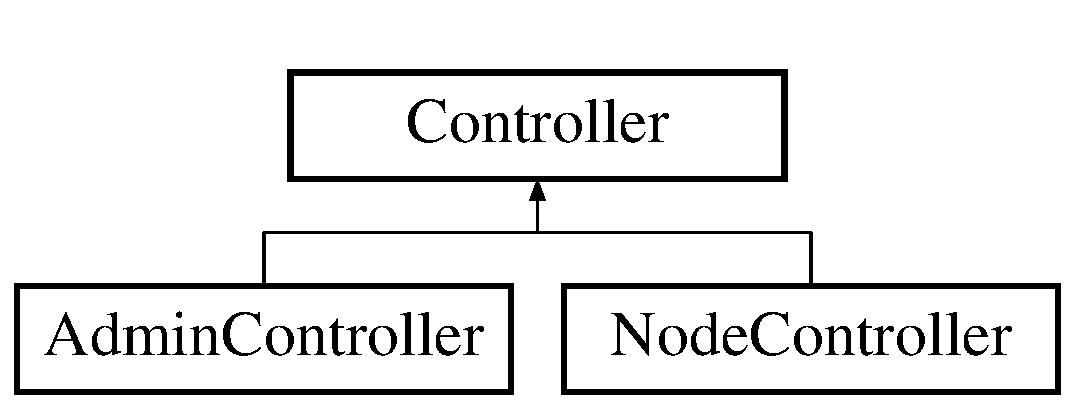
\includegraphics[height=2.000000cm]{class_controller}
\end{center}
\end{figure}
\subsection*{Открытые статические члены}
\begin{DoxyCompactItemize}
\item 
static \hyperlink{class_controller_a4c9227317bc5a987371b5eb4407f75e1}{redirect} (\$url)
\end{DoxyCompactItemize}
\subsection*{Защищенные члены}
\begin{DoxyCompactItemize}
\item 
\hyperlink{class_controller_a87cbafbc85f49bc8864557e1ffe0c143}{render} (array \$args=array(), \$tpl=null)
\begin{DoxyCompactList}\small\item\em Рендеринг обычных страниц \end{DoxyCompactList}\item 
\hyperlink{class_controller_a97e0e46d82368469d174861ca29f2001}{render\-\_\-admin} (array \$args=array(), \$tpl=null)
\end{DoxyCompactItemize}


\subsection{Подробное описание}
Class \hyperlink{class_controller}{Controller}. 

Отвечает за рендеринг, редиректы 

См. определение в файле Controller.\-php строка 9



\subsection{Методы}
\hypertarget{class_controller_a4c9227317bc5a987371b5eb4407f75e1}{\index{Controller@{Controller}!redirect@{redirect}}
\index{redirect@{redirect}!Controller@{Controller}}
\subsubsection[{redirect}]{\setlength{\rightskip}{0pt plus 5cm}static redirect (
\begin{DoxyParamCaption}
\item[{}]{\$url}
\end{DoxyParamCaption}
)\hspace{0.3cm}{\ttfamily [static]}}}\label{class_controller_a4c9227317bc5a987371b5eb4407f75e1}


См. определение в файле Controller.\-php строка 97

\hypertarget{class_controller_a87cbafbc85f49bc8864557e1ffe0c143}{\index{Controller@{Controller}!render@{render}}
\index{render@{render}!Controller@{Controller}}
\subsubsection[{render}]{\setlength{\rightskip}{0pt plus 5cm}render (
\begin{DoxyParamCaption}
\item[{array}]{\$args = {\ttfamily array()}, }
\item[{}]{\$tpl = {\ttfamily null}}
\end{DoxyParamCaption}
)\hspace{0.3cm}{\ttfamily [protected]}}}\label{class_controller_a87cbafbc85f49bc8864557e1ffe0c143}


Рендеринг обычных страниц 


\begin{DoxyParams}{Аргументы}
{\em \$arg} & Массив переменных передаваемые в шаблон для отображения \\
\hline
{\em \$tpl} & имя файла шаблона по умолчанию = null если оно отличается от имени дейстия (Action)\\
\hline
\end{DoxyParams}
Переменные из массива \$args используются в файлах шаблонов для вывода необходимого контента.\-В буфер обмена записывается сначала результат рендеринга необходимого шаблона, результат передается переменной \$content. После этого из буфера обмена выгружатеся вся страница в виде основного шаблона \hyperlink{layout_8phtml}{layout.\-phtml} или \hyperlink{layout__billing_8phtml}{layout\-\_\-billing.\-phtml} в котором встроенна переменная \$content, содержащая основной контент. Используются различные лайауты \hyperlink{layout_8phtml}{layout.\-phtml} или \hyperlink{layout__billing_8phtml}{layout\-\_\-billing.\-phtml} в зависимости от запроса страници -\/ если запрос произошел из биллинга (еслиь get параметр 'bl') -\/layout\-\_\-billing.\-phtml, если запрос из самого приложения обычный лайаут.

\begin{DoxyReturn}{Возвращает}
ob\-\_\-get\-\_\-clean() Отрендеренную страницу из буфера обмена 
\end{DoxyReturn}


См. определение в файле Controller.\-php строка 60

\hypertarget{class_controller_a97e0e46d82368469d174861ca29f2001}{\index{Controller@{Controller}!render\-\_\-admin@{render\-\_\-admin}}
\index{render\-\_\-admin@{render\-\_\-admin}!Controller@{Controller}}
\subsubsection[{render\-\_\-admin}]{\setlength{\rightskip}{0pt plus 5cm}render\-\_\-admin (
\begin{DoxyParamCaption}
\item[{array}]{\$args = {\ttfamily array()}, }
\item[{}]{\$tpl = {\ttfamily null}}
\end{DoxyParamCaption}
)\hspace{0.3cm}{\ttfamily [protected]}}}\label{class_controller_a97e0e46d82368469d174861ca29f2001}


См. определение в файле Controller.\-php строка 80



Объявления и описания членов класса находятся в файле\-:\begin{DoxyCompactItemize}
\item 
/home/artem/public\-\_\-html/test01/\-Library/\hyperlink{_controller_8php}{Controller.\-php}\end{DoxyCompactItemize}

\hypertarget{class_debugger}{\section{Debugger Class Reference}
\label{class_debugger}\index{Debugger@{Debugger}}
}
\subsection*{Static Public Member Functions}
\begin{DoxyCompactItemize}
\item 
\hypertarget{class_debugger_aabc92ba8fe7187ce953d8edbb3175e78}{static {\bfseries Print\-R} (\$item)}\label{class_debugger_aabc92ba8fe7187ce953d8edbb3175e78}

\item 
\hypertarget{class_debugger_a54d5010505863da589f9355a898c4116}{static {\bfseries Var\-Damp} (\$item)}\label{class_debugger_a54d5010505863da589f9355a898c4116}

\end{DoxyCompactItemize}


The documentation for this class was generated from the following file\-:\begin{DoxyCompactItemize}
\item 
Library/Debugger.\-php\end{DoxyCompactItemize}

\hypertarget{classerror_model}{\section{Класс error\-Model}
\label{classerror_model}\index{error\-Model@{error\-Model}}
}
\subsection*{Открытые члены}
\begin{DoxyCompactItemize}
\item 
\hyperlink{classerror_model_a4ed8d21ed582ab26d9d813e9f44251d7}{\-\_\-\-\_\-construct} (\$account\-\_\-id=null, \$switch\-\_\-id=null, \$port\-\_\-id=null, \$switch\-\_\-port\-\_\-id=null)
\item 
\hyperlink{classerror_model_a268a368bcd4dfaa39b9c393dd1c0b858}{write\-Error} (\$error)
\item 
\hyperlink{classerror_model_a5485c7a0cb6321d59632e75c3d945d09}{get\-Error\-Data} (\$date)
\item 
\hyperlink{classerror_model_a2797be2d07b2b4efc973c5584c28d023}{clean\-User\-Error} ()
\end{DoxyCompactItemize}
\subsection*{Поля данных}
\begin{DoxyCompactItemize}
\item 
\hyperlink{classerror_model_af0fcd925f00973e32f7214859dfb3c6b}{\$user\-\_\-id} = null
\item 
\hyperlink{classerror_model_a21ec74990029279615d417ec27831ccf}{\$switch\-\_\-id} = null
\item 
\hyperlink{classerror_model_ad8662b1c3f632fb3bf4b108a062b7474}{\$port\-\_\-id} = null
\item 
\hyperlink{classerror_model_a481c918f8d853749e00b5942cabf599a}{\$date}
\item 
\hyperlink{classerror_model_a78db1a0602e3b6ac1d9a1b5ec103c160}{\$time}
\end{DoxyCompactItemize}


\subsection{Подробное описание}


См. определение в файле error\-Model.\-php строка 4



\subsection{Конструктор(ы)}
\hypertarget{classerror_model_a4ed8d21ed582ab26d9d813e9f44251d7}{\index{error\-Model@{error\-Model}!\-\_\-\-\_\-construct@{\-\_\-\-\_\-construct}}
\index{\-\_\-\-\_\-construct@{\-\_\-\-\_\-construct}!errorModel@{error\-Model}}
\subsubsection[{\-\_\-\-\_\-construct}]{\setlength{\rightskip}{0pt plus 5cm}\-\_\-\-\_\-construct (
\begin{DoxyParamCaption}
\item[{}]{\$account\-\_\-id = {\ttfamily null}, }
\item[{}]{\$switch\-\_\-id = {\ttfamily null}, }
\item[{}]{\$port\-\_\-id = {\ttfamily null}, }
\item[{}]{\$switch\-\_\-port\-\_\-id = {\ttfamily null}}
\end{DoxyParamCaption}
)}}\label{classerror_model_a4ed8d21ed582ab26d9d813e9f44251d7}


См. определение в файле error\-Model.\-php строка 12



\subsection{Методы}
\hypertarget{classerror_model_a2797be2d07b2b4efc973c5584c28d023}{\index{error\-Model@{error\-Model}!clean\-User\-Error@{clean\-User\-Error}}
\index{clean\-User\-Error@{clean\-User\-Error}!errorModel@{error\-Model}}
\subsubsection[{clean\-User\-Error}]{\setlength{\rightskip}{0pt plus 5cm}clean\-User\-Error (
\begin{DoxyParamCaption}
{}
\end{DoxyParamCaption}
)}}\label{classerror_model_a2797be2d07b2b4efc973c5584c28d023}


См. определение в файле error\-Model.\-php строка 89

\hypertarget{classerror_model_a5485c7a0cb6321d59632e75c3d945d09}{\index{error\-Model@{error\-Model}!get\-Error\-Data@{get\-Error\-Data}}
\index{get\-Error\-Data@{get\-Error\-Data}!errorModel@{error\-Model}}
\subsubsection[{get\-Error\-Data}]{\setlength{\rightskip}{0pt plus 5cm}get\-Error\-Data (
\begin{DoxyParamCaption}
\item[{}]{\$date}
\end{DoxyParamCaption}
)}}\label{classerror_model_a5485c7a0cb6321d59632e75c3d945d09}


См. определение в файле error\-Model.\-php строка 67

\hypertarget{classerror_model_a268a368bcd4dfaa39b9c393dd1c0b858}{\index{error\-Model@{error\-Model}!write\-Error@{write\-Error}}
\index{write\-Error@{write\-Error}!errorModel@{error\-Model}}
\subsubsection[{write\-Error}]{\setlength{\rightskip}{0pt plus 5cm}write\-Error (
\begin{DoxyParamCaption}
\item[{}]{\$error}
\end{DoxyParamCaption}
)}}\label{classerror_model_a268a368bcd4dfaa39b9c393dd1c0b858}


См. определение в файле error\-Model.\-php строка 40



\subsection{Поля}
\hypertarget{classerror_model_a481c918f8d853749e00b5942cabf599a}{\index{error\-Model@{error\-Model}!\$date@{\$date}}
\index{\$date@{\$date}!errorModel@{error\-Model}}
\subsubsection[{\$date}]{\setlength{\rightskip}{0pt plus 5cm}\$date}}\label{classerror_model_a481c918f8d853749e00b5942cabf599a}


См. определение в файле error\-Model.\-php строка 9

\hypertarget{classerror_model_ad8662b1c3f632fb3bf4b108a062b7474}{\index{error\-Model@{error\-Model}!\$port\-\_\-id@{\$port\-\_\-id}}
\index{\$port\-\_\-id@{\$port\-\_\-id}!errorModel@{error\-Model}}
\subsubsection[{\$port\-\_\-id}]{\setlength{\rightskip}{0pt plus 5cm}\$port\-\_\-id = null}}\label{classerror_model_ad8662b1c3f632fb3bf4b108a062b7474}


См. определение в файле error\-Model.\-php строка 8

\hypertarget{classerror_model_a21ec74990029279615d417ec27831ccf}{\index{error\-Model@{error\-Model}!\$switch\-\_\-id@{\$switch\-\_\-id}}
\index{\$switch\-\_\-id@{\$switch\-\_\-id}!errorModel@{error\-Model}}
\subsubsection[{\$switch\-\_\-id}]{\setlength{\rightskip}{0pt plus 5cm}\$switch\-\_\-id = null}}\label{classerror_model_a21ec74990029279615d417ec27831ccf}


См. определение в файле error\-Model.\-php строка 7

\hypertarget{classerror_model_a78db1a0602e3b6ac1d9a1b5ec103c160}{\index{error\-Model@{error\-Model}!\$time@{\$time}}
\index{\$time@{\$time}!errorModel@{error\-Model}}
\subsubsection[{\$time}]{\setlength{\rightskip}{0pt plus 5cm}\$time}}\label{classerror_model_a78db1a0602e3b6ac1d9a1b5ec103c160}


См. определение в файле error\-Model.\-php строка 10

\hypertarget{classerror_model_af0fcd925f00973e32f7214859dfb3c6b}{\index{error\-Model@{error\-Model}!\$user\-\_\-id@{\$user\-\_\-id}}
\index{\$user\-\_\-id@{\$user\-\_\-id}!errorModel@{error\-Model}}
\subsubsection[{\$user\-\_\-id}]{\setlength{\rightskip}{0pt plus 5cm}\$user\-\_\-id = null}}\label{classerror_model_af0fcd925f00973e32f7214859dfb3c6b}


См. определение в файле error\-Model.\-php строка 6



Объявления и описания членов класса находятся в файле\-:\begin{DoxyCompactItemize}
\item 
/home/artem/public\-\_\-html/test01/\-Model/\hyperlink{error_model_8php}{error\-Model.\-php}\end{DoxyCompactItemize}

\hypertarget{classhelper_model}{\section{Класс helper\-Model}
\label{classhelper_model}\index{helper\-Model@{helper\-Model}}
}
\subsection*{Открытые члены}
\begin{DoxyCompactItemize}
\item 
\hyperlink{classhelper_model_a64e87d3c9076ef6df046354edbc5b237}{insert\-Mac} (\$id, \$mac, \$switch\-\_\-ip, \$port, \$switch\-\_\-model, \$firmware, \$manufacturer)
\end{DoxyCompactItemize}


\subsection{Подробное описание}


См. определение в файле helper\-Model.\-php строка 4



\subsection{Методы}
\hypertarget{classhelper_model_a64e87d3c9076ef6df046354edbc5b237}{\index{helper\-Model@{helper\-Model}!insert\-Mac@{insert\-Mac}}
\index{insert\-Mac@{insert\-Mac}!helperModel@{helper\-Model}}
\subsubsection[{insert\-Mac}]{\setlength{\rightskip}{0pt plus 5cm}insert\-Mac (
\begin{DoxyParamCaption}
\item[{}]{\$id, }
\item[{}]{\$mac, }
\item[{}]{\$switch\-\_\-ip, }
\item[{}]{\$port, }
\item[{}]{\$switch\-\_\-model, }
\item[{}]{\$firmware, }
\item[{}]{\$manufacturer}
\end{DoxyParamCaption}
)}}\label{classhelper_model_a64e87d3c9076ef6df046354edbc5b237}


См. определение в файле helper\-Model.\-php строка 6



Объявления и описания членов класса находятся в файле\-:\begin{DoxyCompactItemize}
\item 
/home/artem/public\-\_\-html/test01/\-Model/\hyperlink{helper_model_8php}{helper\-Model.\-php}\end{DoxyCompactItemize}

\hypertarget{classhistory_model}{\section{history\-Model Class Reference}
\label{classhistory_model}\index{history\-Model@{history\-Model}}
}
\subsection*{Public Member Functions}
\begin{DoxyCompactItemize}
\item 
\hypertarget{classhistory_model_a35350490d1e0f0597011c9b01f8a5810}{{\bfseries insert\-Data} (\$account\-\_\-id, array \$data\-\_\-switch, array \$data\-\_\-db)}\label{classhistory_model_a35350490d1e0f0597011c9b01f8a5810}

\item 
\hypertarget{classhistory_model_a4025876f36ec47a3b8fc7c98d6d3f60c}{{\bfseries select\-Data} (\$account\-\_\-id)}\label{classhistory_model_a4025876f36ec47a3b8fc7c98d6d3f60c}

\item 
\hypertarget{classhistory_model_a2761da68d4037399261d683ab4f9b2b7}{{\bfseries clean\-History} ()}\label{classhistory_model_a2761da68d4037399261d683ab4f9b2b7}

\end{DoxyCompactItemize}


The documentation for this class was generated from the following file\-:\begin{DoxyCompactItemize}
\item 
Model/history\-Model.\-php\end{DoxyCompactItemize}

\hypertarget{class_index_model}{\section{Класс Index\-Model}
\label{class_index_model}\index{Index\-Model@{Index\-Model}}
}
\subsection*{Открытые члены}
\begin{DoxyCompactItemize}
\item 
\hyperlink{class_index_model_a5cdd544cd52782642a0f42334acdb531}{snmp\-Data} (\$account\-\_\-id, \$key, \$variable=null, \$switch\-\_\-id=null, \$port\-\_\-id=null)
\item 
\hyperlink{class_index_model_a395d66b37a253bab5365dbee626e7dbd}{get\-All\-Mac} (\$account\-\_\-id, \$pattern\-\_\-id, array \$port\-\_\-coefficient, \$switch\-\_\-id=null, \$port\-\_\-id=null)
\item 
\hyperlink{class_index_model_a92cfbe87f525727795f818072f74bb16}{cable\-Test} (\$account\-\_\-id, \$pattern\-\_\-id, \$port, \$switch\-\_\-manufacturer, \$style\-\_\-class=null, \$switch\-\_\-id=null)
\item 
\hyperlink{class_index_model_a1fce7d860847195080702dd2174e198c}{get\-Community} ()
\item 
\hyperlink{class_index_model_a99d3df1e9eea9f8bbe8be04067299e1c}{index\-Page} (\$id)
\item 
\hyperlink{class_index_model_afcec9844f30bbb9cdaf48fac789e1d7b}{snmp\-By\-Key} (\$account\-\_\-id, \$key, \$switch\-\_\-id=null, \$port\-\_\-id=null)
\item 
\hyperlink{class_index_model_ad90f0c96df11bdd429c62fa31cf226e3}{user\-Id\-By\-Port} (\$port, \$switch\-\_\-id)
\item 
\hyperlink{class_index_model_ae8029f54b6dbca39a2c9c8c80e5d24d1}{get\-Port\-Coefficient} (\$account\-\_\-id, \$port\-\_\-number, \$switch\-\_\-id)
\item 
\hyperlink{class_index_model_ad0fb7f4d93efd7678f7136d32990ee6f}{get\-User\-By\-Mac} (\$mac)
\end{DoxyCompactItemize}
\subsection*{Открытые статические члены}
\begin{DoxyCompactItemize}
\item 
static \hyperlink{class_index_model_ab17dd49d3409d5f198dffea22b33bce2}{get\-Port\-Coeff} ()
\end{DoxyCompactItemize}


\subsection{Подробное описание}


См. определение в файле Index\-Model.\-php строка 4



\subsection{Методы}
\hypertarget{class_index_model_a92cfbe87f525727795f818072f74bb16}{\index{Index\-Model@{Index\-Model}!cable\-Test@{cable\-Test}}
\index{cable\-Test@{cable\-Test}!IndexModel@{Index\-Model}}
\subsubsection[{cable\-Test}]{\setlength{\rightskip}{0pt plus 5cm}cable\-Test (
\begin{DoxyParamCaption}
\item[{}]{\$account\-\_\-id, }
\item[{}]{\$pattern\-\_\-id, }
\item[{}]{\$port, }
\item[{}]{\$switch\-\_\-manufacturer, }
\item[{}]{\$style\-\_\-class = {\ttfamily null}, }
\item[{}]{\$switch\-\_\-id = {\ttfamily null}}
\end{DoxyParamCaption}
)}}\label{class_index_model_a92cfbe87f525727795f818072f74bb16}


См. определение в файле Index\-Model.\-php строка 291

\hypertarget{class_index_model_a395d66b37a253bab5365dbee626e7dbd}{\index{Index\-Model@{Index\-Model}!get\-All\-Mac@{get\-All\-Mac}}
\index{get\-All\-Mac@{get\-All\-Mac}!IndexModel@{Index\-Model}}
\subsubsection[{get\-All\-Mac}]{\setlength{\rightskip}{0pt plus 5cm}get\-All\-Mac (
\begin{DoxyParamCaption}
\item[{}]{\$account\-\_\-id, }
\item[{}]{\$pattern\-\_\-id, }
\item[{array}]{\$port\-\_\-coefficient, }
\item[{}]{\$switch\-\_\-id = {\ttfamily null}, }
\item[{}]{\$port\-\_\-id = {\ttfamily null}}
\end{DoxyParamCaption}
)}}\label{class_index_model_a395d66b37a253bab5365dbee626e7dbd}


См. определение в файле Index\-Model.\-php строка 271

\hypertarget{class_index_model_a1fce7d860847195080702dd2174e198c}{\index{Index\-Model@{Index\-Model}!get\-Community@{get\-Community}}
\index{get\-Community@{get\-Community}!IndexModel@{Index\-Model}}
\subsubsection[{get\-Community}]{\setlength{\rightskip}{0pt plus 5cm}get\-Community (
\begin{DoxyParamCaption}
{}
\end{DoxyParamCaption}
)}}\label{class_index_model_a1fce7d860847195080702dd2174e198c}


См. определение в файле Index\-Model.\-php строка 319

\hypertarget{class_index_model_ab17dd49d3409d5f198dffea22b33bce2}{\index{Index\-Model@{Index\-Model}!get\-Port\-Coeff@{get\-Port\-Coeff}}
\index{get\-Port\-Coeff@{get\-Port\-Coeff}!IndexModel@{Index\-Model}}
\subsubsection[{get\-Port\-Coeff}]{\setlength{\rightskip}{0pt plus 5cm}static get\-Port\-Coeff (
\begin{DoxyParamCaption}
{}
\end{DoxyParamCaption}
)\hspace{0.3cm}{\ttfamily [static]}}}\label{class_index_model_ab17dd49d3409d5f198dffea22b33bce2}
\begin{DoxyReturn}{Возвращает}
array 
\end{DoxyReturn}


См. определение в файле Index\-Model.\-php строка 438

\hypertarget{class_index_model_ae8029f54b6dbca39a2c9c8c80e5d24d1}{\index{Index\-Model@{Index\-Model}!get\-Port\-Coefficient@{get\-Port\-Coefficient}}
\index{get\-Port\-Coefficient@{get\-Port\-Coefficient}!IndexModel@{Index\-Model}}
\subsubsection[{get\-Port\-Coefficient}]{\setlength{\rightskip}{0pt plus 5cm}get\-Port\-Coefficient (
\begin{DoxyParamCaption}
\item[{}]{\$account\-\_\-id, }
\item[{}]{\$port\-\_\-number, }
\item[{}]{\$switch\-\_\-id}
\end{DoxyParamCaption}
)}}\label{class_index_model_ae8029f54b6dbca39a2c9c8c80e5d24d1}


См. определение в файле Index\-Model.\-php строка 381

\hypertarget{class_index_model_ad0fb7f4d93efd7678f7136d32990ee6f}{\index{Index\-Model@{Index\-Model}!get\-User\-By\-Mac@{get\-User\-By\-Mac}}
\index{get\-User\-By\-Mac@{get\-User\-By\-Mac}!IndexModel@{Index\-Model}}
\subsubsection[{get\-User\-By\-Mac}]{\setlength{\rightskip}{0pt plus 5cm}get\-User\-By\-Mac (
\begin{DoxyParamCaption}
\item[{}]{\$mac}
\end{DoxyParamCaption}
)}}\label{class_index_model_ad0fb7f4d93efd7678f7136d32990ee6f}


См. определение в файле Index\-Model.\-php строка 422

\hypertarget{class_index_model_a99d3df1e9eea9f8bbe8be04067299e1c}{\index{Index\-Model@{Index\-Model}!index\-Page@{index\-Page}}
\index{index\-Page@{index\-Page}!IndexModel@{Index\-Model}}
\subsubsection[{index\-Page}]{\setlength{\rightskip}{0pt plus 5cm}index\-Page (
\begin{DoxyParamCaption}
\item[{}]{\$id}
\end{DoxyParamCaption}
)}}\label{class_index_model_a99d3df1e9eea9f8bbe8be04067299e1c}


См. определение в файле Index\-Model.\-php строка 343

\hypertarget{class_index_model_afcec9844f30bbb9cdaf48fac789e1d7b}{\index{Index\-Model@{Index\-Model}!snmp\-By\-Key@{snmp\-By\-Key}}
\index{snmp\-By\-Key@{snmp\-By\-Key}!IndexModel@{Index\-Model}}
\subsubsection[{snmp\-By\-Key}]{\setlength{\rightskip}{0pt plus 5cm}snmp\-By\-Key (
\begin{DoxyParamCaption}
\item[{}]{\$account\-\_\-id, }
\item[{}]{\$key, }
\item[{}]{\$switch\-\_\-id = {\ttfamily null}, }
\item[{}]{\$port\-\_\-id = {\ttfamily null}}
\end{DoxyParamCaption}
)}}\label{class_index_model_afcec9844f30bbb9cdaf48fac789e1d7b}


См. определение в файле Index\-Model.\-php строка 355

\hypertarget{class_index_model_a5cdd544cd52782642a0f42334acdb531}{\index{Index\-Model@{Index\-Model}!snmp\-Data@{snmp\-Data}}
\index{snmp\-Data@{snmp\-Data}!IndexModel@{Index\-Model}}
\subsubsection[{snmp\-Data}]{\setlength{\rightskip}{0pt plus 5cm}snmp\-Data (
\begin{DoxyParamCaption}
\item[{}]{\$account\-\_\-id, }
\item[{}]{\$key, }
\item[{}]{\$variable = {\ttfamily null}, }
\item[{}]{\$switch\-\_\-id = {\ttfamily null}, }
\item[{}]{\$port\-\_\-id = {\ttfamily null}}
\end{DoxyParamCaption}
)}}\label{class_index_model_a5cdd544cd52782642a0f42334acdb531}


См. определение в файле Index\-Model.\-php строка 82

\hypertarget{class_index_model_ad90f0c96df11bdd429c62fa31cf226e3}{\index{Index\-Model@{Index\-Model}!user\-Id\-By\-Port@{user\-Id\-By\-Port}}
\index{user\-Id\-By\-Port@{user\-Id\-By\-Port}!IndexModel@{Index\-Model}}
\subsubsection[{user\-Id\-By\-Port}]{\setlength{\rightskip}{0pt plus 5cm}user\-Id\-By\-Port (
\begin{DoxyParamCaption}
\item[{}]{\$port, }
\item[{}]{\$switch\-\_\-id}
\end{DoxyParamCaption}
)}}\label{class_index_model_ad90f0c96df11bdd429c62fa31cf226e3}


См. определение в файле Index\-Model.\-php строка 366



Объявления и описания членов класса находятся в файле\-:\begin{DoxyCompactItemize}
\item 
/home/artem/public\-\_\-html/test01/\-Model/\hyperlink{_index_model_8php}{Index\-Model.\-php}\end{DoxyCompactItemize}

\hypertarget{class_node_controller}{\section{Класс Node\-Controller}
\label{class_node_controller}\index{Node\-Controller@{Node\-Controller}}
}


Class \hyperlink{class_node_controller}{Node\-Controller}.  


Граф наследования\-:Node\-Controller\-:\begin{figure}[H]
\begin{center}
\leavevmode
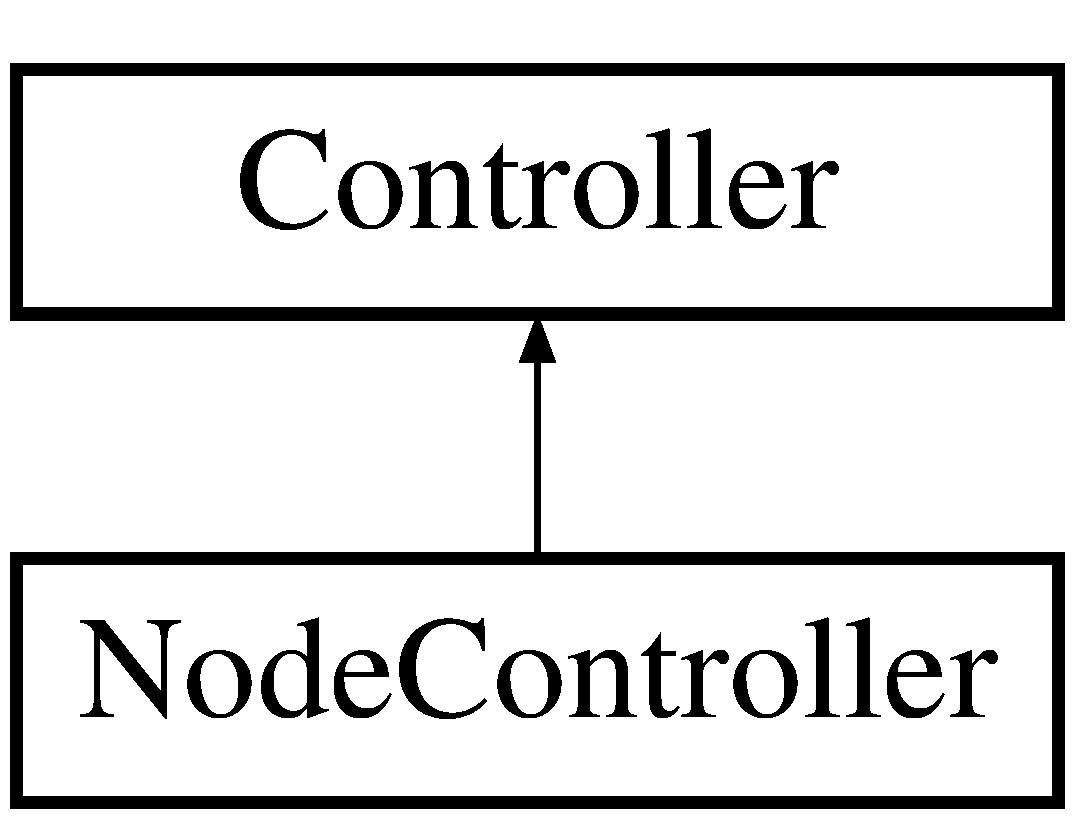
\includegraphics[height=2.000000cm]{class_node_controller}
\end{center}
\end{figure}
\subsection*{Открытые члены}
\begin{DoxyCompactItemize}
\item 
\hyperlink{class_node_controller_a04f2101fe1cdc785b61219c2df753024}{index\-Action} ()
\begin{DoxyCompactList}\small\item\em Action отвечате за загрузку обычных страниц(включая стандартных страниц ошибок) \end{DoxyCompactList}\end{DoxyCompactItemize}
\subsection*{Открытые статические члены}
\begin{DoxyCompactItemize}
\item 
static \hyperlink{class_node_controller_a2d13f67877bc056bc6798b3d0931c4a2}{write\-Error\-Data} (Exception \$e)
\begin{DoxyCompactList}\small\item\em Обработка информации выброшенных исключений \end{DoxyCompactList}\end{DoxyCompactItemize}
\subsection*{Дополнительные унаследованные члены}


\subsection{Подробное описание}
Class \hyperlink{class_node_controller}{Node\-Controller}. 

Class \hyperlink{class_node_controller}{Node\-Controller} отвечает за загрузку страниц приложения. Включает метод для загрузки стандартных страниц и страниц ошибок. Также write\-Error\-Data записывает на страницах ошибок информацию полученную из выброшенных исключений. 

См. определение в файле Node\-Controller.\-php строка 9



\subsection{Методы}
\hypertarget{class_node_controller_a04f2101fe1cdc785b61219c2df753024}{\index{Node\-Controller@{Node\-Controller}!index\-Action@{index\-Action}}
\index{index\-Action@{index\-Action}!NodeController@{Node\-Controller}}
\subsubsection[{index\-Action}]{\setlength{\rightskip}{0pt plus 5cm}index\-Action (
\begin{DoxyParamCaption}
{}
\end{DoxyParamCaption}
)}}\label{class_node_controller_a04f2101fe1cdc785b61219c2df753024}


Action отвечате за загрузку обычных страниц(включая стандартных страниц ошибок) 

Action отвечате за загрузку обычных страниц(включая стандартных страниц ошибок). Данные о необходимой странице передает объект класса \hyperlink{class_node_model}{Node\-Model}, id нужной страници получает роутер (\hyperlink{class_router}{Router}) при парсинге url. \$args массив содержит контент страници полученный \hyperlink{class_node_model}{Node\-Model} моделью из базы данных а также данные о выброшенном исключении. Передается аргументом в возвращаемую функцию рендеринга \$this-\/$>$render(\$args) \begin{DoxyReturn}{Возвращает}
\$this-\/$>$render(\$args) Функция рендеринга страници с параметром \$args 
\end{DoxyReturn}


См. определение в файле Node\-Controller.\-php строка 39

\hypertarget{class_node_controller_a2d13f67877bc056bc6798b3d0931c4a2}{\index{Node\-Controller@{Node\-Controller}!write\-Error\-Data@{write\-Error\-Data}}
\index{write\-Error\-Data@{write\-Error\-Data}!NodeController@{Node\-Controller}}
\subsubsection[{write\-Error\-Data}]{\setlength{\rightskip}{0pt plus 5cm}static write\-Error\-Data (
\begin{DoxyParamCaption}
\item[{Exception}]{\$e}
\end{DoxyParamCaption}
)\hspace{0.3cm}{\ttfamily [static]}}}\label{class_node_controller_a2d13f67877bc056bc6798b3d0931c4a2}


Обработка информации выброшенных исключений 


\begin{DoxyParams}[1]{Аргументы}
Exception & {\em \$e} & объект выброшенного исключения\\
\hline
\end{DoxyParams}
Записывает в свойства класса код ошибки и сообщение полученное из объекта \$e выброшенного исключения 

См. определение в файле Node\-Controller.\-php строка 23



Объявления и описания членов класса находятся в файле\-:\begin{DoxyCompactItemize}
\item 
/home/artem/public\-\_\-html/test01/\-Controller/\hyperlink{_node_controller_8php}{Node\-Controller.\-php}\end{DoxyCompactItemize}

\hypertarget{class_node_model}{\section{Node\-Model Class Reference}
\label{class_node_model}\index{Node\-Model@{Node\-Model}}
}
\subsection*{Public Member Functions}
\begin{DoxyCompactItemize}
\item 
\hypertarget{class_node_model_a99d3df1e9eea9f8bbe8be04067299e1c}{{\bfseries index\-Page} (\$id)}\label{class_node_model_a99d3df1e9eea9f8bbe8be04067299e1c}

\end{DoxyCompactItemize}


The documentation for this class was generated from the following file\-:\begin{DoxyCompactItemize}
\item 
Model/Node\-Model.\-php\end{DoxyCompactItemize}

\hypertarget{classpattern_model}{\section{pattern\-Model Class Reference}
\label{classpattern_model}\index{pattern\-Model@{pattern\-Model}}
}
\subsection*{Public Member Functions}
\begin{DoxyCompactItemize}
\item 
\hypertarget{classpattern_model_ae207f7fe29d94a4271fb32a156b4ce64}{{\bfseries \-\_\-\-\_\-construct} (\$account\-\_\-id)}\label{classpattern_model_ae207f7fe29d94a4271fb32a156b4ce64}

\item 
\hypertarget{classpattern_model_a4f92dd070690a6c938d15a9363065351}{{\bfseries switch\-Data} ()}\label{classpattern_model_a4f92dd070690a6c938d15a9363065351}

\item 
\hypertarget{classpattern_model_a12a4b27a766b5c4573d24e255d1ef5a4}{{\bfseries get\-Pattern\-User\-Data} ()}\label{classpattern_model_a12a4b27a766b5c4573d24e255d1ef5a4}

\item 
\hypertarget{classpattern_model_a5c106765af75e3a68d2191cdc2d784f3}{{\bfseries Pattern\-Data} (\$port\-\_\-number, \$pattern\-\_\-id)}\label{classpattern_model_a5c106765af75e3a68d2191cdc2d784f3}

\item 
\hypertarget{classpattern_model_a31f25239e28e31eb5baa5ab4564675b8}{{\bfseries mac\-Data} (\$pattern\-\_\-id)}\label{classpattern_model_a31f25239e28e31eb5baa5ab4564675b8}

\item 
\hypertarget{classpattern_model_a0f19e4f669687aaa80334bd503890fa7}{{\bfseries get\-Port\-Coefficient} (\$pattern\-\_\-id)}\label{classpattern_model_a0f19e4f669687aaa80334bd503890fa7}

\end{DoxyCompactItemize}
\subsection*{Data Fields}
\begin{DoxyCompactItemize}
\item 
\hypertarget{classpattern_model_a7c3eb7a98818df12bc88e63ac7ea9c63}{{\bfseries \$account\-\_\-id}}\label{classpattern_model_a7c3eb7a98818df12bc88e63ac7ea9c63}

\end{DoxyCompactItemize}


The documentation for this class was generated from the following file\-:\begin{DoxyCompactItemize}
\item 
Model/pattern\-Model.\-php\end{DoxyCompactItemize}

\hypertarget{class_request}{\section{Класс Request}
\label{class_request}\index{Request@{Request}}
}
\subsection*{Открытые члены}
\begin{DoxyCompactItemize}
\item 
\hyperlink{class_request_a095c5d389db211932136b53f25f39685}{\-\_\-\-\_\-construct} ()
\item 
\hyperlink{class_request_a24a9bf83a1002d46ece83a93d14bd921}{get} (\$key)
\item 
\hyperlink{class_request_a00ba439ffbc7a78df5f313ad780503d2}{post} (\$key)
\item 
\hyperlink{class_request_a53b35eef049be6f323fd8066b37d6be6}{server} (\$key)
\item 
\hyperlink{class_request_a938a7fa5c2633579704b0f4a3ded2d01}{files} (\$key)
\item 
\hyperlink{class_request_a2d62038e063e771c2fd920155f344d58}{is\-Post} ()
\end{DoxyCompactItemize}


\subsection{Подробное описание}


См. определение в файле Request.\-php строка 4



\subsection{Конструктор(ы)}
\hypertarget{class_request_a095c5d389db211932136b53f25f39685}{\index{Request@{Request}!\-\_\-\-\_\-construct@{\-\_\-\-\_\-construct}}
\index{\-\_\-\-\_\-construct@{\-\_\-\-\_\-construct}!Request@{Request}}
\subsubsection[{\-\_\-\-\_\-construct}]{\setlength{\rightskip}{0pt plus 5cm}\-\_\-\-\_\-construct (
\begin{DoxyParamCaption}
{}
\end{DoxyParamCaption}
)}}\label{class_request_a095c5d389db211932136b53f25f39685}


См. определение в файле Request.\-php строка 19



\subsection{Методы}
\hypertarget{class_request_a938a7fa5c2633579704b0f4a3ded2d01}{\index{Request@{Request}!files@{files}}
\index{files@{files}!Request@{Request}}
\subsubsection[{files}]{\setlength{\rightskip}{0pt plus 5cm}files (
\begin{DoxyParamCaption}
\item[{}]{\$key}
\end{DoxyParamCaption}
)}}\label{class_request_a938a7fa5c2633579704b0f4a3ded2d01}


См. определение в файле Request.\-php строка 44

\hypertarget{class_request_a24a9bf83a1002d46ece83a93d14bd921}{\index{Request@{Request}!get@{get}}
\index{get@{get}!Request@{Request}}
\subsubsection[{get}]{\setlength{\rightskip}{0pt plus 5cm}get (
\begin{DoxyParamCaption}
\item[{}]{\$key}
\end{DoxyParamCaption}
)}}\label{class_request_a24a9bf83a1002d46ece83a93d14bd921}


См. определение в файле Request.\-php строка 28

\hypertarget{class_request_a2d62038e063e771c2fd920155f344d58}{\index{Request@{Request}!is\-Post@{is\-Post}}
\index{is\-Post@{is\-Post}!Request@{Request}}
\subsubsection[{is\-Post}]{\setlength{\rightskip}{0pt plus 5cm}is\-Post (
\begin{DoxyParamCaption}
{}
\end{DoxyParamCaption}
)}}\label{class_request_a2d62038e063e771c2fd920155f344d58}


См. определение в файле Request.\-php строка 52

\hypertarget{class_request_a00ba439ffbc7a78df5f313ad780503d2}{\index{Request@{Request}!post@{post}}
\index{post@{post}!Request@{Request}}
\subsubsection[{post}]{\setlength{\rightskip}{0pt plus 5cm}post (
\begin{DoxyParamCaption}
\item[{}]{\$key}
\end{DoxyParamCaption}
)}}\label{class_request_a00ba439ffbc7a78df5f313ad780503d2}


См. определение в файле Request.\-php строка 33

\hypertarget{class_request_a53b35eef049be6f323fd8066b37d6be6}{\index{Request@{Request}!server@{server}}
\index{server@{server}!Request@{Request}}
\subsubsection[{server}]{\setlength{\rightskip}{0pt plus 5cm}server (
\begin{DoxyParamCaption}
\item[{}]{\$key}
\end{DoxyParamCaption}
)}}\label{class_request_a53b35eef049be6f323fd8066b37d6be6}


См. определение в файле Request.\-php строка 39



Объявления и описания членов класса находятся в файле\-:\begin{DoxyCompactItemize}
\item 
/home/artem/public\-\_\-html/test01/\-Library/\hyperlink{_request_8php}{Request.\-php}\end{DoxyCompactItemize}

\hypertarget{class_router}{\section{Router Class Reference}
\label{class_router}\index{Router@{Router}}
}
\subsection*{Static Public Member Functions}
\begin{DoxyCompactItemize}
\item 
static \hyperlink{class_router_ad6b0d5b03226bb27efd8c410c89ef635}{parse} (\$url)
\item 
\hypertarget{class_router_a7e384b5b08035be60df7696428c6cf56}{static {\bfseries get\-\_\-content\-\_\-by\-\_\-url} (\$url)}\label{class_router_a7e384b5b08035be60df7696428c6cf56}

\item 
static \hyperlink{class_router_a45e9b6bbc2e0abd383bf9a788db25dab}{get\-Url} (\$route\-Name, array \$params=array())
\item 
static \hyperlink{class_router_a0c5216068060ca9253dbad31e5895a2b}{get\-Controller} ()
\item 
static \hyperlink{class_router_af8b331d3ac442a1071aa9f7db3b60637}{get\-Action} ()
\item 
\hypertarget{class_router_a0613d1215434e1b563a42dfcd05aad60}{static {\bfseries get\-Account\-Id} ()}\label{class_router_a0613d1215434e1b563a42dfcd05aad60}

\item 
\hypertarget{class_router_acfaa3a96d0cb5a4c0d4d710dcba41e9e}{static {\bfseries get\-Id} ()}\label{class_router_acfaa3a96d0cb5a4c0d4d710dcba41e9e}

\end{DoxyCompactItemize}


\subsection{Member Function Documentation}
\hypertarget{class_router_af8b331d3ac442a1071aa9f7db3b60637}{\index{Router@{Router}!get\-Action@{get\-Action}}
\index{get\-Action@{get\-Action}!Router@{Router}}
\subsubsection[{get\-Action}]{\setlength{\rightskip}{0pt plus 5cm}static get\-Action (
\begin{DoxyParamCaption}
{}
\end{DoxyParamCaption}
)\hspace{0.3cm}{\ttfamily [static]}}}\label{class_router_af8b331d3ac442a1071aa9f7db3b60637}
\begin{DoxyReturn}{Returns}
mixed 
\end{DoxyReturn}
\hypertarget{class_router_a0c5216068060ca9253dbad31e5895a2b}{\index{Router@{Router}!get\-Controller@{get\-Controller}}
\index{get\-Controller@{get\-Controller}!Router@{Router}}
\subsubsection[{get\-Controller}]{\setlength{\rightskip}{0pt plus 5cm}static get\-Controller (
\begin{DoxyParamCaption}
{}
\end{DoxyParamCaption}
)\hspace{0.3cm}{\ttfamily [static]}}}\label{class_router_a0c5216068060ca9253dbad31e5895a2b}
\begin{DoxyReturn}{Returns}
mixed 
\end{DoxyReturn}
\hypertarget{class_router_a45e9b6bbc2e0abd383bf9a788db25dab}{\index{Router@{Router}!get\-Url@{get\-Url}}
\index{get\-Url@{get\-Url}!Router@{Router}}
\subsubsection[{get\-Url}]{\setlength{\rightskip}{0pt plus 5cm}static get\-Url (
\begin{DoxyParamCaption}
\item[{}]{\$route\-Name, }
\item[{array}]{\$params = {\ttfamily array()}}
\end{DoxyParamCaption}
)\hspace{0.3cm}{\ttfamily [static]}}}\label{class_router_a45e9b6bbc2e0abd383bf9a788db25dab}

\begin{DoxyParams}[1]{Parameters}
 & {\em \$route\-Name} & \\
\hline
array & {\em \$params} & \\
\hline
\end{DoxyParams}
\hypertarget{class_router_ad6b0d5b03226bb27efd8c410c89ef635}{\index{Router@{Router}!parse@{parse}}
\index{parse@{parse}!Router@{Router}}
\subsubsection[{parse}]{\setlength{\rightskip}{0pt plus 5cm}static parse (
\begin{DoxyParamCaption}
\item[{}]{\$url}
\end{DoxyParamCaption}
)\hspace{0.3cm}{\ttfamily [static]}}}\label{class_router_ad6b0d5b03226bb27efd8c410c89ef635}

\begin{DoxyParams}{Parameters}
{\em \$url} & \\
\hline
\end{DoxyParams}

\begin{DoxyExceptions}{Exceptions}
{\em Exception} & \\
\hline
\end{DoxyExceptions}


The documentation for this class was generated from the following file\-:\begin{DoxyCompactItemize}
\item 
Library/Router.\-php\end{DoxyCompactItemize}

\hypertarget{class_session}{\section{Класс Session}
\label{class_session}\index{Session@{Session}}
}
\subsection*{Открытые статические члены}
\begin{DoxyCompactItemize}
\item 
static \hyperlink{class_session_a8f660283f72e0f3c5f00b4f98563a79b}{has} (\$key)
\item 
static \hyperlink{class_session_a4ecf4c33104949ba1a007a73d71dbb15}{set} (\$key, \$val)
\item 
static \hyperlink{class_session_a292b7d28cfcd001085631b11754a3a67}{has\-User} (\$user\-\_\-name)
\item 
static \hyperlink{class_session_a15e2679f2a8f6fa4d60757f4d65413ac}{get} (\$key)
\item 
static \hyperlink{class_session_acc60f64095c2df2c0d1e48f9f3ffb9d8}{remove} (\$key)
\item 
static \hyperlink{class_session_a146085d0f3a9d17bdcd7f3d4081d8c0d}{start} ()
\item 
static \hyperlink{class_session_a93d4348dfe017e3b97a7131f03897121}{destroy} ()
\item 
static \hyperlink{class_session_aa7c4da247e52be9a1eb10db617faba68}{set\-Flash} (\$message, \$warning\-\_\-class=null)
\item 
static \hyperlink{class_session_ae4c4b98671bdd1fbfe4ae9defb5405ad}{get\-Flash} (\$account\-\_\-id=null, \$switch\-\_\-id=null, \$port\-\_\-id=null, \$switch\-\_\-port\-\_\-id=null)
\end{DoxyCompactItemize}
\subsection*{Статические открытые данные}
\begin{DoxyCompactItemize}
\item 
static \hyperlink{class_session_a5bacf7bbae287dfd28fbaad90f463720}{\$flash\-\_\-messages} = array()
\end{DoxyCompactItemize}


\subsection{Подробное описание}


См. определение в файле Session.\-php строка 4



\subsection{Методы}
\hypertarget{class_session_a93d4348dfe017e3b97a7131f03897121}{\index{Session@{Session}!destroy@{destroy}}
\index{destroy@{destroy}!Session@{Session}}
\subsubsection[{destroy}]{\setlength{\rightskip}{0pt plus 5cm}static destroy (
\begin{DoxyParamCaption}
{}
\end{DoxyParamCaption}
)\hspace{0.3cm}{\ttfamily [static]}}}\label{class_session_a93d4348dfe017e3b97a7131f03897121}


См. определение в файле Session.\-php строка 48

\hypertarget{class_session_a15e2679f2a8f6fa4d60757f4d65413ac}{\index{Session@{Session}!get@{get}}
\index{get@{get}!Session@{Session}}
\subsubsection[{get}]{\setlength{\rightskip}{0pt plus 5cm}static get (
\begin{DoxyParamCaption}
\item[{}]{\$key}
\end{DoxyParamCaption}
)\hspace{0.3cm}{\ttfamily [static]}}}\label{class_session_a15e2679f2a8f6fa4d60757f4d65413ac}


См. определение в файле Session.\-php строка 28

\hypertarget{class_session_ae4c4b98671bdd1fbfe4ae9defb5405ad}{\index{Session@{Session}!get\-Flash@{get\-Flash}}
\index{get\-Flash@{get\-Flash}!Session@{Session}}
\subsubsection[{get\-Flash}]{\setlength{\rightskip}{0pt plus 5cm}static get\-Flash (
\begin{DoxyParamCaption}
\item[{}]{\$account\-\_\-id = {\ttfamily null}, }
\item[{}]{\$switch\-\_\-id = {\ttfamily null}, }
\item[{}]{\$port\-\_\-id = {\ttfamily null}, }
\item[{}]{\$switch\-\_\-port\-\_\-id = {\ttfamily null}}
\end{DoxyParamCaption}
)\hspace{0.3cm}{\ttfamily [static]}}}\label{class_session_ae4c4b98671bdd1fbfe4ae9defb5405ad}


См. определение в файле Session.\-php строка 74

\hypertarget{class_session_a8f660283f72e0f3c5f00b4f98563a79b}{\index{Session@{Session}!has@{has}}
\index{has@{has}!Session@{Session}}
\subsubsection[{has}]{\setlength{\rightskip}{0pt plus 5cm}static has (
\begin{DoxyParamCaption}
\item[{}]{\$key}
\end{DoxyParamCaption}
)\hspace{0.3cm}{\ttfamily [static]}}}\label{class_session_a8f660283f72e0f3c5f00b4f98563a79b}


См. определение в файле Session.\-php строка 8

\hypertarget{class_session_a292b7d28cfcd001085631b11754a3a67}{\index{Session@{Session}!has\-User@{has\-User}}
\index{has\-User@{has\-User}!Session@{Session}}
\subsubsection[{has\-User}]{\setlength{\rightskip}{0pt plus 5cm}static has\-User (
\begin{DoxyParamCaption}
\item[{}]{\$user\-\_\-name}
\end{DoxyParamCaption}
)\hspace{0.3cm}{\ttfamily [static]}}}\label{class_session_a292b7d28cfcd001085631b11754a3a67}


См. определение в файле Session.\-php строка 20

\hypertarget{class_session_acc60f64095c2df2c0d1e48f9f3ffb9d8}{\index{Session@{Session}!remove@{remove}}
\index{remove@{remove}!Session@{Session}}
\subsubsection[{remove}]{\setlength{\rightskip}{0pt plus 5cm}static remove (
\begin{DoxyParamCaption}
\item[{}]{\$key}
\end{DoxyParamCaption}
)\hspace{0.3cm}{\ttfamily [static]}}}\label{class_session_acc60f64095c2df2c0d1e48f9f3ffb9d8}


См. определение в файле Session.\-php строка 36

\hypertarget{class_session_a4ecf4c33104949ba1a007a73d71dbb15}{\index{Session@{Session}!set@{set}}
\index{set@{set}!Session@{Session}}
\subsubsection[{set}]{\setlength{\rightskip}{0pt plus 5cm}static set (
\begin{DoxyParamCaption}
\item[{}]{\$key, }
\item[{}]{\$val}
\end{DoxyParamCaption}
)\hspace{0.3cm}{\ttfamily [static]}}}\label{class_session_a4ecf4c33104949ba1a007a73d71dbb15}


См. определение в файле Session.\-php строка 13

\hypertarget{class_session_aa7c4da247e52be9a1eb10db617faba68}{\index{Session@{Session}!set\-Flash@{set\-Flash}}
\index{set\-Flash@{set\-Flash}!Session@{Session}}
\subsubsection[{set\-Flash}]{\setlength{\rightskip}{0pt plus 5cm}static set\-Flash (
\begin{DoxyParamCaption}
\item[{}]{\$message, }
\item[{}]{\$warning\-\_\-class = {\ttfamily null}}
\end{DoxyParamCaption}
)\hspace{0.3cm}{\ttfamily [static]}}}\label{class_session_aa7c4da247e52be9a1eb10db617faba68}


См. определение в файле Session.\-php строка 53

\hypertarget{class_session_a146085d0f3a9d17bdcd7f3d4081d8c0d}{\index{Session@{Session}!start@{start}}
\index{start@{start}!Session@{Session}}
\subsubsection[{start}]{\setlength{\rightskip}{0pt plus 5cm}static start (
\begin{DoxyParamCaption}
{}
\end{DoxyParamCaption}
)\hspace{0.3cm}{\ttfamily [static]}}}\label{class_session_a146085d0f3a9d17bdcd7f3d4081d8c0d}


См. определение в файле Session.\-php строка 43



\subsection{Поля}
\hypertarget{class_session_a5bacf7bbae287dfd28fbaad90f463720}{\index{Session@{Session}!\$flash\-\_\-messages@{\$flash\-\_\-messages}}
\index{\$flash\-\_\-messages@{\$flash\-\_\-messages}!Session@{Session}}
\subsubsection[{\$flash\-\_\-messages}]{\setlength{\rightskip}{0pt plus 5cm}\$flash\-\_\-messages = array()\hspace{0.3cm}{\ttfamily [static]}}}\label{class_session_a5bacf7bbae287dfd28fbaad90f463720}


См. определение в файле Session.\-php строка 6



Объявления и описания членов класса находятся в файле\-:\begin{DoxyCompactItemize}
\item 
/home/artem/public\-\_\-html/test01/\-Library/\hyperlink{_session_8php}{Session.\-php}\end{DoxyCompactItemize}

\chapter{Файлы}
\hypertarget{index_8php}{\section{Файл /home/artem/public\-\_\-html/test01/\-Applicationroot/index.php}
\label{index_8php}\index{/home/artem/public\-\_\-html/test01/\-Applicationroot/index.\-php@{/home/artem/public\-\_\-html/test01/\-Applicationroot/index.\-php}}
}


Основной файл запуска приложения  


\subsection*{Переменные}
\begin{DoxyCompactItemize}
\item 
\hyperlink{index_8php_a1e4daea35abc15dd2599d5c8551ccba0}{\$\-G\-L\-O\-B\-A\-L\-S} \mbox{[}'start\-\_\-time'\mbox{]} = microtime(true)
\begin{DoxyCompactList}\small\item\em Время запуска скрипта. Необходимо для определения времени исполнения скрипта. \end{DoxyCompactList}\item 
\hyperlink{index_8php_abe4cc9788f52e49485473dc699537388}{try}
\item 
\hyperlink{index_8php_a57b284fe00866494b33afa80ba729bed}{\$content} = \hyperlink{class_router_a7e384b5b08035be60df7696428c6cf56}{Router\-::get\-\_\-content\-\_\-by\-\_\-url}(\$url = \$request-\/$>$server('R\-E\-Q\-U\-E\-S\-T\-\_\-\-U\-R\-I'))
\begin{DoxyCompactList}\small\item\em Переменная содержит основной контент сформированный на основе запроса \$url. \end{DoxyCompactList}\item 
catch(S\-N\-M\-P\-Exception \$e) catch(P\-D\-O\-Exception \\*
\$e) \hyperlink{index_8php_a51a795867632fb0101bd436c945c49ab}{catch} (Exception \$e)
\end{DoxyCompactItemize}


\subsection{Подробное описание}
Основной файл запуска приложения В данном файле подключается файл \hyperlink{init_8php}{init.\-php} который содержит автозагрузчик классов. Запускает сесию. Формирует и выводит на печать переменную \$content которая содержит сформированный шаблон для всей необходимой информации заприашиваемой по url. U\-R\-L передается в статический метод роутера \hyperlink{class_router_a7e384b5b08035be60df7696428c6cf56}{Router\-::get\-\_\-content\-\_\-by\-\_\-url}. Блок иполнения помещен в блок try для вылавливания исключений. Если в процессе обработки url выбрасывается иключение оно обрабатыается в блоках catch (Их несколько S\-N\-M\-P\-Exception, P\-D\-O\-Exception, Exception ). В этом случае формирование переменной \$content происходит по адресам соответствующих ошибок (\char`\"{}/error\-\_\-\-S\-N\-M\-P\char`\"{},\char`\"{}/error\-\_\-500\char`\"{}, \char`\"{}/error\-\_\-403\char`\"{} и т.\-д. ) 

См. определение в файле \hyperlink{index_8php_source}{index.\-php}



\subsection{Переменные}
\hypertarget{index_8php_a57b284fe00866494b33afa80ba729bed}{\index{index.\-php@{index.\-php}!\$content@{\$content}}
\index{\$content@{\$content}!index.php@{index.\-php}}
\subsubsection[{\$content}]{\setlength{\rightskip}{0pt plus 5cm}\$content = {\bf Router\-::get\-\_\-content\-\_\-by\-\_\-url}(\$url = \$request-\/$>$server('R\-E\-Q\-U\-E\-S\-T\-\_\-\-U\-R\-I'))}}\label{index_8php_a57b284fe00866494b33afa80ba729bed}


Переменная содержит основной контент сформированный на основе запроса \$url. 



См. определение в файле index.\-php строка 24

\hypertarget{index_8php_a1e4daea35abc15dd2599d5c8551ccba0}{\index{index.\-php@{index.\-php}!\$\-G\-L\-O\-B\-A\-L\-S@{\$\-G\-L\-O\-B\-A\-L\-S}}
\index{\$\-G\-L\-O\-B\-A\-L\-S@{\$\-G\-L\-O\-B\-A\-L\-S}!index.php@{index.\-php}}
\subsubsection[{\$\-G\-L\-O\-B\-A\-L\-S}]{\setlength{\rightskip}{0pt plus 5cm}\$G\-L\-O\-B\-A\-L\-S\mbox{[}'start\-\_\-time'\mbox{]} = microtime(true)}}\label{index_8php_a1e4daea35abc15dd2599d5c8551ccba0}


Время запуска скрипта. Необходимо для определения времени исполнения скрипта. 



См. определение в файле index.\-php строка 15

\hypertarget{index_8php_a51a795867632fb0101bd436c945c49ab}{\index{index.\-php@{index.\-php}!catch@{catch}}
\index{catch@{catch}!index.php@{index.\-php}}
\subsubsection[{catch}]{\setlength{\rightskip}{0pt plus 5cm}catch (S\-N\-M\-P\-Exception \$e) catch (P\-D\-O\-Exception \$e) catch(Exception \$e)}}\label{index_8php_a51a795867632fb0101bd436c945c49ab}


См. определение в файле index.\-php строка 42

\hypertarget{index_8php_abe4cc9788f52e49485473dc699537388}{\index{index.\-php@{index.\-php}!try@{try}}
\index{try@{try}!index.php@{index.\-php}}
\subsubsection[{try}]{\setlength{\rightskip}{0pt plus 5cm}try}}\label{index_8php_abe4cc9788f52e49485473dc699537388}
{\bfseries Инициализатор}
\begin{DoxyCode}
\{

    \hyperlink{conf_8php_abb35c8495a232b510389fa6d7b15d38a}{$request} = \textcolor{keyword}{new} \hyperlink{class_request}{Request}()
\end{DoxyCode}


См. определение в файле index.\-php строка 20


\hypertarget{init_8php}{\section{Файл /home/artem/public\-\_\-html/test01/\-Applicationroot/init.php}
\label{init_8php}\index{/home/artem/public\-\_\-html/test01/\-Applicationroot/init.\-php@{/home/artem/public\-\_\-html/test01/\-Applicationroot/init.\-php}}
}


Файл содержит автозагрузчик классов и подключает конфиги  


\subsection*{Функции}
\begin{DoxyCompactItemize}
\item 
\hyperlink{init_8php_a2ecfde85f554ea0b3fef0993aef304a9}{\-\_\-\-\_\-autoload} (\$class\-Name)
\end{DoxyCompactItemize}


\subsection{Подробное описание}
Файл содержит автозагрузчик классов и подключает конфиги Файл подключает конфигурационный файл, а также содержит функцию автозагрузки файлов классов. 

См. определение в файле \hyperlink{init_8php_source}{init.\-php}



\subsection{Функции}
\hypertarget{init_8php_a2ecfde85f554ea0b3fef0993aef304a9}{\index{init.\-php@{init.\-php}!\-\_\-\-\_\-autoload@{\-\_\-\-\_\-autoload}}
\index{\-\_\-\-\_\-autoload@{\-\_\-\-\_\-autoload}!init.php@{init.\-php}}
\subsubsection[{\-\_\-\-\_\-autoload}]{\setlength{\rightskip}{0pt plus 5cm}\-\_\-\-\_\-autoload (
\begin{DoxyParamCaption}
\item[{}]{\$class\-Name}
\end{DoxyParamCaption}
)}}\label{init_8php_a2ecfde85f554ea0b3fef0993aef304a9}
Принимает имена классов, определяет путь файлов содержащих эти класы и произодитиз загрузку. Необходимым условием является совпадение названия классов и файлов в которых они определены. Если путь файла не найдет выбрасывает исключение с кодом ошибки 404.


\begin{DoxyParams}{Аргументы}
{\em \$class\-Name} & Имя класса. Любое имя класса встречающееся по ходу выполнения скрипта.\\
\hline
\end{DoxyParams}
\begin{DoxyReturn}{Возвращает}
загружает файл нужного класса или выбрасывает исключение 
\end{DoxyReturn}


См. определение в файле init.\-php строка 21


\hypertarget{conf_8php}{\section{Файл /home/artem/public\-\_\-html/test01/\-Config/conf.php}
\label{conf_8php}\index{/home/artem/public\-\_\-html/test01/\-Config/conf.\-php@{/home/artem/public\-\_\-html/test01/\-Config/conf.\-php}}
}


Конфигурационные нстройки приложения для dev версии  


\subsection*{Переменные}
\begin{DoxyCompactItemize}
\item 
const \hyperlink{conf_8php_ae073998f73900b8375397889044c8313}{D\-S} D\-I\-R\-E\-C\-T\-O\-R\-Y\-\_\-\-S\-E\-P\-A\-R\-A\-T\-O\-R
\item 
\hyperlink{conf_8php_ab37f7c32f41c3c61ed940887453767f4}{\$root} = dirname(dirname(\-\_\-\-\_\-\-F\-I\-L\-E\-\_\-\-\_\-)) . \hyperlink{conf___8php_ae073998f73900b8375397889044c8313}{D\-S}
\item 
const \hyperlink{conf_8php_a18c0644836e196aed6d63779e14d6bd8}{R\-O\-O\-T} \$root
\item 
const \hyperlink{conf_8php_acc332eaa302e50df333137a1642afc00}{C\-O\-N\-F\-\_\-\-D\-I\-R} \hyperlink{conf___8php_a18c0644836e196aed6d63779e14d6bd8}{R\-O\-O\-T} . '\hyperlink{class_config}{Config}' . \hyperlink{conf___8php_ae073998f73900b8375397889044c8313}{D\-S}
\item 
const \hyperlink{conf_8php_a764bb19c7c9d1c48e90b21b30e1b604a}{C\-O\-N\-T\-R\-O\-L\-L\-E\-R\-\_\-\-D\-I\-R} \hyperlink{conf___8php_a18c0644836e196aed6d63779e14d6bd8}{R\-O\-O\-T} . '\hyperlink{class_controller}{Controller}' . \hyperlink{conf___8php_ae073998f73900b8375397889044c8313}{D\-S}
\item 
const \hyperlink{conf_8php_a62485aa7dd0bdd2703aa8fb69d2ff5d8}{L\-A\-N\-G\-\_\-\-D\-I\-R} \hyperlink{conf___8php_a18c0644836e196aed6d63779e14d6bd8}{R\-O\-O\-T} . 'Language' . \hyperlink{conf___8php_ae073998f73900b8375397889044c8313}{D\-S}
\item 
const \hyperlink{conf_8php_aab9895f0433c9fc8f6980e22ddecbbd2}{L\-I\-B\-\_\-\-D\-I\-R} \hyperlink{conf___8php_a18c0644836e196aed6d63779e14d6bd8}{R\-O\-O\-T} . 'Library' . \hyperlink{conf___8php_ae073998f73900b8375397889044c8313}{D\-S}
\item 
const \hyperlink{conf_8php_af1b1241d1e4dfde50cb4cff4e42a4a06}{M\-O\-D\-E\-L\-\_\-\-D\-I\-R} \hyperlink{conf___8php_a18c0644836e196aed6d63779e14d6bd8}{R\-O\-O\-T} . 'Model' . \hyperlink{conf___8php_ae073998f73900b8375397889044c8313}{D\-S}
\item 
const \hyperlink{conf_8php_ab03c61889740a358477b63e1060ed780}{V\-I\-E\-W\-\_\-\-D\-I\-R} \hyperlink{conf___8php_a18c0644836e196aed6d63779e14d6bd8}{R\-O\-O\-T} . 'View' . \hyperlink{conf___8php_ae073998f73900b8375397889044c8313}{D\-S}
\item 
const \hyperlink{conf_8php_ae32575aa3e9747cd2ffbf47d3bd53850}{A\-P\-P\-R\-O\-O\-T\-\_\-\-D\-I\-R} \hyperlink{conf___8php_a18c0644836e196aed6d63779e14d6bd8}{R\-O\-O\-T} . 'Applicationroot' . \hyperlink{conf___8php_ae073998f73900b8375397889044c8313}{D\-S}
\item 
\hyperlink{conf_8php_abb35c8495a232b510389fa6d7b15d38a}{\$request} = new \hyperlink{class_request}{Request}()
\begin{DoxyCompactList}\small\item\em Объект принимает и обрабатывает все запросы \-\_\-\-P\-O\-S\-T, \-\_\-\-G\-E\-T, \-\_\-\-S\-E\-R\-V\-E\-R. \end{DoxyCompactList}\item 
\hyperlink{group___d_b__1_gaaef75b195cd712a695148aa5ea925ff6}{\$host\-\_\-1} = 'test01'
\item 
\hyperlink{group___d_b__1_gab06b43f5844a74e58c253d1313d698c7}{\$dbname\-\_\-1} = 'db\-\_\-users\-\_\-diagnostics'
\item 
\hyperlink{group___d_b__1_gaa3ccf4fb708509a71be03fc744a99d58}{\$user\-\_\-1} ='user\-\_\-diagnostics'
\item 
\hyperlink{group___d_b__1_ga41dc8c99445163effebda89820668a55}{\$pass\-\_\-1} = 'v\-Yc\-L\-La\-T\-Brcfrcr\-Zs'
\item 
const \hyperlink{group___d_b__1_ga8ed489df371f2fa8bb344efb8d65bc9c}{D\-S\-N\-\_\-1} \char`\"{}mysql\-:host=\$host\-\_\-1;dbname=\$dbname\-\_\-1; charset=U\-T\-F8\char`\"{}
\item 
const \hyperlink{group___d_b__1_ga2b39766e2bf04cce22a7deee95879619}{U\-S\-E\-R\-\_\-1} \$user\-\_\-1
\item 
const \hyperlink{group___d_b__1_ga5a1b531167aa8e2f89c1f9bf9b32ddf3}{P\-A\-S\-S\-\_\-1} \$pass\-\_\-1
\item 
\hyperlink{group___d_b__1_ga76fa04d1db973b91108c60680e5b956f}{\$db\-\_\-1}
\item 
\hyperlink{group___d_b__2_ga1fca5ca6a998917bdf494cfd985b6025}{\$host\-\_\-2} = 'test01'
\item 
\hyperlink{group___d_b__2_gae40cd9ac0cdd9542398e94e75a970c0c}{\$dbname\-\_\-2} = 'db\-\_\-test'
\item 
\hyperlink{group___d_b__2_gaf33b43cdfbb1e0ca41bfd37425fc6bfe}{\$user\-\_\-2} ='db\-\_\-test\-\_\-user'
\item 
\hyperlink{group___d_b__2_gab3a158e940b491fbf53fd8271fb05e45}{\$pass\-\_\-2} = 'a\-Tfrjb\-M\-R\-Fqb\-E3tu\-D'
\item 
const \hyperlink{group___d_b__2_ga72e6fba3d74199ad6e7e817a61e4a14d}{D\-S\-N\-\_\-2} \char`\"{}mysql\-:host=\$host\-\_\-2;dbname=\$dbname\-\_\-2; charset=U\-T\-F8\char`\"{}
\item 
const \hyperlink{group___d_b__2_ga92b63a34ae60895214a8f31ebb5e9b58}{U\-S\-E\-R\-\_\-2} \$user\-\_\-2
\item 
const \hyperlink{group___d_b__2_ga8b3fe80baea61cdf88958113cc16a363}{P\-A\-S\-S\-\_\-2} \$pass\-\_\-2
\item 
\hyperlink{group___d_b__2_ga35a69e2032e40a7d510004071c24c17c}{\$db\-\_\-2}
\item 
\hyperlink{group___d_b__3_ga9782328ab4366de7daff22fe23704413}{\$host\-\_\-3} = 'test01'
\item 
\hyperlink{group___d_b__3_ga0def194ad2413b876916149582a2b1e9}{\$dbname\-\_\-3} = 'billing\-\_\-db'
\item 
\hyperlink{group___d_b__3_ga5f8fd50656344478702668d5de68e802}{\$user\-\_\-3} ='user\-\_\-billing'
\item 
\hyperlink{group___d_b__3_gaaa7650887f2a6a859cb6420d9dba37f0}{\$pass\-\_\-3} = 'Znf4d3a4\-Hmf\-G5\-X5\-E'
\item 
const \hyperlink{group___d_b__3_ga84e111746d69b14479dbf3f99b4e21ad}{D\-S\-N\-\_\-3} \char`\"{}mysql\-:host=\$host\-\_\-3;dbname=\$dbname\-\_\-3; charset=U\-T\-F8\char`\"{}
\item 
const \hyperlink{group___d_b__3_gabb4d4077f995367d73794dcfd8c50a23}{U\-S\-E\-R\-\_\-3} \$user\-\_\-3
\item 
const \hyperlink{group___d_b__3_gad7bf3ef090d7da2ae80f4a5f3ab4e67c}{P\-A\-S\-S\-\_\-3} \$pass\-\_\-3
\item 
\hyperlink{group___d_b__3_ga86a3d1ce31d6a69ea9c6b655a3fb10a1}{\$db\-\_\-3}
\item 
\hyperlink{group__timeout__cabletest_ga4bf51deec9851d3432a7b41ccb07f2c8}{\$timeout\-\_\-cabletest}
\item 
\hyperlink{group__on__off__cabletest_ga8a066b0c14b92b0fce632e27b8dd35c9}{\$cabletest} = (\$request-\/$>$get('cabletest') \&\& (\$request-\/$>$get('cabletest') == 'off' $\vert$$\vert$ \$request-\/$>$get('cabletest') == 'on') $\vert$$\vert$ \$request-\/$>$get('cabletest') == 'onoff') ? \$request-\/$>$get('cabletest') \-: 'onoff'
\begin{DoxyCompactList}\small\item\em Функция принимает значение запуска кабель теста \char`\"{}\-O\-N\char`\"{}, \char`\"{}\-O\-F\-F\char`\"{}, \char`\"{}\-O\-N\-O\-F\-F\char`\"{}. \end{DoxyCompactList}\item 
\hyperlink{group__switch__manufacturer_ga2b1ea6f804c1caa0c3e824412fe37b16}{\$switch\-\_\-manufacturer} = array('Huawei', 'D-\/Link', 'Eltex', 'T\-P-\/Link', 'Cisco', 'Edge-\/Core', 'Zy\-Xel')
\item 
\hyperlink{group__styles_ga3af2130ca49d5b6d94c67af0775e6a0b}{\$style\-\_\-array}
\end{DoxyCompactItemize}


\subsection{Подробное описание}
Конфигурационные нстройки приложения для dev версии Файл содержит все конфигурационные настройки приложения, включая параметры подключения к базам данных 

См. определение в файле \hyperlink{conf_8php_source}{conf.\-php}



\subsection{Переменные}
\hypertarget{conf_8php_abb35c8495a232b510389fa6d7b15d38a}{\index{conf.\-php@{conf.\-php}!\$request@{\$request}}
\index{\$request@{\$request}!conf.php@{conf.\-php}}
\subsubsection[{\$request}]{\setlength{\rightskip}{0pt plus 5cm}\$request = new {\bf Request}()}}\label{conf_8php_abb35c8495a232b510389fa6d7b15d38a}


Объект принимает и обрабатывает все запросы \-\_\-\-P\-O\-S\-T, \-\_\-\-G\-E\-T, \-\_\-\-S\-E\-R\-V\-E\-R. 



См. определение в файле conf.\-php строка 33

\hypertarget{conf_8php_ab37f7c32f41c3c61ed940887453767f4}{\index{conf.\-php@{conf.\-php}!\$root@{\$root}}
\index{\$root@{\$root}!conf.php@{conf.\-php}}
\subsubsection[{\$root}]{\setlength{\rightskip}{0pt plus 5cm}\$root = dirname(dirname(\-\_\-\-\_\-\-F\-I\-L\-E\-\_\-\-\_\-)) . {\bf D\-S}}}\label{conf_8php_ab37f7c32f41c3c61ed940887453767f4}


См. определение в файле conf.\-php строка 20

\hypertarget{conf_8php_ae32575aa3e9747cd2ffbf47d3bd53850}{\index{conf.\-php@{conf.\-php}!A\-P\-P\-R\-O\-O\-T\-\_\-\-D\-I\-R@{A\-P\-P\-R\-O\-O\-T\-\_\-\-D\-I\-R}}
\index{A\-P\-P\-R\-O\-O\-T\-\_\-\-D\-I\-R@{A\-P\-P\-R\-O\-O\-T\-\_\-\-D\-I\-R}!conf.php@{conf.\-php}}
\subsubsection[{A\-P\-P\-R\-O\-O\-T\-\_\-\-D\-I\-R}]{\setlength{\rightskip}{0pt plus 5cm}const A\-P\-P\-R\-O\-O\-T\-\_\-\-D\-I\-R {\bf R\-O\-O\-T} . 'Applicationroot' . {\bf D\-S}}}\label{conf_8php_ae32575aa3e9747cd2ffbf47d3bd53850}


См. определение в файле conf.\-php строка 28

\hypertarget{conf_8php_acc332eaa302e50df333137a1642afc00}{\index{conf.\-php@{conf.\-php}!C\-O\-N\-F\-\_\-\-D\-I\-R@{C\-O\-N\-F\-\_\-\-D\-I\-R}}
\index{C\-O\-N\-F\-\_\-\-D\-I\-R@{C\-O\-N\-F\-\_\-\-D\-I\-R}!conf.php@{conf.\-php}}
\subsubsection[{C\-O\-N\-F\-\_\-\-D\-I\-R}]{\setlength{\rightskip}{0pt plus 5cm}const C\-O\-N\-F\-\_\-\-D\-I\-R {\bf R\-O\-O\-T} . '{\bf Config}' . {\bf D\-S}}}\label{conf_8php_acc332eaa302e50df333137a1642afc00}


См. определение в файле conf.\-php строка 22

\hypertarget{conf_8php_a764bb19c7c9d1c48e90b21b30e1b604a}{\index{conf.\-php@{conf.\-php}!C\-O\-N\-T\-R\-O\-L\-L\-E\-R\-\_\-\-D\-I\-R@{C\-O\-N\-T\-R\-O\-L\-L\-E\-R\-\_\-\-D\-I\-R}}
\index{C\-O\-N\-T\-R\-O\-L\-L\-E\-R\-\_\-\-D\-I\-R@{C\-O\-N\-T\-R\-O\-L\-L\-E\-R\-\_\-\-D\-I\-R}!conf.php@{conf.\-php}}
\subsubsection[{C\-O\-N\-T\-R\-O\-L\-L\-E\-R\-\_\-\-D\-I\-R}]{\setlength{\rightskip}{0pt plus 5cm}const C\-O\-N\-T\-R\-O\-L\-L\-E\-R\-\_\-\-D\-I\-R {\bf R\-O\-O\-T} . '{\bf Controller}' . {\bf D\-S}}}\label{conf_8php_a764bb19c7c9d1c48e90b21b30e1b604a}


См. определение в файле conf.\-php строка 23

\hypertarget{conf_8php_ae073998f73900b8375397889044c8313}{\index{conf.\-php@{conf.\-php}!D\-S@{D\-S}}
\index{D\-S@{D\-S}!conf.php@{conf.\-php}}
\subsubsection[{D\-S}]{\setlength{\rightskip}{0pt plus 5cm}const D\-S D\-I\-R\-E\-C\-T\-O\-R\-Y\-\_\-\-S\-E\-P\-A\-R\-A\-T\-O\-R}}\label{conf_8php_ae073998f73900b8375397889044c8313}


См. определение в файле conf.\-php строка 19

\hypertarget{conf_8php_a62485aa7dd0bdd2703aa8fb69d2ff5d8}{\index{conf.\-php@{conf.\-php}!L\-A\-N\-G\-\_\-\-D\-I\-R@{L\-A\-N\-G\-\_\-\-D\-I\-R}}
\index{L\-A\-N\-G\-\_\-\-D\-I\-R@{L\-A\-N\-G\-\_\-\-D\-I\-R}!conf.php@{conf.\-php}}
\subsubsection[{L\-A\-N\-G\-\_\-\-D\-I\-R}]{\setlength{\rightskip}{0pt plus 5cm}const L\-A\-N\-G\-\_\-\-D\-I\-R {\bf R\-O\-O\-T} . 'Language' . {\bf D\-S}}}\label{conf_8php_a62485aa7dd0bdd2703aa8fb69d2ff5d8}


См. определение в файле conf.\-php строка 24

\hypertarget{conf_8php_aab9895f0433c9fc8f6980e22ddecbbd2}{\index{conf.\-php@{conf.\-php}!L\-I\-B\-\_\-\-D\-I\-R@{L\-I\-B\-\_\-\-D\-I\-R}}
\index{L\-I\-B\-\_\-\-D\-I\-R@{L\-I\-B\-\_\-\-D\-I\-R}!conf.php@{conf.\-php}}
\subsubsection[{L\-I\-B\-\_\-\-D\-I\-R}]{\setlength{\rightskip}{0pt plus 5cm}const L\-I\-B\-\_\-\-D\-I\-R {\bf R\-O\-O\-T} . 'Library' . {\bf D\-S}}}\label{conf_8php_aab9895f0433c9fc8f6980e22ddecbbd2}


См. определение в файле conf.\-php строка 25

\hypertarget{conf_8php_af1b1241d1e4dfde50cb4cff4e42a4a06}{\index{conf.\-php@{conf.\-php}!M\-O\-D\-E\-L\-\_\-\-D\-I\-R@{M\-O\-D\-E\-L\-\_\-\-D\-I\-R}}
\index{M\-O\-D\-E\-L\-\_\-\-D\-I\-R@{M\-O\-D\-E\-L\-\_\-\-D\-I\-R}!conf.php@{conf.\-php}}
\subsubsection[{M\-O\-D\-E\-L\-\_\-\-D\-I\-R}]{\setlength{\rightskip}{0pt plus 5cm}const M\-O\-D\-E\-L\-\_\-\-D\-I\-R {\bf R\-O\-O\-T} . 'Model' . {\bf D\-S}}}\label{conf_8php_af1b1241d1e4dfde50cb4cff4e42a4a06}


См. определение в файле conf.\-php строка 26

\hypertarget{conf_8php_a18c0644836e196aed6d63779e14d6bd8}{\index{conf.\-php@{conf.\-php}!R\-O\-O\-T@{R\-O\-O\-T}}
\index{R\-O\-O\-T@{R\-O\-O\-T}!conf.php@{conf.\-php}}
\subsubsection[{R\-O\-O\-T}]{\setlength{\rightskip}{0pt plus 5cm}const R\-O\-O\-T \$root}}\label{conf_8php_a18c0644836e196aed6d63779e14d6bd8}


См. определение в файле conf.\-php строка 21

\hypertarget{conf_8php_ab03c61889740a358477b63e1060ed780}{\index{conf.\-php@{conf.\-php}!V\-I\-E\-W\-\_\-\-D\-I\-R@{V\-I\-E\-W\-\_\-\-D\-I\-R}}
\index{V\-I\-E\-W\-\_\-\-D\-I\-R@{V\-I\-E\-W\-\_\-\-D\-I\-R}!conf.php@{conf.\-php}}
\subsubsection[{V\-I\-E\-W\-\_\-\-D\-I\-R}]{\setlength{\rightskip}{0pt plus 5cm}const V\-I\-E\-W\-\_\-\-D\-I\-R {\bf R\-O\-O\-T} . 'View' . {\bf D\-S}}}\label{conf_8php_ab03c61889740a358477b63e1060ed780}


См. определение в файле conf.\-php строка 27


\hypertarget{conf___8php}{\section{Файл /home/artem/public\-\_\-html/test01/\-Config/conf\-\_\-.php}
\label{conf___8php}\index{/home/artem/public\-\_\-html/test01/\-Config/conf\-\_\-.\-php@{/home/artem/public\-\_\-html/test01/\-Config/conf\-\_\-.\-php}}
}


Конфигурационные нстройки приложения для prod версии  


\subsection*{Переменные}
\begin{DoxyCompactItemize}
\item 
const \hyperlink{conf___8php_ae073998f73900b8375397889044c8313}{D\-S} D\-I\-R\-E\-C\-T\-O\-R\-Y\-\_\-\-S\-E\-P\-A\-R\-A\-T\-O\-R
\item 
\hyperlink{conf___8php_ab37f7c32f41c3c61ed940887453767f4}{\$root} = dirname(dirname(\-\_\-\-\_\-\-F\-I\-L\-E\-\_\-\-\_\-)) . \hyperlink{conf___8php_ae073998f73900b8375397889044c8313}{D\-S}
\item 
const \hyperlink{conf___8php_a18c0644836e196aed6d63779e14d6bd8}{R\-O\-O\-T} \$root
\item 
const \hyperlink{conf___8php_acc332eaa302e50df333137a1642afc00}{C\-O\-N\-F\-\_\-\-D\-I\-R} \hyperlink{conf___8php_a18c0644836e196aed6d63779e14d6bd8}{R\-O\-O\-T} . '\hyperlink{class_config}{Config}' . \hyperlink{conf___8php_ae073998f73900b8375397889044c8313}{D\-S}
\item 
const \hyperlink{conf___8php_a764bb19c7c9d1c48e90b21b30e1b604a}{C\-O\-N\-T\-R\-O\-L\-L\-E\-R\-\_\-\-D\-I\-R} \hyperlink{conf___8php_a18c0644836e196aed6d63779e14d6bd8}{R\-O\-O\-T} . '\hyperlink{class_controller}{Controller}' . \hyperlink{conf___8php_ae073998f73900b8375397889044c8313}{D\-S}
\item 
const \hyperlink{conf___8php_a62485aa7dd0bdd2703aa8fb69d2ff5d8}{L\-A\-N\-G\-\_\-\-D\-I\-R} \hyperlink{conf___8php_a18c0644836e196aed6d63779e14d6bd8}{R\-O\-O\-T} . 'Language' . \hyperlink{conf___8php_ae073998f73900b8375397889044c8313}{D\-S}
\item 
const \hyperlink{conf___8php_aab9895f0433c9fc8f6980e22ddecbbd2}{L\-I\-B\-\_\-\-D\-I\-R} \hyperlink{conf___8php_a18c0644836e196aed6d63779e14d6bd8}{R\-O\-O\-T} . 'Library' . \hyperlink{conf___8php_ae073998f73900b8375397889044c8313}{D\-S}
\item 
const \hyperlink{conf___8php_af1b1241d1e4dfde50cb4cff4e42a4a06}{M\-O\-D\-E\-L\-\_\-\-D\-I\-R} \hyperlink{conf___8php_a18c0644836e196aed6d63779e14d6bd8}{R\-O\-O\-T} . 'Model' . \hyperlink{conf___8php_ae073998f73900b8375397889044c8313}{D\-S}
\item 
const \hyperlink{conf___8php_ab03c61889740a358477b63e1060ed780}{V\-I\-E\-W\-\_\-\-D\-I\-R} \hyperlink{conf___8php_a18c0644836e196aed6d63779e14d6bd8}{R\-O\-O\-T} . 'View' . \hyperlink{conf___8php_ae073998f73900b8375397889044c8313}{D\-S}
\item 
const \hyperlink{conf___8php_ae32575aa3e9747cd2ffbf47d3bd53850}{A\-P\-P\-R\-O\-O\-T\-\_\-\-D\-I\-R} \hyperlink{conf___8php_a18c0644836e196aed6d63779e14d6bd8}{R\-O\-O\-T} . 'Applicationroot' . \hyperlink{conf___8php_ae073998f73900b8375397889044c8313}{D\-S}
\item 
\hyperlink{conf___8php_abb35c8495a232b510389fa6d7b15d38a}{\$request} = new \hyperlink{class_request}{Request}()
\begin{DoxyCompactList}\small\item\em Объект принимает и обрабатывает все запросы \-\_\-\-P\-O\-S\-T, \-\_\-\-G\-E\-T, \-\_\-\-S\-E\-R\-V\-E\-R. \end{DoxyCompactList}\item 
\hyperlink{group___d_b__1_gaaef75b195cd712a695148aa5ea925ff6}{\$host\-\_\-1} = 'localhost'
\item 
\hyperlink{group___d_b__1_gab06b43f5844a74e58c253d1313d698c7}{\$dbname\-\_\-1} = 'db\-\_\-users\-\_\-diagnostics'
\item 
\hyperlink{group___d_b__1_gaa3ccf4fb708509a71be03fc744a99d58}{\$user\-\_\-1} ='user\-\_\-diagnostics'
\item 
\hyperlink{group___d_b__1_ga41dc8c99445163effebda89820668a55}{\$pass\-\_\-1} = 'v\-Yc\-L\-La\-T\-Brcfrcr\-Zs'
\item 
const \hyperlink{group___d_b__1_ga8ed489df371f2fa8bb344efb8d65bc9c}{D\-S\-N\-\_\-1} \char`\"{}mysql\-:host=\$host\-\_\-1;dbname=\$dbname\-\_\-1; charset=U\-T\-F8\char`\"{}
\item 
const \hyperlink{group___d_b__1_ga2b39766e2bf04cce22a7deee95879619}{U\-S\-E\-R\-\_\-1} \$user\-\_\-1
\item 
const \hyperlink{group___d_b__1_ga5a1b531167aa8e2f89c1f9bf9b32ddf3}{P\-A\-S\-S\-\_\-1} \$pass\-\_\-1
\item 
\hyperlink{group___d_b__1_ga76fa04d1db973b91108c60680e5b956f}{\$db\-\_\-1}
\item 
\hyperlink{group___d_b__2_ga1fca5ca6a998917bdf494cfd985b6025}{\$host\-\_\-2} = 'localhost'
\item 
\hyperlink{group___d_b__2_gae40cd9ac0cdd9542398e94e75a970c0c}{\$dbname\-\_\-2} = 'db\-\_\-test'
\item 
\hyperlink{group___d_b__2_gaf33b43cdfbb1e0ca41bfd37425fc6bfe}{\$user\-\_\-2} ='db\-\_\-test\-\_\-user'
\item 
\hyperlink{group___d_b__2_gab3a158e940b491fbf53fd8271fb05e45}{\$pass\-\_\-2} = 'a\-Tfrjb\-M\-R\-Fqb\-E3tu\-D'
\item 
const \hyperlink{group___d_b__2_ga72e6fba3d74199ad6e7e817a61e4a14d}{D\-S\-N\-\_\-2} \char`\"{}mysql\-:host=\$host\-\_\-2;dbname=\$dbname\-\_\-2; charset=U\-T\-F8\char`\"{}
\item 
const \hyperlink{group___d_b__2_ga92b63a34ae60895214a8f31ebb5e9b58}{U\-S\-E\-R\-\_\-2} \$user\-\_\-2
\item 
const \hyperlink{group___d_b__2_ga8b3fe80baea61cdf88958113cc16a363}{P\-A\-S\-S\-\_\-2} \$pass\-\_\-2
\item 
\hyperlink{group___d_b__2_ga35a69e2032e40a7d510004071c24c17c}{\$db\-\_\-2}
\item 
\hyperlink{group___d_b__3_ga9782328ab4366de7daff22fe23704413}{\$host\-\_\-3} = '193.\-104.\-254.\-29'
\item 
\hyperlink{group___d_b__3_ga0def194ad2413b876916149582a2b1e9}{\$dbname\-\_\-3} = 'alfa\-\_\-db'
\item 
\hyperlink{group___d_b__3_ga5f8fd50656344478702668d5de68e802}{\$user\-\_\-3} ='mon'
\item 
\hyperlink{group___d_b__3_gaaa7650887f2a6a859cb6420d9dba37f0}{\$pass\-\_\-3} = 'dfjhs7kff223hl'
\item 
const \hyperlink{group___d_b__3_ga84e111746d69b14479dbf3f99b4e21ad}{D\-S\-N\-\_\-3} \char`\"{}mysql\-:host=\$host\-\_\-3;dbname=\$dbname\-\_\-3; charset=U\-T\-F8\char`\"{}
\item 
const \hyperlink{group___d_b__3_gabb4d4077f995367d73794dcfd8c50a23}{U\-S\-E\-R\-\_\-3} \$user\-\_\-3
\item 
const \hyperlink{group___d_b__3_gad7bf3ef090d7da2ae80f4a5f3ab4e67c}{P\-A\-S\-S\-\_\-3} \$pass\-\_\-3
\item 
\hyperlink{group___d_b__3_ga86a3d1ce31d6a69ea9c6b655a3fb10a1}{\$db\-\_\-3}
\item 
\hyperlink{group__timeout__cabletest_ga4bf51deec9851d3432a7b41ccb07f2c8}{\$timeout\-\_\-cabletest}
\item 
\hyperlink{group__on__off__cabletest_ga8a066b0c14b92b0fce632e27b8dd35c9}{\$cabletest} = (\$request-\/$>$get('cabletest') \&\& (\$request-\/$>$get('cabletest') == 'off' $\vert$$\vert$ \$request-\/$>$get('cabletest') == 'on') $\vert$$\vert$ \$request-\/$>$get('cabletest') == 'onoff') ? \$request-\/$>$get('cabletest') \-: 'onoff'
\begin{DoxyCompactList}\small\item\em Функция принимает значение запуска кабель теста \char`\"{}\-O\-N\char`\"{}, \char`\"{}\-O\-F\-F\char`\"{}, \char`\"{}\-O\-N\-O\-F\-F\char`\"{}. \end{DoxyCompactList}\item 
\hyperlink{group__switch__manufacturer_ga2b1ea6f804c1caa0c3e824412fe37b16}{\$switch\-\_\-manufacturer} = array('Huawei', 'D-\/Link', 'Eltex', 'T\-P-\/Link', 'Cisco', 'Edge-\/Core', 'Zy\-Xel')
\item 
\hyperlink{group__styles_ga3af2130ca49d5b6d94c67af0775e6a0b}{\$style\-\_\-array}
\end{DoxyCompactItemize}


\subsection{Подробное описание}
Конфигурационные нстройки приложения для prod версии Файл содержит все конфигурационные настройки для prod версии приложения, включая параметры подключения к базам данных 

См. определение в файле \hyperlink{conf___8php_source}{conf\-\_\-.\-php}



\subsection{Переменные}
\hypertarget{conf___8php_abb35c8495a232b510389fa6d7b15d38a}{\index{conf\-\_\-.\-php@{conf\-\_\-.\-php}!\$request@{\$request}}
\index{\$request@{\$request}!conf_.php@{conf\-\_\-.\-php}}
\subsubsection[{\$request}]{\setlength{\rightskip}{0pt plus 5cm}\$request = new {\bf Request}()}}\label{conf___8php_abb35c8495a232b510389fa6d7b15d38a}


Объект принимает и обрабатывает все запросы \-\_\-\-P\-O\-S\-T, \-\_\-\-G\-E\-T, \-\_\-\-S\-E\-R\-V\-E\-R. 



См. определение в файле conf\-\_\-.\-php строка 31

\hypertarget{conf___8php_ab37f7c32f41c3c61ed940887453767f4}{\index{conf\-\_\-.\-php@{conf\-\_\-.\-php}!\$root@{\$root}}
\index{\$root@{\$root}!conf_.php@{conf\-\_\-.\-php}}
\subsubsection[{\$root}]{\setlength{\rightskip}{0pt plus 5cm}\$root = dirname(dirname(\-\_\-\-\_\-\-F\-I\-L\-E\-\_\-\-\_\-)) . {\bf D\-S}}}\label{conf___8php_ab37f7c32f41c3c61ed940887453767f4}


См. определение в файле conf\-\_\-.\-php строка 18

\hypertarget{conf___8php_ae32575aa3e9747cd2ffbf47d3bd53850}{\index{conf\-\_\-.\-php@{conf\-\_\-.\-php}!A\-P\-P\-R\-O\-O\-T\-\_\-\-D\-I\-R@{A\-P\-P\-R\-O\-O\-T\-\_\-\-D\-I\-R}}
\index{A\-P\-P\-R\-O\-O\-T\-\_\-\-D\-I\-R@{A\-P\-P\-R\-O\-O\-T\-\_\-\-D\-I\-R}!conf_.php@{conf\-\_\-.\-php}}
\subsubsection[{A\-P\-P\-R\-O\-O\-T\-\_\-\-D\-I\-R}]{\setlength{\rightskip}{0pt plus 5cm}const A\-P\-P\-R\-O\-O\-T\-\_\-\-D\-I\-R {\bf R\-O\-O\-T} . 'Applicationroot' . {\bf D\-S}}}\label{conf___8php_ae32575aa3e9747cd2ffbf47d3bd53850}


См. определение в файле conf\-\_\-.\-php строка 26

\hypertarget{conf___8php_acc332eaa302e50df333137a1642afc00}{\index{conf\-\_\-.\-php@{conf\-\_\-.\-php}!C\-O\-N\-F\-\_\-\-D\-I\-R@{C\-O\-N\-F\-\_\-\-D\-I\-R}}
\index{C\-O\-N\-F\-\_\-\-D\-I\-R@{C\-O\-N\-F\-\_\-\-D\-I\-R}!conf_.php@{conf\-\_\-.\-php}}
\subsubsection[{C\-O\-N\-F\-\_\-\-D\-I\-R}]{\setlength{\rightskip}{0pt plus 5cm}const C\-O\-N\-F\-\_\-\-D\-I\-R {\bf R\-O\-O\-T} . '{\bf Config}' . {\bf D\-S}}}\label{conf___8php_acc332eaa302e50df333137a1642afc00}


См. определение в файле conf\-\_\-.\-php строка 20

\hypertarget{conf___8php_a764bb19c7c9d1c48e90b21b30e1b604a}{\index{conf\-\_\-.\-php@{conf\-\_\-.\-php}!C\-O\-N\-T\-R\-O\-L\-L\-E\-R\-\_\-\-D\-I\-R@{C\-O\-N\-T\-R\-O\-L\-L\-E\-R\-\_\-\-D\-I\-R}}
\index{C\-O\-N\-T\-R\-O\-L\-L\-E\-R\-\_\-\-D\-I\-R@{C\-O\-N\-T\-R\-O\-L\-L\-E\-R\-\_\-\-D\-I\-R}!conf_.php@{conf\-\_\-.\-php}}
\subsubsection[{C\-O\-N\-T\-R\-O\-L\-L\-E\-R\-\_\-\-D\-I\-R}]{\setlength{\rightskip}{0pt plus 5cm}const C\-O\-N\-T\-R\-O\-L\-L\-E\-R\-\_\-\-D\-I\-R {\bf R\-O\-O\-T} . '{\bf Controller}' . {\bf D\-S}}}\label{conf___8php_a764bb19c7c9d1c48e90b21b30e1b604a}


См. определение в файле conf\-\_\-.\-php строка 21

\hypertarget{conf___8php_ae073998f73900b8375397889044c8313}{\index{conf\-\_\-.\-php@{conf\-\_\-.\-php}!D\-S@{D\-S}}
\index{D\-S@{D\-S}!conf_.php@{conf\-\_\-.\-php}}
\subsubsection[{D\-S}]{\setlength{\rightskip}{0pt plus 5cm}const D\-S D\-I\-R\-E\-C\-T\-O\-R\-Y\-\_\-\-S\-E\-P\-A\-R\-A\-T\-O\-R}}\label{conf___8php_ae073998f73900b8375397889044c8313}


См. определение в файле conf\-\_\-.\-php строка 17

\hypertarget{conf___8php_a62485aa7dd0bdd2703aa8fb69d2ff5d8}{\index{conf\-\_\-.\-php@{conf\-\_\-.\-php}!L\-A\-N\-G\-\_\-\-D\-I\-R@{L\-A\-N\-G\-\_\-\-D\-I\-R}}
\index{L\-A\-N\-G\-\_\-\-D\-I\-R@{L\-A\-N\-G\-\_\-\-D\-I\-R}!conf_.php@{conf\-\_\-.\-php}}
\subsubsection[{L\-A\-N\-G\-\_\-\-D\-I\-R}]{\setlength{\rightskip}{0pt plus 5cm}const L\-A\-N\-G\-\_\-\-D\-I\-R {\bf R\-O\-O\-T} . 'Language' . {\bf D\-S}}}\label{conf___8php_a62485aa7dd0bdd2703aa8fb69d2ff5d8}


См. определение в файле conf\-\_\-.\-php строка 22

\hypertarget{conf___8php_aab9895f0433c9fc8f6980e22ddecbbd2}{\index{conf\-\_\-.\-php@{conf\-\_\-.\-php}!L\-I\-B\-\_\-\-D\-I\-R@{L\-I\-B\-\_\-\-D\-I\-R}}
\index{L\-I\-B\-\_\-\-D\-I\-R@{L\-I\-B\-\_\-\-D\-I\-R}!conf_.php@{conf\-\_\-.\-php}}
\subsubsection[{L\-I\-B\-\_\-\-D\-I\-R}]{\setlength{\rightskip}{0pt plus 5cm}const L\-I\-B\-\_\-\-D\-I\-R {\bf R\-O\-O\-T} . 'Library' . {\bf D\-S}}}\label{conf___8php_aab9895f0433c9fc8f6980e22ddecbbd2}


См. определение в файле conf\-\_\-.\-php строка 23

\hypertarget{conf___8php_af1b1241d1e4dfde50cb4cff4e42a4a06}{\index{conf\-\_\-.\-php@{conf\-\_\-.\-php}!M\-O\-D\-E\-L\-\_\-\-D\-I\-R@{M\-O\-D\-E\-L\-\_\-\-D\-I\-R}}
\index{M\-O\-D\-E\-L\-\_\-\-D\-I\-R@{M\-O\-D\-E\-L\-\_\-\-D\-I\-R}!conf_.php@{conf\-\_\-.\-php}}
\subsubsection[{M\-O\-D\-E\-L\-\_\-\-D\-I\-R}]{\setlength{\rightskip}{0pt plus 5cm}const M\-O\-D\-E\-L\-\_\-\-D\-I\-R {\bf R\-O\-O\-T} . 'Model' . {\bf D\-S}}}\label{conf___8php_af1b1241d1e4dfde50cb4cff4e42a4a06}


См. определение в файле conf\-\_\-.\-php строка 24

\hypertarget{conf___8php_a18c0644836e196aed6d63779e14d6bd8}{\index{conf\-\_\-.\-php@{conf\-\_\-.\-php}!R\-O\-O\-T@{R\-O\-O\-T}}
\index{R\-O\-O\-T@{R\-O\-O\-T}!conf_.php@{conf\-\_\-.\-php}}
\subsubsection[{R\-O\-O\-T}]{\setlength{\rightskip}{0pt plus 5cm}const R\-O\-O\-T \$root}}\label{conf___8php_a18c0644836e196aed6d63779e14d6bd8}


См. определение в файле conf\-\_\-.\-php строка 19

\hypertarget{conf___8php_ab03c61889740a358477b63e1060ed780}{\index{conf\-\_\-.\-php@{conf\-\_\-.\-php}!V\-I\-E\-W\-\_\-\-D\-I\-R@{V\-I\-E\-W\-\_\-\-D\-I\-R}}
\index{V\-I\-E\-W\-\_\-\-D\-I\-R@{V\-I\-E\-W\-\_\-\-D\-I\-R}!conf_.php@{conf\-\_\-.\-php}}
\subsubsection[{V\-I\-E\-W\-\_\-\-D\-I\-R}]{\setlength{\rightskip}{0pt plus 5cm}const V\-I\-E\-W\-\_\-\-D\-I\-R {\bf R\-O\-O\-T} . 'View' . {\bf D\-S}}}\label{conf___8php_ab03c61889740a358477b63e1060ed780}


См. определение в файле conf\-\_\-.\-php строка 25


\hypertarget{_admin_controller_8php}{\section{Файл /home/artem/public\-\_\-html/test01/\-Controller/\-Admin\-Controller.php}
\label{_admin_controller_8php}\index{/home/artem/public\-\_\-html/test01/\-Controller/\-Admin\-Controller.\-php@{/home/artem/public\-\_\-html/test01/\-Controller/\-Admin\-Controller.\-php}}
}
\subsection*{Структуры данных}
\begin{DoxyCompactItemize}
\item 
class \hyperlink{class_admin_controller}{Admin\-Controller}
\end{DoxyCompactItemize}

\hypertarget{_index_controller_8php}{\section{Файл /home/artem/public\-\_\-html/test01/\-Controller/\-Index\-Controller.php}
\label{_index_controller_8php}\index{/home/artem/public\-\_\-html/test01/\-Controller/\-Index\-Controller.\-php@{/home/artem/public\-\_\-html/test01/\-Controller/\-Index\-Controller.\-php}}
}

\hypertarget{_node_controller_8php}{\section{Файл /home/artem/public\-\_\-html/test01/\-Controller/\-Node\-Controller.php}
\label{_node_controller_8php}\index{/home/artem/public\-\_\-html/test01/\-Controller/\-Node\-Controller.\-php@{/home/artem/public\-\_\-html/test01/\-Controller/\-Node\-Controller.\-php}}
}
\subsection*{Структуры данных}
\begin{DoxyCompactItemize}
\item 
class \hyperlink{class_node_controller}{Node\-Controller}
\begin{DoxyCompactList}\small\item\em Class \hyperlink{class_node_controller}{Node\-Controller}. \end{DoxyCompactList}\end{DoxyCompactItemize}

\hypertarget{_config_8php}{\section{Файл /home/artem/public\-\_\-html/test01/\-Library/\-Config.php}
\label{_config_8php}\index{/home/artem/public\-\_\-html/test01/\-Library/\-Config.\-php@{/home/artem/public\-\_\-html/test01/\-Library/\-Config.\-php}}
}
\subsection*{Структуры данных}
\begin{DoxyCompactItemize}
\item 
class \hyperlink{class_config}{Config}
\begin{DoxyCompactList}\small\item\em Class \hyperlink{class_config}{Config}. \end{DoxyCompactList}\end{DoxyCompactItemize}

\hypertarget{_connect__db_8php}{\section{Файл /home/artem/public\-\_\-html/test01/\-Library/\-Connect\-\_\-db.php}
\label{_connect__db_8php}\index{/home/artem/public\-\_\-html/test01/\-Library/\-Connect\-\_\-db.\-php@{/home/artem/public\-\_\-html/test01/\-Library/\-Connect\-\_\-db.\-php}}
}
\subsection*{Структуры данных}
\begin{DoxyCompactItemize}
\item 
class \hyperlink{class_connect__db}{Connect\-\_\-db}
\begin{DoxyCompactList}\small\item\em Class \hyperlink{class_connect__db}{Connect\-\_\-db}. \end{DoxyCompactList}\end{DoxyCompactItemize}

\hypertarget{_connect___s_n_m_p_8php}{\section{Файл /home/artem/public\-\_\-html/test01/\-Library/\-Connect\-\_\-\-S\-N\-M\-P.php}
\label{_connect___s_n_m_p_8php}\index{/home/artem/public\-\_\-html/test01/\-Library/\-Connect\-\_\-\-S\-N\-M\-P.\-php@{/home/artem/public\-\_\-html/test01/\-Library/\-Connect\-\_\-\-S\-N\-M\-P.\-php}}
}
\subsection*{Структуры данных}
\begin{DoxyCompactItemize}
\item 
class \hyperlink{class_connect___s_n_m_p}{Connect\-\_\-\-S\-N\-M\-P}
\begin{DoxyCompactList}\small\item\em Class \hyperlink{class_connect___s_n_m_p}{Connect\-\_\-\-S\-N\-M\-P}. \end{DoxyCompactList}\end{DoxyCompactItemize}

\hypertarget{_controller_8php}{\section{Файл /home/artem/public\-\_\-html/test01/\-Library/\-Controller.php}
\label{_controller_8php}\index{/home/artem/public\-\_\-html/test01/\-Library/\-Controller.\-php@{/home/artem/public\-\_\-html/test01/\-Library/\-Controller.\-php}}
}
\subsection*{Структуры данных}
\begin{DoxyCompactItemize}
\item 
class \hyperlink{class_controller}{Controller}
\begin{DoxyCompactList}\small\item\em Class \hyperlink{class_controller}{Controller}. \end{DoxyCompactList}\end{DoxyCompactItemize}

\hypertarget{_debugger_8php}{\section{Файл /home/artem/public\-\_\-html/test01/\-Library/\-Debugger.php}
\label{_debugger_8php}\index{/home/artem/public\-\_\-html/test01/\-Library/\-Debugger.\-php@{/home/artem/public\-\_\-html/test01/\-Library/\-Debugger.\-php}}
}
\subsection*{Структуры данных}
\begin{DoxyCompactItemize}
\item 
class \hyperlink{class_debugger}{Debugger}
\end{DoxyCompactItemize}

\hypertarget{_request_8php}{\section{Файл /home/artem/public\-\_\-html/test01/\-Library/\-Request.php}
\label{_request_8php}\index{/home/artem/public\-\_\-html/test01/\-Library/\-Request.\-php@{/home/artem/public\-\_\-html/test01/\-Library/\-Request.\-php}}
}
\subsection*{Структуры данных}
\begin{DoxyCompactItemize}
\item 
class \hyperlink{class_request}{Request}
\end{DoxyCompactItemize}

\hypertarget{response_value_8php}{\section{Файл /home/artem/public\-\_\-html/test01/\-Library/response\-Value.php}
\label{response_value_8php}\index{/home/artem/public\-\_\-html/test01/\-Library/response\-Value.\-php@{/home/artem/public\-\_\-html/test01/\-Library/response\-Value.\-php}}
}
\subsection*{Переменные}
\begin{DoxyCompactItemize}
\item 
\hyperlink{response_value_8php_ae0752d506f59c02cbd022de5ee0a371c}{\$cable\-\_\-test}
\item 
\hyperlink{response_value_8php_a56a6c878ef4d3c87cd7e23a5a8a711bf}{\$duplex}
\item 
\hyperlink{response_value_8php_aad99044bfc955d333452214ca7eeba97}{\$tp\-\_\-link}
\end{DoxyCompactItemize}


\subsection{Переменные}
\hypertarget{response_value_8php_ae0752d506f59c02cbd022de5ee0a371c}{\index{response\-Value.\-php@{response\-Value.\-php}!\$cable\-\_\-test@{\$cable\-\_\-test}}
\index{\$cable\-\_\-test@{\$cable\-\_\-test}!responseValue.php@{response\-Value.\-php}}
\subsubsection[{\$cable\-\_\-test}]{\setlength{\rightskip}{0pt plus 5cm}\$cable\-\_\-test}}\label{response_value_8php_ae0752d506f59c02cbd022de5ee0a371c}
{\bfseries Инициализатор}
\begin{DoxyCode}
= array(

    \textcolor{stringliteral}{'Eltex'} => array(
        0 => \textcolor{stringliteral}{'unknown'},
        1 => \textcolor{stringliteral}{'4\_pair\_cable'},
        2 => \textcolor{stringliteral}{'2\_pair\_cable'},
        3 => \textcolor{stringliteral}{'no\_cable'},
        4 => \textcolor{stringliteral}{'open\_cable'},
        5 => \textcolor{stringliteral}{'short\_cable'},
        6 => \textcolor{stringliteral}{'bad\_cable'},
        7 => \textcolor{stringliteral}{'impedance\_mismatch'},
    ),
    \textcolor{stringliteral}{'Huawei'}=> array(
        1 => \textcolor{stringliteral}{'normal'},
        2 => \textcolor{stringliteral}{'abnormalOpen'},
        3 => \textcolor{stringliteral}{'abnormalShort'},
        4 => \textcolor{stringliteral}{'abnormalOpenShort'},
        5 => \textcolor{stringliteral}{'abnormalCrossTalk'},
        6 => \textcolor{stringliteral}{'unknown'},
        7 => \textcolor{stringliteral}{'notSupport'},
    ),
)
\end{DoxyCode}


См. определение в файле response\-Value.\-php строка 2

\hypertarget{response_value_8php_a56a6c878ef4d3c87cd7e23a5a8a711bf}{\index{response\-Value.\-php@{response\-Value.\-php}!\$duplex@{\$duplex}}
\index{\$duplex@{\$duplex}!responseValue.php@{response\-Value.\-php}}
\subsubsection[{\$duplex}]{\setlength{\rightskip}{0pt plus 5cm}\$duplex}}\label{response_value_8php_a56a6c878ef4d3c87cd7e23a5a8a711bf}
{\bfseries Инициализатор}
\begin{DoxyCode}
= array(
    1 => \textcolor{stringliteral}{'unknown'},
    2 => \textcolor{stringliteral}{'halfDuplex'},
    3 => \textcolor{stringliteral}{'fullDuplex'}
)
\end{DoxyCode}


См. определение в файле response\-Value.\-php строка 25

\hypertarget{response_value_8php_aad99044bfc955d333452214ca7eeba97}{\index{response\-Value.\-php@{response\-Value.\-php}!\$tp\-\_\-link@{\$tp\-\_\-link}}
\index{\$tp\-\_\-link@{\$tp\-\_\-link}!responseValue.php@{response\-Value.\-php}}
\subsubsection[{\$tp\-\_\-link}]{\setlength{\rightskip}{0pt plus 5cm}\$tp\-\_\-link}}\label{response_value_8php_aad99044bfc955d333452214ca7eeba97}
{\bfseries Инициализатор}
\begin{DoxyCode}
= array(
    \textcolor{stringliteral}{'8 Giga + 1 SFP ports managed switch w/WebView'} => \textcolor{stringliteral}{'TP-Link TL-SG3109'},
    \textcolor{stringliteral}{'24-Port Managed 10/100 Switch w/WebView'} => \textcolor{stringliteral}{'TP-Link TL-SL3428'}
)
\end{DoxyCode}


См. определение в файле response\-Value.\-php строка 30


\hypertarget{_router_8php}{\section{Файл /home/artem/public\-\_\-html/test01/\-Library/\-Router.php}
\label{_router_8php}\index{/home/artem/public\-\_\-html/test01/\-Library/\-Router.\-php@{/home/artem/public\-\_\-html/test01/\-Library/\-Router.\-php}}
}
\subsection*{Структуры данных}
\begin{DoxyCompactItemize}
\item 
class \hyperlink{class_router}{Router}
\end{DoxyCompactItemize}

\hypertarget{routes_8php}{\section{Файл /home/artem/public\-\_\-html/test01/\-Library/routes.php}
\label{routes_8php}\index{/home/artem/public\-\_\-html/test01/\-Library/routes.\-php@{/home/artem/public\-\_\-html/test01/\-Library/routes.\-php}}
}
\subsection*{Переменные}
\begin{DoxyCompactItemize}
\item 
\hyperlink{routes_8php_a8f7eb04a54e0f0bfc0cedeb9899ce4a8}{\$routes}
\end{DoxyCompactItemize}


\subsection{Переменные}
\hypertarget{routes_8php_a8f7eb04a54e0f0bfc0cedeb9899ce4a8}{\index{routes.\-php@{routes.\-php}!\$routes@{\$routes}}
\index{\$routes@{\$routes}!routes.php@{routes.\-php}}
\subsubsection[{\$routes}]{\setlength{\rightskip}{0pt plus 5cm}\$routes}}\label{routes_8php_a8f7eb04a54e0f0bfc0cedeb9899ce4a8}


См. определение в файле routes.\-php строка 2


\hypertarget{_session_8php}{\section{Файл /home/artem/public\-\_\-html/test01/\-Library/\-Session.php}
\label{_session_8php}\index{/home/artem/public\-\_\-html/test01/\-Library/\-Session.\-php@{/home/artem/public\-\_\-html/test01/\-Library/\-Session.\-php}}
}
\subsection*{Структуры данных}
\begin{DoxyCompactItemize}
\item 
class \hyperlink{class_session}{Session}
\end{DoxyCompactItemize}

\hypertarget{admin_model_8php}{\section{Файл /home/artem/public\-\_\-html/test01/\-Model/admin\-Model.php}
\label{admin_model_8php}\index{/home/artem/public\-\_\-html/test01/\-Model/admin\-Model.\-php@{/home/artem/public\-\_\-html/test01/\-Model/admin\-Model.\-php}}
}
\subsection*{Структуры данных}
\begin{DoxyCompactItemize}
\item 
class \hyperlink{classadmin_model}{admin\-Model}
\end{DoxyCompactItemize}

\hypertarget{cable_length_model_8php}{\section{Файл /home/artem/public\-\_\-html/test01/\-Model/cable\-Length\-Model.php}
\label{cable_length_model_8php}\index{/home/artem/public\-\_\-html/test01/\-Model/cable\-Length\-Model.\-php@{/home/artem/public\-\_\-html/test01/\-Model/cable\-Length\-Model.\-php}}
}
\subsection*{Структуры данных}
\begin{DoxyCompactItemize}
\item 
class \hyperlink{classcable_length_model}{cable\-Length\-Model}
\end{DoxyCompactItemize}

\hypertarget{error_model_8php}{\section{Файл /home/artem/public\-\_\-html/test01/\-Model/error\-Model.php}
\label{error_model_8php}\index{/home/artem/public\-\_\-html/test01/\-Model/error\-Model.\-php@{/home/artem/public\-\_\-html/test01/\-Model/error\-Model.\-php}}
}
\subsection*{Структуры данных}
\begin{DoxyCompactItemize}
\item 
class \hyperlink{classerror_model}{error\-Model}
\end{DoxyCompactItemize}

\hypertarget{helper_model_8php}{\section{Файл /home/artem/public\-\_\-html/test01/\-Model/helper\-Model.php}
\label{helper_model_8php}\index{/home/artem/public\-\_\-html/test01/\-Model/helper\-Model.\-php@{/home/artem/public\-\_\-html/test01/\-Model/helper\-Model.\-php}}
}
\subsection*{Структуры данных}
\begin{DoxyCompactItemize}
\item 
class \hyperlink{classhelper_model}{helper\-Model}
\end{DoxyCompactItemize}

\hypertarget{history_model_8php}{\section{Файл /home/artem/public\-\_\-html/test01/\-Model/history\-Model.php}
\label{history_model_8php}\index{/home/artem/public\-\_\-html/test01/\-Model/history\-Model.\-php@{/home/artem/public\-\_\-html/test01/\-Model/history\-Model.\-php}}
}
\subsection*{Структуры данных}
\begin{DoxyCompactItemize}
\item 
class \hyperlink{classhistory_model}{history\-Model}
\end{DoxyCompactItemize}

\hypertarget{_index_model_8php}{\section{Файл /home/artem/public\-\_\-html/test01/\-Model/\-Index\-Model.php}
\label{_index_model_8php}\index{/home/artem/public\-\_\-html/test01/\-Model/\-Index\-Model.\-php@{/home/artem/public\-\_\-html/test01/\-Model/\-Index\-Model.\-php}}
}
\subsection*{Структуры данных}
\begin{DoxyCompactItemize}
\item 
class \hyperlink{class_index_model}{Index\-Model}
\end{DoxyCompactItemize}

\hypertarget{_node_model_8php}{\section{Файл /home/artem/public\-\_\-html/test01/\-Model/\-Node\-Model.php}
\label{_node_model_8php}\index{/home/artem/public\-\_\-html/test01/\-Model/\-Node\-Model.\-php@{/home/artem/public\-\_\-html/test01/\-Model/\-Node\-Model.\-php}}
}
\subsection*{Структуры данных}
\begin{DoxyCompactItemize}
\item 
class \hyperlink{class_node_model}{Node\-Model}
\end{DoxyCompactItemize}

\hypertarget{pattern_model_8php}{\section{Файл /home/artem/public\-\_\-html/test01/\-Model/pattern\-Model.php}
\label{pattern_model_8php}\index{/home/artem/public\-\_\-html/test01/\-Model/pattern\-Model.\-php@{/home/artem/public\-\_\-html/test01/\-Model/pattern\-Model.\-php}}
}
\subsection*{Структуры данных}
\begin{DoxyCompactItemize}
\item 
class \hyperlink{classpattern_model}{pattern\-Model}
\end{DoxyCompactItemize}

\hypertarget{edit_pattern_8phtml}{\section{Файл /home/artem/public\-\_\-html/test01/\-View/\-Admin/edit\-Pattern.phtml}
\label{edit_pattern_8phtml}\index{/home/artem/public\-\_\-html/test01/\-View/\-Admin/edit\-Pattern.\-phtml@{/home/artem/public\-\_\-html/test01/\-View/\-Admin/edit\-Pattern.\-phtml}}
}
\subsection*{Переменные}
\begin{DoxyCompactItemize}
\item 
\hyperlink{edit_pattern_8phtml_ad2ad89e7e9ce5abc946b77f97427ae34}{foreach} (\hyperlink{class_session_ae4c4b98671bdd1fbfe4ae9defb5405ad}{Session\-::get\-Flash}(\$account\-\_\-id) as \$v) = \$v\mbox{[}'warning\-\_\-level'\mbox{]}
\item 
\hyperlink{edit_pattern_8phtml_a672d9707ef91db026c210f98cc601123}{endforeach} = \$v\mbox{[}'message'\mbox{]}
\item 
\hyperlink{snmp_switch_data_8phtml_a1aebcd3bfc8b09c505928fe2958e6143}{foreach}(\$patterns\-\_\-fields as \$v)(\$v!= \\*
'id')(\$v!= 'port\-\_\-coefficient'\&\&\$v!= \\*
'gig\-\_\-port\-\_\-coefficient') if(\$v!= \\*
'port\-\_\-coefficient'\&\&\$v!= \\*
'gig\-\_\-port\-\_\-coefficient') \hyperlink{edit_pattern_8phtml_afd53a91464451c8aabda435ff44bd275}{endif}
\end{DoxyCompactItemize}


\subsection{Переменные}
\hypertarget{edit_pattern_8phtml_a672d9707ef91db026c210f98cc601123}{\index{edit\-Pattern.\-phtml@{edit\-Pattern.\-phtml}!endforeach@{endforeach}}
\index{endforeach@{endforeach}!editPattern.phtml@{edit\-Pattern.\-phtml}}
\subsubsection[{endforeach}]{\setlength{\rightskip}{0pt plus 5cm}endforeach = \$v\mbox{[}'message'\mbox{]}}}\label{edit_pattern_8phtml_a672d9707ef91db026c210f98cc601123}


См. определение в файле edit\-Pattern.\-phtml строка 6

\hypertarget{edit_pattern_8phtml_afd53a91464451c8aabda435ff44bd275}{\index{edit\-Pattern.\-phtml@{edit\-Pattern.\-phtml}!endif@{endif}}
\index{endif@{endif}!editPattern.phtml@{edit\-Pattern.\-phtml}}
\subsubsection[{endif}]{\setlength{\rightskip}{0pt plus 5cm}{\bf foreach}(\$patterns\-\_\-fields as \$v) (\$v != 'id') (\$v!= 'port\-\_\-coefficient'\&\&\$v!= 'gig\-\_\-port\-\_\-coefficient') if (\$v!= 'port\-\_\-coefficient'\&\&\$v!= 'gig\-\_\-port\-\_\-coefficient') endif}}\label{edit_pattern_8phtml_afd53a91464451c8aabda435ff44bd275}


См. определение в файле edit\-Pattern.\-phtml строка 30

\hypertarget{edit_pattern_8phtml_ad2ad89e7e9ce5abc946b77f97427ae34}{\index{edit\-Pattern.\-phtml@{edit\-Pattern.\-phtml}!foreach@{foreach}}
\index{foreach@{foreach}!editPattern.phtml@{edit\-Pattern.\-phtml}}
\subsubsection[{foreach}]{\setlength{\rightskip}{0pt plus 5cm}foreach (
\begin{DoxyParamCaption}
\item[{{\bf Session\-::get\-Flash}(\$account\-\_\-id) as}]{\$v}
\end{DoxyParamCaption}
) = \$v\mbox{[}'warning\-\_\-level'\mbox{]}}}\label{edit_pattern_8phtml_ad2ad89e7e9ce5abc946b77f97427ae34}


См. определение в файле edit\-Pattern.\-phtml строка 6


\hypertarget{edit_switch_8phtml}{\section{Файл /home/artem/public\-\_\-html/test01/\-View/\-Admin/edit\-Switch.phtml}
\label{edit_switch_8phtml}\index{/home/artem/public\-\_\-html/test01/\-View/\-Admin/edit\-Switch.\-phtml@{/home/artem/public\-\_\-html/test01/\-View/\-Admin/edit\-Switch.\-phtml}}
}
\subsection*{Переменные}
\begin{DoxyCompactItemize}
\item 
\hyperlink{edit_switch_8phtml_a1c191ff1be2612f80eabc75951f1841b}{foreach} (\hyperlink{class_session_ae4c4b98671bdd1fbfe4ae9defb5405ad}{Session\-::get\-Flash}(\$account\-\_\-id) as \$v) = \$v\mbox{[}'warning\-\_\-level'\mbox{]}
\item 
\hyperlink{edit_switch_8phtml_a672d9707ef91db026c210f98cc601123}{endforeach} = \$v\mbox{[}'message'\mbox{]}
\end{DoxyCompactItemize}


\subsection{Переменные}
\hypertarget{edit_switch_8phtml_a672d9707ef91db026c210f98cc601123}{\index{edit\-Switch.\-phtml@{edit\-Switch.\-phtml}!endforeach@{endforeach}}
\index{endforeach@{endforeach}!editSwitch.phtml@{edit\-Switch.\-phtml}}
\subsubsection[{endforeach}]{\setlength{\rightskip}{0pt plus 5cm}endforeach = \$v\mbox{[}'message'\mbox{]}}}\label{edit_switch_8phtml_a672d9707ef91db026c210f98cc601123}


См. определение в файле edit\-Switch.\-phtml строка 6

\hypertarget{edit_switch_8phtml_a1c191ff1be2612f80eabc75951f1841b}{\index{edit\-Switch.\-phtml@{edit\-Switch.\-phtml}!foreach@{foreach}}
\index{foreach@{foreach}!editSwitch.phtml@{edit\-Switch.\-phtml}}
\subsubsection[{foreach}]{\setlength{\rightskip}{0pt plus 5cm}foreach({\bf Session\-::get\-Flash}(\$account\-\_\-id) as \$v) = \$v\mbox{[}'warning\-\_\-level'\mbox{]}}}\label{edit_switch_8phtml_a1c191ff1be2612f80eabc75951f1841b}


См. определение в файле edit\-Switch.\-phtml строка 6


\hypertarget{_admin_2index_8phtml}{\section{Файл /home/artem/public\-\_\-html/test01/\-View/\-Admin/index.phtml}
\label{_admin_2index_8phtml}\index{/home/artem/public\-\_\-html/test01/\-View/\-Admin/index.\-phtml@{/home/artem/public\-\_\-html/test01/\-View/\-Admin/index.\-phtml}}
}

\hypertarget{_index_2index_8phtml}{\section{Файл /home/artem/public\-\_\-html/test01/\-View/\-Index/index.phtml}
\label{_index_2index_8phtml}\index{/home/artem/public\-\_\-html/test01/\-View/\-Index/index.\-phtml@{/home/artem/public\-\_\-html/test01/\-View/\-Index/index.\-phtml}}
}

\hypertarget{_node_2index_8phtml}{\section{Файл /home/artem/public\-\_\-html/test01/\-View/\-Node/index.phtml}
\label{_node_2index_8phtml}\index{/home/artem/public\-\_\-html/test01/\-View/\-Node/index.\-phtml@{/home/artem/public\-\_\-html/test01/\-View/\-Node/index.\-phtml}}
}

\hypertarget{insert_pattern_8phtml}{\section{Файл /home/artem/public\-\_\-html/test01/\-View/\-Admin/insert\-Pattern.phtml}
\label{insert_pattern_8phtml}\index{/home/artem/public\-\_\-html/test01/\-View/\-Admin/insert\-Pattern.\-phtml@{/home/artem/public\-\_\-html/test01/\-View/\-Admin/insert\-Pattern.\-phtml}}
}
\subsection*{Переменные}
\begin{DoxyCompactItemize}
\item 
\hyperlink{insert_pattern_8phtml_a1c191ff1be2612f80eabc75951f1841b}{foreach} (\hyperlink{class_session_ae4c4b98671bdd1fbfe4ae9defb5405ad}{Session\-::get\-Flash}(\$account\-\_\-id) as \$v) = \$v\mbox{[}'warning\-\_\-level'\mbox{]}
\item 
\hyperlink{insert_pattern_8phtml_a672d9707ef91db026c210f98cc601123}{endforeach} = \$v\mbox{[}'message'\mbox{]}
\item 
\hyperlink{snmp_switch_data_8phtml_a1aebcd3bfc8b09c505928fe2958e6143}{foreach}(\$patterns\-\_\-fields as \$v)(\$v!= \\*
'id')(\$v!= 'port\-\_\-coefficient'\&\&\$v!= \\*
'gig\-\_\-port\-\_\-coefficient') if(\$v!= \\*
'port\-\_\-coefficient'\&\&\$v!= \\*
'gig\-\_\-port\-\_\-coefficient') \hyperlink{insert_pattern_8phtml_afd53a91464451c8aabda435ff44bd275}{endif}
\end{DoxyCompactItemize}


\subsection{Переменные}
\hypertarget{insert_pattern_8phtml_a672d9707ef91db026c210f98cc601123}{\index{insert\-Pattern.\-phtml@{insert\-Pattern.\-phtml}!endforeach@{endforeach}}
\index{endforeach@{endforeach}!insertPattern.phtml@{insert\-Pattern.\-phtml}}
\subsubsection[{endforeach}]{\setlength{\rightskip}{0pt plus 5cm}endforeach = \$v\mbox{[}'message'\mbox{]}}}\label{insert_pattern_8phtml_a672d9707ef91db026c210f98cc601123}


См. определение в файле insert\-Pattern.\-phtml строка 9

\hypertarget{insert_pattern_8phtml_afd53a91464451c8aabda435ff44bd275}{\index{insert\-Pattern.\-phtml@{insert\-Pattern.\-phtml}!endif@{endif}}
\index{endif@{endif}!insertPattern.phtml@{insert\-Pattern.\-phtml}}
\subsubsection[{endif}]{\setlength{\rightskip}{0pt plus 5cm}{\bf foreach}(\$patterns\-\_\-fields as \$v) (\$v != 'id') (\$v!= 'port\-\_\-coefficient'\&\&\$v!= 'gig\-\_\-port\-\_\-coefficient') if (\$v!= 'port\-\_\-coefficient'\&\&\$v!= 'gig\-\_\-port\-\_\-coefficient') endif}}\label{insert_pattern_8phtml_afd53a91464451c8aabda435ff44bd275}


См. определение в файле insert\-Pattern.\-phtml строка 33

\hypertarget{insert_pattern_8phtml_a1c191ff1be2612f80eabc75951f1841b}{\index{insert\-Pattern.\-phtml@{insert\-Pattern.\-phtml}!foreach@{foreach}}
\index{foreach@{foreach}!insertPattern.phtml@{insert\-Pattern.\-phtml}}
\subsubsection[{foreach}]{\setlength{\rightskip}{0pt plus 5cm}foreach({\bf Session\-::get\-Flash}(\$account\-\_\-id) as \$v) = \$v\mbox{[}'warning\-\_\-level'\mbox{]}}}\label{insert_pattern_8phtml_a1c191ff1be2612f80eabc75951f1841b}


См. определение в файле insert\-Pattern.\-phtml строка 9


\hypertarget{insert_switch_8phtml}{\section{Файл /home/artem/public\-\_\-html/test01/\-View/\-Admin/insert\-Switch.phtml}
\label{insert_switch_8phtml}\index{/home/artem/public\-\_\-html/test01/\-View/\-Admin/insert\-Switch.\-phtml@{/home/artem/public\-\_\-html/test01/\-View/\-Admin/insert\-Switch.\-phtml}}
}
\subsection*{Переменные}
\begin{DoxyCompactItemize}
\item 
\hyperlink{insert_switch_8phtml_a1c191ff1be2612f80eabc75951f1841b}{foreach} (\hyperlink{class_session_ae4c4b98671bdd1fbfe4ae9defb5405ad}{Session\-::get\-Flash}(\$account\-\_\-id) as \$v) = \$v\mbox{[}'warning\-\_\-level'\mbox{]}
\item 
\hyperlink{insert_switch_8phtml_a672d9707ef91db026c210f98cc601123}{endforeach} = \$v\mbox{[}'message'\mbox{]}
\end{DoxyCompactItemize}


\subsection{Переменные}
\hypertarget{insert_switch_8phtml_a672d9707ef91db026c210f98cc601123}{\index{insert\-Switch.\-phtml@{insert\-Switch.\-phtml}!endforeach@{endforeach}}
\index{endforeach@{endforeach}!insertSwitch.phtml@{insert\-Switch.\-phtml}}
\subsubsection[{endforeach}]{\setlength{\rightskip}{0pt plus 5cm}endforeach = \$v\mbox{[}'message'\mbox{]}}}\label{insert_switch_8phtml_a672d9707ef91db026c210f98cc601123}


См. определение в файле insert\-Switch.\-phtml строка 6

\hypertarget{insert_switch_8phtml_a1c191ff1be2612f80eabc75951f1841b}{\index{insert\-Switch.\-phtml@{insert\-Switch.\-phtml}!foreach@{foreach}}
\index{foreach@{foreach}!insertSwitch.phtml@{insert\-Switch.\-phtml}}
\subsubsection[{foreach}]{\setlength{\rightskip}{0pt plus 5cm}foreach({\bf Session\-::get\-Flash}(\$account\-\_\-id) as \$v) = \$v\mbox{[}'warning\-\_\-level'\mbox{]}}}\label{insert_switch_8phtml_a1c191ff1be2612f80eabc75951f1841b}


См. определение в файле insert\-Switch.\-phtml строка 6


\hypertarget{pattern_list_8phtml}{\section{Файл /home/artem/public\-\_\-html/test01/\-View/\-Admin/pattern\-List.phtml}
\label{pattern_list_8phtml}\index{/home/artem/public\-\_\-html/test01/\-View/\-Admin/pattern\-List.\-phtml@{/home/artem/public\-\_\-html/test01/\-View/\-Admin/pattern\-List.\-phtml}}
}
\subsection*{Переменные}
\begin{DoxyCompactItemize}
\item 
\hyperlink{pattern_list_8phtml_a1c191ff1be2612f80eabc75951f1841b}{foreach} (\hyperlink{class_session_ae4c4b98671bdd1fbfe4ae9defb5405ad}{Session\-::get\-Flash}(\$account\-\_\-id) as \$v) = \$v\mbox{[}'warning\-\_\-level'\mbox{]}
\item 
\hyperlink{pattern_list_8phtml_a15d4fd6456302daf27bfef966fce02b4}{endforeach} = \$v\mbox{[}'message'\mbox{]}
\end{DoxyCompactItemize}


\subsection{Переменные}
\hypertarget{pattern_list_8phtml_a15d4fd6456302daf27bfef966fce02b4}{\index{pattern\-List.\-phtml@{pattern\-List.\-phtml}!endforeach@{endforeach}}
\index{endforeach@{endforeach}!patternList.phtml@{pattern\-List.\-phtml}}
\subsubsection[{endforeach}]{\setlength{\rightskip}{0pt plus 5cm}{\bf foreach} (\$pattern\-\_\-data\mbox{[}0\mbox{]} as \$k =$>$ \$v) (\$pattern\-\_\-data as \$key=$>$ \$val) endforeach = \$v\mbox{[}'message'\mbox{]}}}\label{pattern_list_8phtml_a15d4fd6456302daf27bfef966fce02b4}


См. определение в файле pattern\-List.\-phtml строка 6

\hypertarget{pattern_list_8phtml_a1c191ff1be2612f80eabc75951f1841b}{\index{pattern\-List.\-phtml@{pattern\-List.\-phtml}!foreach@{foreach}}
\index{foreach@{foreach}!patternList.phtml@{pattern\-List.\-phtml}}
\subsubsection[{foreach}]{\setlength{\rightskip}{0pt plus 5cm}foreach({\bf Session\-::get\-Flash}(\$account\-\_\-id) as \$v) = \$v\mbox{[}'warning\-\_\-level'\mbox{]}}}\label{pattern_list_8phtml_a1c191ff1be2612f80eabc75951f1841b}


См. определение в файле pattern\-List.\-phtml строка 6


\hypertarget{switch_list_8phtml}{\section{Файл /home/artem/public\-\_\-html/test01/\-View/\-Admin/switch\-List.phtml}
\label{switch_list_8phtml}\index{/home/artem/public\-\_\-html/test01/\-View/\-Admin/switch\-List.\-phtml@{/home/artem/public\-\_\-html/test01/\-View/\-Admin/switch\-List.\-phtml}}
}
\subsection*{Переменные}
\begin{DoxyCompactItemize}
\item 
\hyperlink{switch_list_8phtml_a1c191ff1be2612f80eabc75951f1841b}{foreach} (\hyperlink{class_session_ae4c4b98671bdd1fbfe4ae9defb5405ad}{Session\-::get\-Flash}(\$account\-\_\-id) as \$v) = \$v\mbox{[}'warning\-\_\-level'\mbox{]}
\item 
\hyperlink{switch_list_8phtml_a672d9707ef91db026c210f98cc601123}{endforeach} = \$v\mbox{[}'message'\mbox{]}
\end{DoxyCompactItemize}


\subsection{Переменные}
\hypertarget{switch_list_8phtml_a672d9707ef91db026c210f98cc601123}{\index{switch\-List.\-phtml@{switch\-List.\-phtml}!endforeach@{endforeach}}
\index{endforeach@{endforeach}!switchList.phtml@{switch\-List.\-phtml}}
\subsubsection[{endforeach}]{\setlength{\rightskip}{0pt plus 5cm}endforeach = \$v\mbox{[}'message'\mbox{]}}}\label{switch_list_8phtml_a672d9707ef91db026c210f98cc601123}


См. определение в файле switch\-List.\-phtml строка 6

\hypertarget{switch_list_8phtml_a1c191ff1be2612f80eabc75951f1841b}{\index{switch\-List.\-phtml@{switch\-List.\-phtml}!foreach@{foreach}}
\index{foreach@{foreach}!switchList.phtml@{switch\-List.\-phtml}}
\subsubsection[{foreach}]{\setlength{\rightskip}{0pt plus 5cm}foreach({\bf Session\-::get\-Flash}(\$account\-\_\-id) as \$v) = \$v\mbox{[}'warning\-\_\-level'\mbox{]}}}\label{switch_list_8phtml_a1c191ff1be2612f80eabc75951f1841b}


См. определение в файле switch\-List.\-phtml строка 6


\hypertarget{error_user_8phtml}{\section{Файл /home/artem/public\-\_\-html/test01/\-View/\-Index/error\-User.phtml}
\label{error_user_8phtml}\index{/home/artem/public\-\_\-html/test01/\-View/\-Index/error\-User.\-phtml@{/home/artem/public\-\_\-html/test01/\-View/\-Index/error\-User.\-phtml}}
}

\hypertarget{history_8phtml}{\section{Файл /home/artem/public\-\_\-html/test01/\-View/\-Index/history.phtml}
\label{history_8phtml}\index{/home/artem/public\-\_\-html/test01/\-View/\-Index/history.\-phtml@{/home/artem/public\-\_\-html/test01/\-View/\-Index/history.\-phtml}}
}
\subsection*{Переменные}
\begin{DoxyCompactItemize}
\item 
\hyperlink{history_8phtml_a1c191ff1be2612f80eabc75951f1841b}{foreach} (\hyperlink{class_session_ae4c4b98671bdd1fbfe4ae9defb5405ad}{Session\-::get\-Flash}(\$account\-\_\-id) as \$v) = \$v\mbox{[}'warning\-\_\-level'\mbox{]}
\item 
\hyperlink{history_8phtml_a672d9707ef91db026c210f98cc601123}{endforeach} = \$v\mbox{[}'message'\mbox{]}
\end{DoxyCompactItemize}


\subsection{Переменные}
\hypertarget{history_8phtml_a672d9707ef91db026c210f98cc601123}{\index{history.\-phtml@{history.\-phtml}!endforeach@{endforeach}}
\index{endforeach@{endforeach}!history.phtml@{history.\-phtml}}
\subsubsection[{endforeach}]{\setlength{\rightskip}{0pt plus 5cm}endforeach = \$v\mbox{[}'message'\mbox{]}}}\label{history_8phtml_a672d9707ef91db026c210f98cc601123}


См. определение в файле history.\-phtml строка 5

\hypertarget{history_8phtml_a1c191ff1be2612f80eabc75951f1841b}{\index{history.\-phtml@{history.\-phtml}!foreach@{foreach}}
\index{foreach@{foreach}!history.phtml@{history.\-phtml}}
\subsubsection[{foreach}]{\setlength{\rightskip}{0pt plus 5cm}foreach({\bf Session\-::get\-Flash}(\$account\-\_\-id) as \$v) = \$v\mbox{[}'warning\-\_\-level'\mbox{]}}}\label{history_8phtml_a1c191ff1be2612f80eabc75951f1841b}


См. определение в файле history.\-phtml строка 5


\hypertarget{history_select_8phtml}{\section{Файл /home/artem/public\-\_\-html/test01/\-View/\-Index/history\-Select.phtml}
\label{history_select_8phtml}\index{/home/artem/public\-\_\-html/test01/\-View/\-Index/history\-Select.\-phtml@{/home/artem/public\-\_\-html/test01/\-View/\-Index/history\-Select.\-phtml}}
}

\hypertarget{snmp_data_8phtml}{\section{Файл /home/artem/public\-\_\-html/test01/\-View/\-Index/snmp\-Data.phtml}
\label{snmp_data_8phtml}\index{/home/artem/public\-\_\-html/test01/\-View/\-Index/snmp\-Data.\-phtml@{/home/artem/public\-\_\-html/test01/\-View/\-Index/snmp\-Data.\-phtml}}
}
\subsection*{Переменные}
\begin{DoxyCompactItemize}
\item 
if(!\$billing\-\_\-request) \hyperlink{snmp_data_8phtml_ad4128fad7b5af6f950a9b08c7a326c07}{foreach} (\hyperlink{class_session_ae4c4b98671bdd1fbfe4ae9defb5405ad}{Session\-::get\-Flash}(\$data\-\_\-db\mbox{[}'user\-\_\-id'\mbox{]}, \$data\-\_\-db\mbox{[}'switch\-\_\-id'\mbox{]}, \$data\-\_\-db\mbox{[}'port'\mbox{]}, \$switch\-\_\-port\-\_\-id) as \$v) = \$v\mbox{[}'warning\-\_\-level'\mbox{]}
\item 
\hyperlink{snmp_data_8phtml_a672d9707ef91db026c210f98cc601123}{endforeach} = \$v\mbox{[}'message'\mbox{]}
\item 
if(!\$link\-\_\-on\-\_\-off)('host\-\_\-for\-\_\-link')?$>$\\*
/account\-\_\-test/$<$? \hyperlink{snmp_data_8phtml_ad46029792e22c84c23775487f5df39df}{endif} = \$account\-\_\-id
\item 
if(\hyperlink{class_config_a15e2679f2a8f6fa4d60757f4d65413ac}{Config\-::get}('duplex\-\_\-speed\-\_\-view')== \\*
'table')(\$data\-\_\-switch\mbox{[}'speed'\mbox{]})?\$data\-\_\-switch\mbox{[}'speed'\mbox{]}(\$data\-\_\-switch\mbox{[}'duplex'\mbox{]})?\$data\-\_\-switch\mbox{[}'duplex'\mbox{]}if(!empty(\$data\-\_\-switch\mbox{[}'mac'\mbox{]})) \hyperlink{snmp_data_8phtml_acdc3d14aaf4fe531149c8ceaea738f59}{(!\$billing\-\_\-request)} (\$data\-\_\-switch\mbox{[}'mac'\mbox{]} as \$k=$>$ \$v) = \$v
\item 
else \hyperlink{snmp_data_8phtml_a8e01dcc96c43199448ee66f7c2ae8ea6}{\-\_\-\-\_\-pad0\-\_\-\-\_\-}
\item 
else \hyperlink{snmp_data_8phtml_ae8b4bb1441c6ab4dcb28a37bc46c8ead}{\-\_\-\-\_\-pad1\-\_\-\-\_\-}
\end{DoxyCompactItemize}


\subsection{Переменные}
\hypertarget{snmp_data_8phtml_acdc3d14aaf4fe531149c8ceaea738f59}{\index{snmp\-Data.\-phtml@{snmp\-Data.\-phtml}!(!\$billing\-\_\-request)@{(!\$billing\-\_\-request)}}
\index{(!\$billing\-\_\-request)@{(!\$billing\-\_\-request)}!snmpData.phtml@{snmp\-Data.\-phtml}}
\subsubsection[{(!\$billing\-\_\-request)}]{\setlength{\rightskip}{0pt plus 5cm}if({\bf Config\-::get}('duplex\-\_\-speed\-\_\-view') == 'table') (\$data\-\_\-switch\mbox{[}'speed'\mbox{]}) ? \$data\-\_\-switch\mbox{[}'speed'\mbox{]} (\$data\-\_\-switch\mbox{[}'duplex'\mbox{]})?\$data\-\_\-switch\mbox{[}'duplex'\mbox{]}if(!empty(\$data\-\_\-switch\mbox{[}'mac'\mbox{]})) (!\$billing\-\_\-request)(\$data\-\_\-switch\mbox{[}'mac'\mbox{]} as \$k=$>$ \$v) = \$v}}\label{snmp_data_8phtml_acdc3d14aaf4fe531149c8ceaea738f59}


См. определение в файле snmp\-Data.\-phtml строка 108

\hypertarget{snmp_data_8phtml_a8e01dcc96c43199448ee66f7c2ae8ea6}{\index{snmp\-Data.\-phtml@{snmp\-Data.\-phtml}!\-\_\-\-\_\-pad0\-\_\-\-\_\-@{\-\_\-\-\_\-pad0\-\_\-\-\_\-}}
\index{\-\_\-\-\_\-pad0\-\_\-\-\_\-@{\-\_\-\-\_\-pad0\-\_\-\-\_\-}!snmpData.phtml@{snmp\-Data.\-phtml}}
\subsubsection[{\-\_\-\-\_\-pad0\-\_\-\-\_\-}]{\setlength{\rightskip}{0pt plus 5cm}else \-\_\-\-\_\-pad0\-\_\-\-\_\-}}\label{snmp_data_8phtml_a8e01dcc96c43199448ee66f7c2ae8ea6}


См. определение в файле snmp\-Data.\-phtml строка 120

\hypertarget{snmp_data_8phtml_ae8b4bb1441c6ab4dcb28a37bc46c8ead}{\index{snmp\-Data.\-phtml@{snmp\-Data.\-phtml}!\-\_\-\-\_\-pad1\-\_\-\-\_\-@{\-\_\-\-\_\-pad1\-\_\-\-\_\-}}
\index{\-\_\-\-\_\-pad1\-\_\-\-\_\-@{\-\_\-\-\_\-pad1\-\_\-\-\_\-}!snmpData.phtml@{snmp\-Data.\-phtml}}
\subsubsection[{\-\_\-\-\_\-pad1\-\_\-\-\_\-}]{\setlength{\rightskip}{0pt plus 5cm}else \-\_\-\-\_\-pad1\-\_\-\-\_\-}}\label{snmp_data_8phtml_ae8b4bb1441c6ab4dcb28a37bc46c8ead}


См. определение в файле snmp\-Data.\-phtml строка 132

\hypertarget{snmp_data_8phtml_a672d9707ef91db026c210f98cc601123}{\index{snmp\-Data.\-phtml@{snmp\-Data.\-phtml}!endforeach@{endforeach}}
\index{endforeach@{endforeach}!snmpData.phtml@{snmp\-Data.\-phtml}}
\subsubsection[{endforeach}]{\setlength{\rightskip}{0pt plus 5cm}endforeach = \$v\mbox{[}'message'\mbox{]}}}\label{snmp_data_8phtml_a672d9707ef91db026c210f98cc601123}


См. определение в файле snmp\-Data.\-phtml строка 7

\hypertarget{snmp_data_8phtml_ad46029792e22c84c23775487f5df39df}{\index{snmp\-Data.\-phtml@{snmp\-Data.\-phtml}!endif@{endif}}
\index{endif@{endif}!snmpData.phtml@{snmp\-Data.\-phtml}}
\subsubsection[{endif}]{\setlength{\rightskip}{0pt plus 5cm}if(\$switch\-\_\-data\-\_\-on\-\_\-off == 1)({\bf Config\-::get}('switch\-\_\-info\-\_\-view') == 'string') ({\bf Config\-::get}('switch\-\_\-info\-\_\-view') == 'table') ({\bf Config\-::get}('time\-\_\-switch\-\_\-response')== 'on') с$<$/td$>$$<$td$>$$<$?=microtime(true)-\/\$G\-L\-O\-B\-A\-L\-S\mbox{[}'start\-\_\-time'\mbox{]};?$>$$<$/td$>$$<$/tr$>$ endif endif = \$account\-\_\-id}}\label{snmp_data_8phtml_ad46029792e22c84c23775487f5df39df}


См. определение в файле snmp\-Data.\-phtml строка 21

\hypertarget{snmp_data_8phtml_ad4128fad7b5af6f950a9b08c7a326c07}{\index{snmp\-Data.\-phtml@{snmp\-Data.\-phtml}!foreach@{foreach}}
\index{foreach@{foreach}!snmpData.phtml@{snmp\-Data.\-phtml}}
\subsubsection[{foreach}]{\setlength{\rightskip}{0pt plus 5cm}if (!\$billing\-\_\-request) foreach({\bf Session\-::get\-Flash}(\$data\-\_\-db\mbox{[}'user\-\_\-id'\mbox{]}, \$data\-\_\-db\mbox{[}'switch\-\_\-id'\mbox{]}, \$data\-\_\-db\mbox{[}'port'\mbox{]}, \$switch\-\_\-port\-\_\-id) as \$v) = \$v\mbox{[}'warning\-\_\-level'\mbox{]}}}\label{snmp_data_8phtml_ad4128fad7b5af6f950a9b08c7a326c07}


См. определение в файле snmp\-Data.\-phtml строка 7


\hypertarget{snmp_switch_data_8phtml}{\section{Файл /home/artem/public\-\_\-html/test01/\-View/\-Index/snmp\-Switch\-Data.phtml}
\label{snmp_switch_data_8phtml}\index{/home/artem/public\-\_\-html/test01/\-View/\-Index/snmp\-Switch\-Data.\-phtml@{/home/artem/public\-\_\-html/test01/\-View/\-Index/snmp\-Switch\-Data.\-phtml}}
}
\subsection*{Переменные}
\begin{DoxyCompactItemize}
\item 
if(!\$billing\-\_\-request) порт\\*
$<$?=\$data\-\_\-db\mbox{[}'port'\mbox{]}?$>$$<$/h2 $>$ \hyperlink{snmp_switch_data_8phtml_ad46029792e22c84c23775487f5df39df}{endif} = \$switch\-\_\-port\-\_\-id
\item 
\hyperlink{snmp_switch_data_8phtml_a1aebcd3bfc8b09c505928fe2958e6143}{foreach} (\hyperlink{class_session_ae4c4b98671bdd1fbfe4ae9defb5405ad}{Session\-::get\-Flash}(\$data\-\_\-db\mbox{[}'user\-\_\-id'\mbox{]}, \$switch\-\_\-id, \$data\-\_\-db\mbox{[}'port'\mbox{]}, \$switch\-\_\-port\-\_\-id) as \$v) = \$v\mbox{[}'warning\-\_\-level'\mbox{]}
\item 
\hyperlink{snmp_switch_data_8phtml_a672d9707ef91db026c210f98cc601123}{endforeach} = \$v\mbox{[}'message'\mbox{]}
\item 
if(\hyperlink{class_config_a15e2679f2a8f6fa4d60757f4d65413ac}{Config\-::get}('duplex\-\_\-speed\-\_\-view')== \\*
'table')(\$data\-\_\-switch\mbox{[}'speed'\mbox{]})?\$data\-\_\-switch\mbox{[}'speed'\mbox{]}(\$data\-\_\-switch\mbox{[}'duplex'\mbox{]})?\$data\-\_\-switch\mbox{[}'duplex'\mbox{]}if(!empty(\$data\-\_\-switch\mbox{[}'mac'\mbox{]})) \hyperlink{snmp_switch_data_8phtml_acdc3d14aaf4fe531149c8ceaea738f59}{(!\$billing\-\_\-request)} (\$data\-\_\-switch\mbox{[}'mac'\mbox{]} as \$k=$>$ \$v) = \$v
\item 
else \hyperlink{snmp_switch_data_8phtml_aed2d37b4e8da3f52103ae96ce9d26d82}{\-\_\-\-\_\-pad2\-\_\-\-\_\-}
\item 
else \hyperlink{snmp_switch_data_8phtml_ad3aa1069376b85bd4e503b216d54b18d}{\-\_\-\-\_\-pad3\-\_\-\-\_\-}
\end{DoxyCompactItemize}


\subsection{Переменные}
\hypertarget{snmp_switch_data_8phtml_acdc3d14aaf4fe531149c8ceaea738f59}{\index{snmp\-Switch\-Data.\-phtml@{snmp\-Switch\-Data.\-phtml}!(!\$billing\-\_\-request)@{(!\$billing\-\_\-request)}}
\index{(!\$billing\-\_\-request)@{(!\$billing\-\_\-request)}!snmpSwitchData.phtml@{snmp\-Switch\-Data.\-phtml}}
\subsubsection[{(!\$billing\-\_\-request)}]{\setlength{\rightskip}{0pt plus 5cm}if({\bf Config\-::get}('duplex\-\_\-speed\-\_\-view') == 'table') (\$data\-\_\-switch\mbox{[}'speed'\mbox{]}) ? \$data\-\_\-switch\mbox{[}'speed'\mbox{]} (\$data\-\_\-switch\mbox{[}'duplex'\mbox{]})?\$data\-\_\-switch\mbox{[}'duplex'\mbox{]}if(!empty(\$data\-\_\-switch\mbox{[}'mac'\mbox{]})) (!\$billing\-\_\-request)(\$data\-\_\-switch\mbox{[}'mac'\mbox{]} as \$k=$>$ \$v) = \$v}}\label{snmp_switch_data_8phtml_acdc3d14aaf4fe531149c8ceaea738f59}


См. определение в файле snmp\-Switch\-Data.\-phtml строка 108

\hypertarget{snmp_switch_data_8phtml_aed2d37b4e8da3f52103ae96ce9d26d82}{\index{snmp\-Switch\-Data.\-phtml@{snmp\-Switch\-Data.\-phtml}!\-\_\-\-\_\-pad2\-\_\-\-\_\-@{\-\_\-\-\_\-pad2\-\_\-\-\_\-}}
\index{\-\_\-\-\_\-pad2\-\_\-\-\_\-@{\-\_\-\-\_\-pad2\-\_\-\-\_\-}!snmpSwitchData.phtml@{snmp\-Switch\-Data.\-phtml}}
\subsubsection[{\-\_\-\-\_\-pad2\-\_\-\-\_\-}]{\setlength{\rightskip}{0pt plus 5cm}else \-\_\-\-\_\-pad2\-\_\-\-\_\-}}\label{snmp_switch_data_8phtml_aed2d37b4e8da3f52103ae96ce9d26d82}


См. определение в файле snmp\-Switch\-Data.\-phtml строка 120

\hypertarget{snmp_switch_data_8phtml_ad3aa1069376b85bd4e503b216d54b18d}{\index{snmp\-Switch\-Data.\-phtml@{snmp\-Switch\-Data.\-phtml}!\-\_\-\-\_\-pad3\-\_\-\-\_\-@{\-\_\-\-\_\-pad3\-\_\-\-\_\-}}
\index{\-\_\-\-\_\-pad3\-\_\-\-\_\-@{\-\_\-\-\_\-pad3\-\_\-\-\_\-}!snmpSwitchData.phtml@{snmp\-Switch\-Data.\-phtml}}
\subsubsection[{\-\_\-\-\_\-pad3\-\_\-\-\_\-}]{\setlength{\rightskip}{0pt plus 5cm}else \-\_\-\-\_\-pad3\-\_\-\-\_\-}}\label{snmp_switch_data_8phtml_ad3aa1069376b85bd4e503b216d54b18d}


См. определение в файле snmp\-Switch\-Data.\-phtml строка 132

\hypertarget{snmp_switch_data_8phtml_a672d9707ef91db026c210f98cc601123}{\index{snmp\-Switch\-Data.\-phtml@{snmp\-Switch\-Data.\-phtml}!endforeach@{endforeach}}
\index{endforeach@{endforeach}!snmpSwitchData.phtml@{snmp\-Switch\-Data.\-phtml}}
\subsubsection[{endforeach}]{\setlength{\rightskip}{0pt plus 5cm}endforeach = \$v\mbox{[}'message'\mbox{]}}}\label{snmp_switch_data_8phtml_a672d9707ef91db026c210f98cc601123}


См. определение в файле snmp\-Switch\-Data.\-phtml строка 7

\hypertarget{snmp_switch_data_8phtml_ad46029792e22c84c23775487f5df39df}{\index{snmp\-Switch\-Data.\-phtml@{snmp\-Switch\-Data.\-phtml}!endif@{endif}}
\index{endif@{endif}!snmpSwitchData.phtml@{snmp\-Switch\-Data.\-phtml}}
\subsubsection[{endif}]{\setlength{\rightskip}{0pt plus 5cm}if(\$switch\-\_\-data\-\_\-on\-\_\-off == 1)({\bf Config\-::get}('switch\-\_\-info\-\_\-view') == 'string') ({\bf Config\-::get}('switch\-\_\-info\-\_\-view') == 'table') ({\bf Config\-::get}('time\-\_\-switch\-\_\-response')== 'on') с$<$/td$>$$<$td$>$$<$?=microtime(true)-\/\$G\-L\-O\-B\-A\-L\-S\mbox{[}'start\-\_\-time'\mbox{]};?$>$$<$/td$>$$<$/tr$>$ endif endif = \$switch\-\_\-port\-\_\-id}}\label{snmp_switch_data_8phtml_ad46029792e22c84c23775487f5df39df}


См. определение в файле snmp\-Switch\-Data.\-phtml строка 1

\hypertarget{snmp_switch_data_8phtml_a1aebcd3bfc8b09c505928fe2958e6143}{\index{snmp\-Switch\-Data.\-phtml@{snmp\-Switch\-Data.\-phtml}!foreach@{foreach}}
\index{foreach@{foreach}!snmpSwitchData.phtml@{snmp\-Switch\-Data.\-phtml}}
\subsubsection[{foreach}]{\setlength{\rightskip}{0pt plus 5cm}foreach({\bf Session\-::get\-Flash}(\$data\-\_\-db\mbox{[}'user\-\_\-id'\mbox{]}, \$switch\-\_\-id, \$data\-\_\-db\mbox{[}'port'\mbox{]}, \$switch\-\_\-port\-\_\-id) as \$v) = \$v\mbox{[}'warning\-\_\-level'\mbox{]}}}\label{snmp_switch_data_8phtml_a1aebcd3bfc8b09c505928fe2958e6143}


См. определение в файле snmp\-Switch\-Data.\-phtml строка 7


\hypertarget{layout_8phtml}{\section{Файл /home/artem/public\-\_\-html/test01/\-View/layout.phtml}
\label{layout_8phtml}\index{/home/artem/public\-\_\-html/test01/\-View/layout.\-phtml@{/home/artem/public\-\_\-html/test01/\-View/layout.\-phtml}}
}

\hypertarget{layout__admin_8phtml}{\section{Файл /home/artem/public\-\_\-html/test01/\-View/layout\-\_\-admin.phtml}
\label{layout__admin_8phtml}\index{/home/artem/public\-\_\-html/test01/\-View/layout\-\_\-admin.\-phtml@{/home/artem/public\-\_\-html/test01/\-View/layout\-\_\-admin.\-phtml}}
}

\hypertarget{layout__billing_8phtml}{\section{Файл /home/artem/public\-\_\-html/test01/\-View/layout\-\_\-billing.phtml}
\label{layout__billing_8phtml}\index{/home/artem/public\-\_\-html/test01/\-View/layout\-\_\-billing.\-phtml@{/home/artem/public\-\_\-html/test01/\-View/layout\-\_\-billing.\-phtml}}
}

%--- End generated contents ---

% Index
\newpage
\phantomsection
\addcontentsline{toc}{chapter}{Алфавитный указатель}
\printindex

\end{document}
